% !TEX root = Messprotokoll.tex
%----------------------------------------------------------------%
%--------------------------INFORMATIONEN-------------------------%
%----------------------------------------------------------------%
%	Infos gibt es zu jedem Paket auf www.ctan.org
%	Werden bei den Paketen bestimmte Optionen gesetzt, so sind die Wichtigsten erklaert
%	solange sie nicht selbsterklärend sind

%----------------------------------------------------------------%
%--------------------------GRUNDEINSTELLUNGEN--------------------%
%----------------------------------------------------------------%
%\documentclass[oneside, ngerman]{scrartcl}
\documentclass[oneside, english]{scrartcl}
%	'oneside'/'twoside': nicht zwischen linker und rechter Seite unterscheiden (alternativ twoside)
%	'twocolumn': wuerde 2 Spalten auf dem Blatt platzieren
%	'bibliography=totocnumbered': Normal nummeriertes Inhaltsverzeichnis (Kapitelnummer)
%	'listof=totocnumbered': Abbildungs- und Tabellenverzeichnis normal nummeriert (Kapitelnummer)
%	'ngerman' verwendet deutsch als Dokumentensprache (z.B. fuer Sirange)

\usepackage[english,ngerman]{babel}							%	Einstellen der Sprache
\usepackage[T1]{fontenc}							%	Wie wird Text ausgegeben, d.h. im PDF
\usepackage[utf8]{inputenc}							%	Welche Zeichen 'versteht' LaTeX bei der Eingabe?
\usepackage{lmodern}								%	Laedt Schriften, die geglaettet sind
											
\usepackage{blindtext}								%	Beispieltext, zum Testen geeignet
\usepackage{subfigure}
%----------------------------------------------------------------%
%--------------------------SEITENLAYOUT--------------------------%
%----------------------------------------------------------------%
\usepackage[left=3cm,right=3cm]{geometry}			%	Paket, welches vielfaeltige Einstellungen zum Seitenlayout liefert

%----------------------------------------------------------------%
%--------------------------ABSTÄNDE------------------------------%
%----------------------------------------------------------------%
\usepackage[onehalfspacing]{setspace}				%	Für Zeilenabstaende: 'singlespacing' (einfach), 'onehalfspacing' (1.5-fach), 'doublespacing' (2fach)

%\setlength{\parindent}{0cm}						%	Laengenangabe für die Einrueckung der ersten Zeile eines neuen Absatzes.
%\setlength{\parskip}{6pt plus 3pt minus 3pt}		%	Laengenangabe für den Abstand zwischen zwei Absaetzen.
%	Wenn diese beiden Befehle nicht kommentiert sind, wird ein Absatz nicht eingezogen sondern es gibt einen Abstand

%----------------------------------------------------------------%
%--------------------------MATHE---------------------------------%
%----------------------------------------------------------------%
\usepackage[]{mathtools}							%	Erweiterung von AMSMath, laedt automatisch AMSMath - für viele Mathe-Werkzeuge, 'fleqn' als Option ist für Mathe linksbuendig
\usepackage{amsfonts}								%	Für eine Vielzahl an mathematischen Symbolen

%----------------------------------------------------------------%
%--------------------------KOPF- UND FUSSZEILEN------------------%
%----------------------------------------------------------------%
\usepackage[automark,headsepline=.4pt]{scrlayer-scrpage}
\pagestyle{scrheadings}
\setkomafont{pageheadfoot}{\normalfont\bfseries}	%	Normale Schriftart und Fett für den Seitenkopf
\addtokomafont{pagenumber}{\normalfont\bfseries}	%	Normale Schriftart und Fett für die Seitenzahl
\clearscrheadfoot
\rohead{\thepage}									%	Rechter Seitenkopf mit Seitenzahl, ungerade Seiten
\lehead{\thepage}									%	Linker Seitenkopf mit Seitenzahl, gerade Seiten
\lohead{\headmark}									%	Linker Seitenkopf mit section, ungerade Seiten
\rehead{\headmark}									%	Linker Seitenkopf mit section, gerade Seiten
\lefoot[\pagemark]{\empty}							%	Leere Fußzeile, ungerade Seiten
\rofoot[\pagemark]{\empty}							%	Leere Fußzeile, gerade Seiten
\setlength{\headheight}{1.1\baselineskip}			%	Hoehe der Kopfzeile definieren
%	Definert man oben in der documentclass 'twoside', so wird zwischen geraden und ungeraden Seiten unterschieden

%----------------------------------------------------------------%
%--------------------------BILDER--------------------------------%
%----------------------------------------------------------------%
\usepackage{graphicx}									%	Um Bilder einbinden zu koennen
\usepackage[usenames,dvipsnames,svgnames]{xcolor}		%	Um Farben verwenden zu koennen
\usepackage{pdfpages}									%	pdfs importieren

%----------------------------------------------------------------%
%--------------------------POSITIONIERUNG------------------------%
%----------------------------------------------------------------%
\usepackage{float}

%----------------------------------------------------------------%
%--------------------------LISTEN--------------------------------%
%----------------------------------------------------------------%
\usepackage{enumitem}							%	Um Listen / Aufzaehlungen leichter zu modifizieren
%\setlist{noitemsep}							%	Verringert den Abstand in Aufzaehlungen

%----------------------------------------------------------------%
%--------TABELLEN-/BILDUNTERSCHRIFTEN und NUMMERIERUNG-----------%
%----------------------------------------------------------------%
\usepackage[format=hang, indention=0mm, labelsep=colon, justification=justified,  labelfont=bf]{caption}
\setlength\parindent{0pt}
%	'format=hang': Platz unter Abb. X bleibt frei, 'format=plain': auch unter Abb. X befindet sich Text
%	'idention': Einzug der zweiten Textzeile
%	'labelsep=colon': Trenner zwischen Nr. und Text ist Doppelpunkt und Leerzeichen
%	'justification=justified': Text wird als Block gesetzt
%	'labelfont=bf': 'Abbildung X.X' wird fett geschrieben

\numberwithin{equation}{section}				%	Nummerierung der Gleichungen, Tabellen und Bilder nach der Kapitelnummer
\numberwithin{figure}{section}
\numberwithin{table}{section}

%----------------------------------------------------------------%
%--------------------------LITERATURVERZEICHNIS------------------%
%----------------------------------------------------------------%
\usepackage[german]{babelbib}					%	Bereitstellung des deutschen Layouts fuer die Bibliography

%----------------------------------------------------------------%
%--------------------------SIUNITX-------------------------------%
%----------------------------------------------------------------%
\usepackage[]{siunitx}
\sisetup{locale = DE}							%	Automatische Einstellung der Ausgabe für bestimmte Regionen (UK, US, DE, FR, ZA)

%----------------------------------------------------------------%
%--------------------------URLs / REFs---------------------------%
%----------------------------------------------------------------%
\usepackage[hidelinks]{hyperref}				%	Erweiterte Referenzierung ('hidelinks' verhindert Linien um Links)
\usepackage{gensymb}
\usepackage{subfigure}
\usepackage{ textcomp }
\usepackage{dsfont}
\usepackage{siunitx}
\usepackage{comment}
\usepackage{tikz}
\usepackage{epstopdf}
\usepackage{graphicx}
\usetikzlibrary{arrows.meta}
%----------------------------------------------------------------%
%--------------------------EIGENE BEFEHLE------------------------%
%----------------------------------------------------------------%
\DeclareSIUnit\parsec{pc}                               %   Neuer SI-Command Parsec
\DeclareSIUnit\lightyear{ly}                            %   Neuer SI-Command Lichtjahr
\newcommand{\textSC}[1]{{\normalfont \textsc{#1}}}      %   Für Kapitälchen in Überschriften
\DeclareMathOperator{\sinc}{sinc}                       %   sinc-Funktion

\usepackage{hyperref}
\usepackage{ wasysym }
\begin{document}
% \selectlanguage{english}
% \textbf{Measureplan for the experiment EFNMR 1 Remote}\\
% Experiment planned on July 9th 2020 at 18 o'clock\\
% executor: Marc Neumann and Philipp Gebauer and Simon Keegan
    
%     \begin{enumerate}
%         \item login \& get used to the program; \\
%         \textbf{making the data file with the names} (until 18:30) $\square$
%         \item everything is connected and aligned in the earth magnetic Field \checked
%         \item EFNMR $\longrightarrow$ \textbf{MonitorNoise} (dependent of the location and the orientation of the probe); ask tutor if the program changes C automatically; $gamma_{H1} = \SI{42.577}{\frac{MHz}{T}}\cdot 2 \pi$\\
%         noise level less than $\SI{10}{\frac{\micro\volt}{\hertz}}$  is okay; less than $\SI{5}{\frac{\micro\volt}{\hertz}}$ is good and fewer than $\SI{3}{\frac{\micro\volt}{\hertz}}$ is great (about $\SI{30}{\min}$) $\square$ 
%         \item  To investigate the $B_1$ transmit/receive coil; 
%         EFNMR $\longrightarrow$ AnalyseCoil $\longrightarrow$ click Analyse (note the values from the CLI);\\
%         \textbf{measure the resonance frequency dependent from the Capacity}; \\
%         In the figure of the script from $\SI{0}{\nano\farad}$ to $\SI{20}{\nano\farad}$ in $\SI{1/2}{\nano\farad}$ steps? (about $\SI{60}{min}$)
%         \item \textbf{detect the hydrogen-signal in the water probe}\\ 
%         EFNMR $\longrightarrow$ PulsAndCollect $\longrightarrow$ measure the spektrum and change the values from $B_1, C$ and the \glqq shimming\grqq{} to get an better Signal; $B_1$ minimum and step size should be the half of the Lamor frequence  ($\SI{60}{min}$) \textbf{every change and step should be noted, so you can reproduce the  simulation every time}
%         \item \textbf{measure the longitudinal spin relaxation in the polarised magnetic field and in the earth magnetic field}\\
%         measure once $\tau_p$ in the polarized field and then $t$ the time between the polarisation and the pulse in the magnetic field\\  (repeat a few times to get a good signal; $\SI{60}{\min}$)$\square$
%         \item \textbf{measure the amplitude and the integral of the spectral peak by different shimming}; measure $T_2,T_2^{\ast}$\\
%         ($\SI{30}{min}$) $\square$
%         \item \textbf{measure the puls from many spin-echos}\\
%         try to change the the time between the pulses($\SI{45}{\min}$) $\square$
        
        
%     \end{enumerate}
%     \newpage
    \selectlanguage{ngerman}
    \section{EFNMR2 (1.5h)}
    \subsection{Relaxation measurements with paramagnetic ions}
%     \begin{itemize}
%         \item Grundlagen: Paramagnetic contrast agents possess unpaired electrons and have a positive magnetic susceptibility. The local magnetic fields generated by the paramagnetic contrast agent effectively decrease the T1 and T2 relaxation times of neighbouring spins. In general a decrease in T2 will result in a decrease in the signal magnitude whereas a decrease in T1 results in an increase in the signal. For low concentrations of the contrast agent the T1 effects typically dominate to generate positive contrast. Larger concentrations of the contrast agent will
%         typically result in negative contrast.\newline
%         For a pure water sample, decreasing the polarisation time from 4 s to 500 ms significantly decreases the observed signal. However, in the case of the water sample doped with CuSO4, the student should observe that the signal
% does not decrease substantially between the long and the short polarising time.
%         \item Durchführung:
%     \end{itemize}
% Table generated by Excel2LaTeX from sheet 'Sheet1'
\begin{tabular}{ll}

    \textbf{Paramters} &            \\
    
    Shimming values & $x = 10.11$ mA; $y = 20.88$ mA; $z = −20.07$ mA \\
    
    Tuning the probe & Kapazität: 13.8 nF; Polarisationsstrom: 6A;\\
    & Receiver gain: 2; transmit gain (B1): 2.5\\
    
    Setting B1 to lamor frequency &    1837 Hz wurde geändert auf 1839 HZ\\
    
    duration 90 and 180 pulse & 90 Grad: 1.35 ms; 180 Grad: 2.7ms \\
    
               &            \\
    
    Benutze Probe: & \\
    CuSO4 doped water (3000$\mu$M) of CUSO4 &            \\
    
    \end{tabular}  

% Table generated by Excel2LaTeX from sheet 'Sheet1'

\vspace{0.5cm}
\begin{figure}[H]
    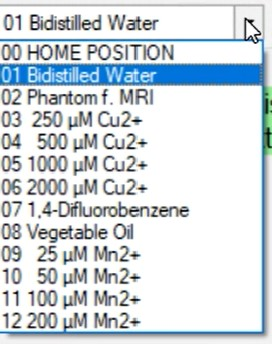
\includegraphics[width = 0.7 \textwidth]{Screenshot2/Konzentrationen_der_Messungen.jpg}
    \caption{Konzentrationen der Verfügbaren Proben}
    \end{figure}
    
\begin{figure}[H]
    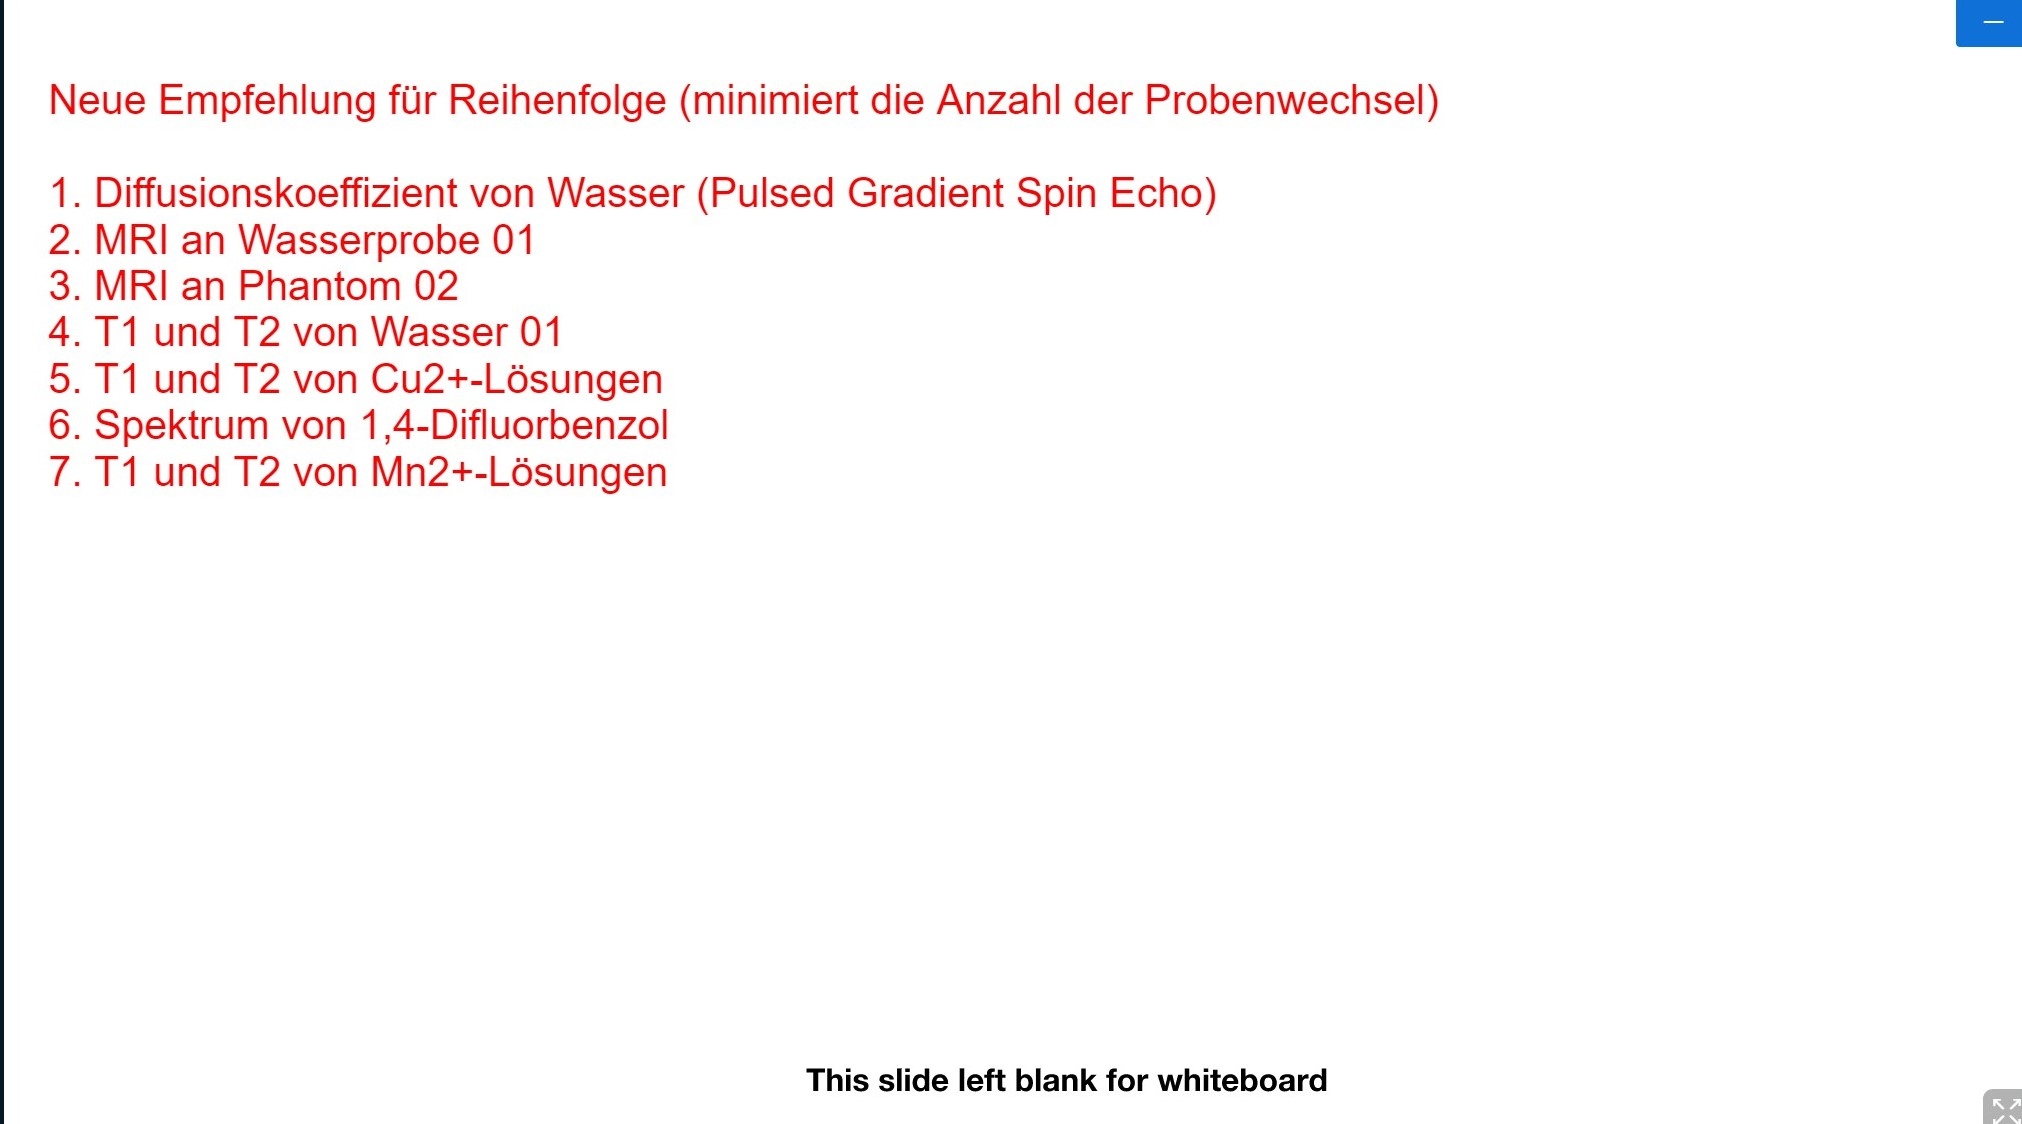
\includegraphics[width = 0.7 \textwidth]{Screenshot2/Messreihenfolge.jpg}
    \caption{neue Messreihenfolge}
\end{figure}

\begin{figure}[H]
    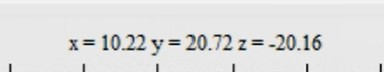
\includegraphics[width = 0.7 \textwidth]{Screenshot2/Autoshimwerte.jpg}
    \caption{Autoshimmingwerte}
\end{figure}

 \begin{tabular}{ll}   
    \textbf{Durchführung} & \\
           1.1 & Pulse and Collect (EFNMR menu): \\
           & water sample (FID und Spektrum) Polarisationszeit 4s \\
    
           1.2 & Pulse and Collect (EFNMR menu): \\
           & water sample (FID und Spektrum) kürzere polarisationszeit (500ms) \\

           1.3 & T1 Bp\\
           &  T1 dauer des wassers ermitteln in bp\\

           1.4 & T2 Messung CPMG\\
    
           2.1 & Pulse and Collect (EFNMR menu): \\
           & doped water sample 1 (FID und Spektrum) Polaraisationszeit 4s \\
    
           2.2 & Pulse and Collect (EFNMR menu): \\
           &doped water sample 1 (FID und Spektrum) kürzere polarisationszeit (500ms) \\

           2.3 & Pulse and Collect (EFNMR menu): \\
           & doped water sample 2 (FID und Spektrum) Polaraisationszeit 4s \\
    
           2.4 & Pulse and Collect (EFNMR menu): \\
           & doped water sample 2 (FID und Spektrum) kürzere polarisationszeit (500ms) \\ 

           3.1 & doped water sample 1 Cu2+: T2 Messung: 250 $\mu$ M in 500ml Wasser \\
    
           3.2 & doped water sample 1: T1 Messung (Polarisationsfeld): 250 $\mu$ M in 500ml Wasser \\
    
           4.1 & doped water sample 1: T2 Messung: 500 $\mu$ M in 500ml Wasser \\
    
           4.2 & doped water sample 1: T1 Messung (Polarisationsfeld): 500 $\mu$ M in 500ml Wasser \\

           5.1 & doped water sample 1: T2 Messung: 1000 $\mu$ M in 500ml Wasser \\
    
           5.2 & doped water sample 1: T1 Messung (Polarisationsfeld): 1000 $\mu$ M in 500ml Wasser \\

           6.1 & doped water sample 1: T2 Messung: 2000 $\mu$ M in 500ml Wasser \\
    
           6.2 & doped water sample 1: T1 Messung (Polarisationsfeld): 2000 $\mu$ M in 500ml Wasser \\

        %    7.1 & doped water sample 1: T2 Messung: 4000 $\mu$ M in 500ml Wasser \\
    
        %    7.2 & doped water sample 1: T1 Messung (Polarisationsfeld): 4000 $\mu$ M in 500ml Wasser \\

           7.3 & doped water sample 2 Mangan Ma2+: T2 Messung: 25 $\mu$ M in 500ml Wasser \\
    
           7.4 & doped water sample 2: T1 Messung (Polarisationsfeld): 25 $\mu$ M in 500ml Wasser \\
    
           7.5 & doped water sample 2: T2 Messung: 50 $\mu$ M in 500ml Wasser \\
    
           7.6 & doped water sample 2: T1 Messung (Polarisationsfeld): 50 $\mu$ M in 500ml Wasser \\

           7.7 & doped water sample 2: T2 Messung: 100 $\mu$ M in 500ml Wasser \\
    
           7.8 & doped water sample 2: T1 Messung (Polarisationsfeld): 100 $\mu$ M in 500ml Wasser \\

           7.9 & doped water sample 2: T2 Messung: 200 $\mu$ M in 500ml Wasser \textcolor{red}{7.9 niedriger duellecho ist richtige Datei!!!} \\
    
           7.10 & doped water sample 2: T1 Messung (Polarisationsfeld): 200 $\mu$ M in 500ml Wasser \\

        %    7.11 & doped water sample 2: T2 Messung: 4000 $\mu$ M in 500ml Wasser \\
    
        %    7.12 & doped water sample 2: T1 Messung (Polarisationsfeld): 4000 $\mu$ M in 500ml Wasser \\
    \end{tabular}  
     
    \begin{figure}[H]
        \centering
        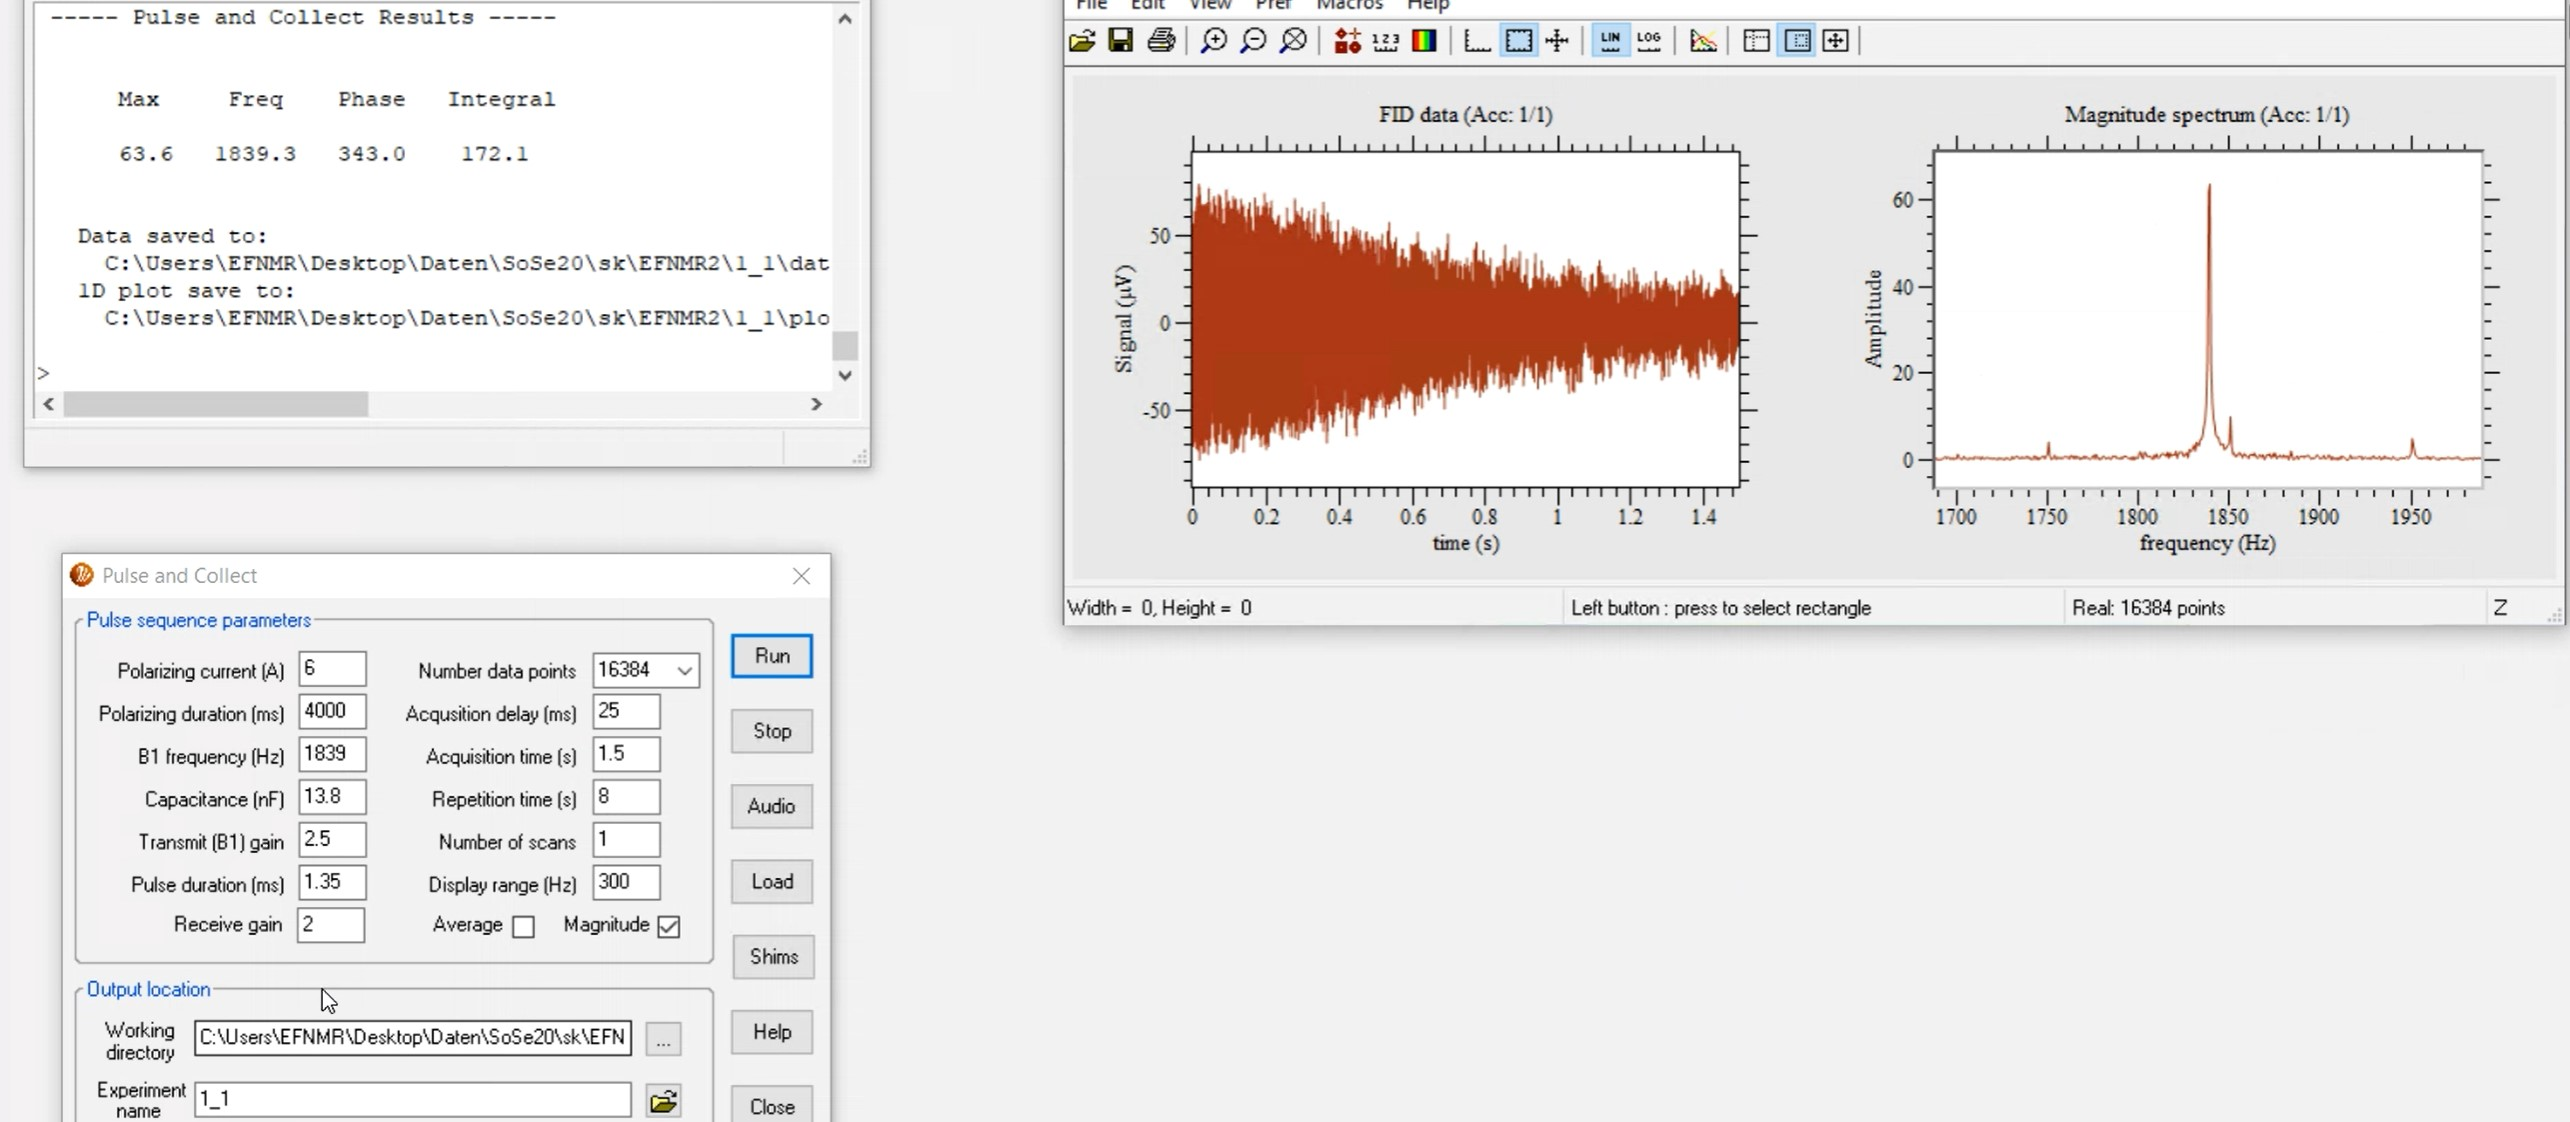
\includegraphics[width = 0.8\textwidth]{Screenshot2/1_1.jpg}
        \caption{1.1}
    \end{figure}
    \begin{figure}[H]
        \centering
        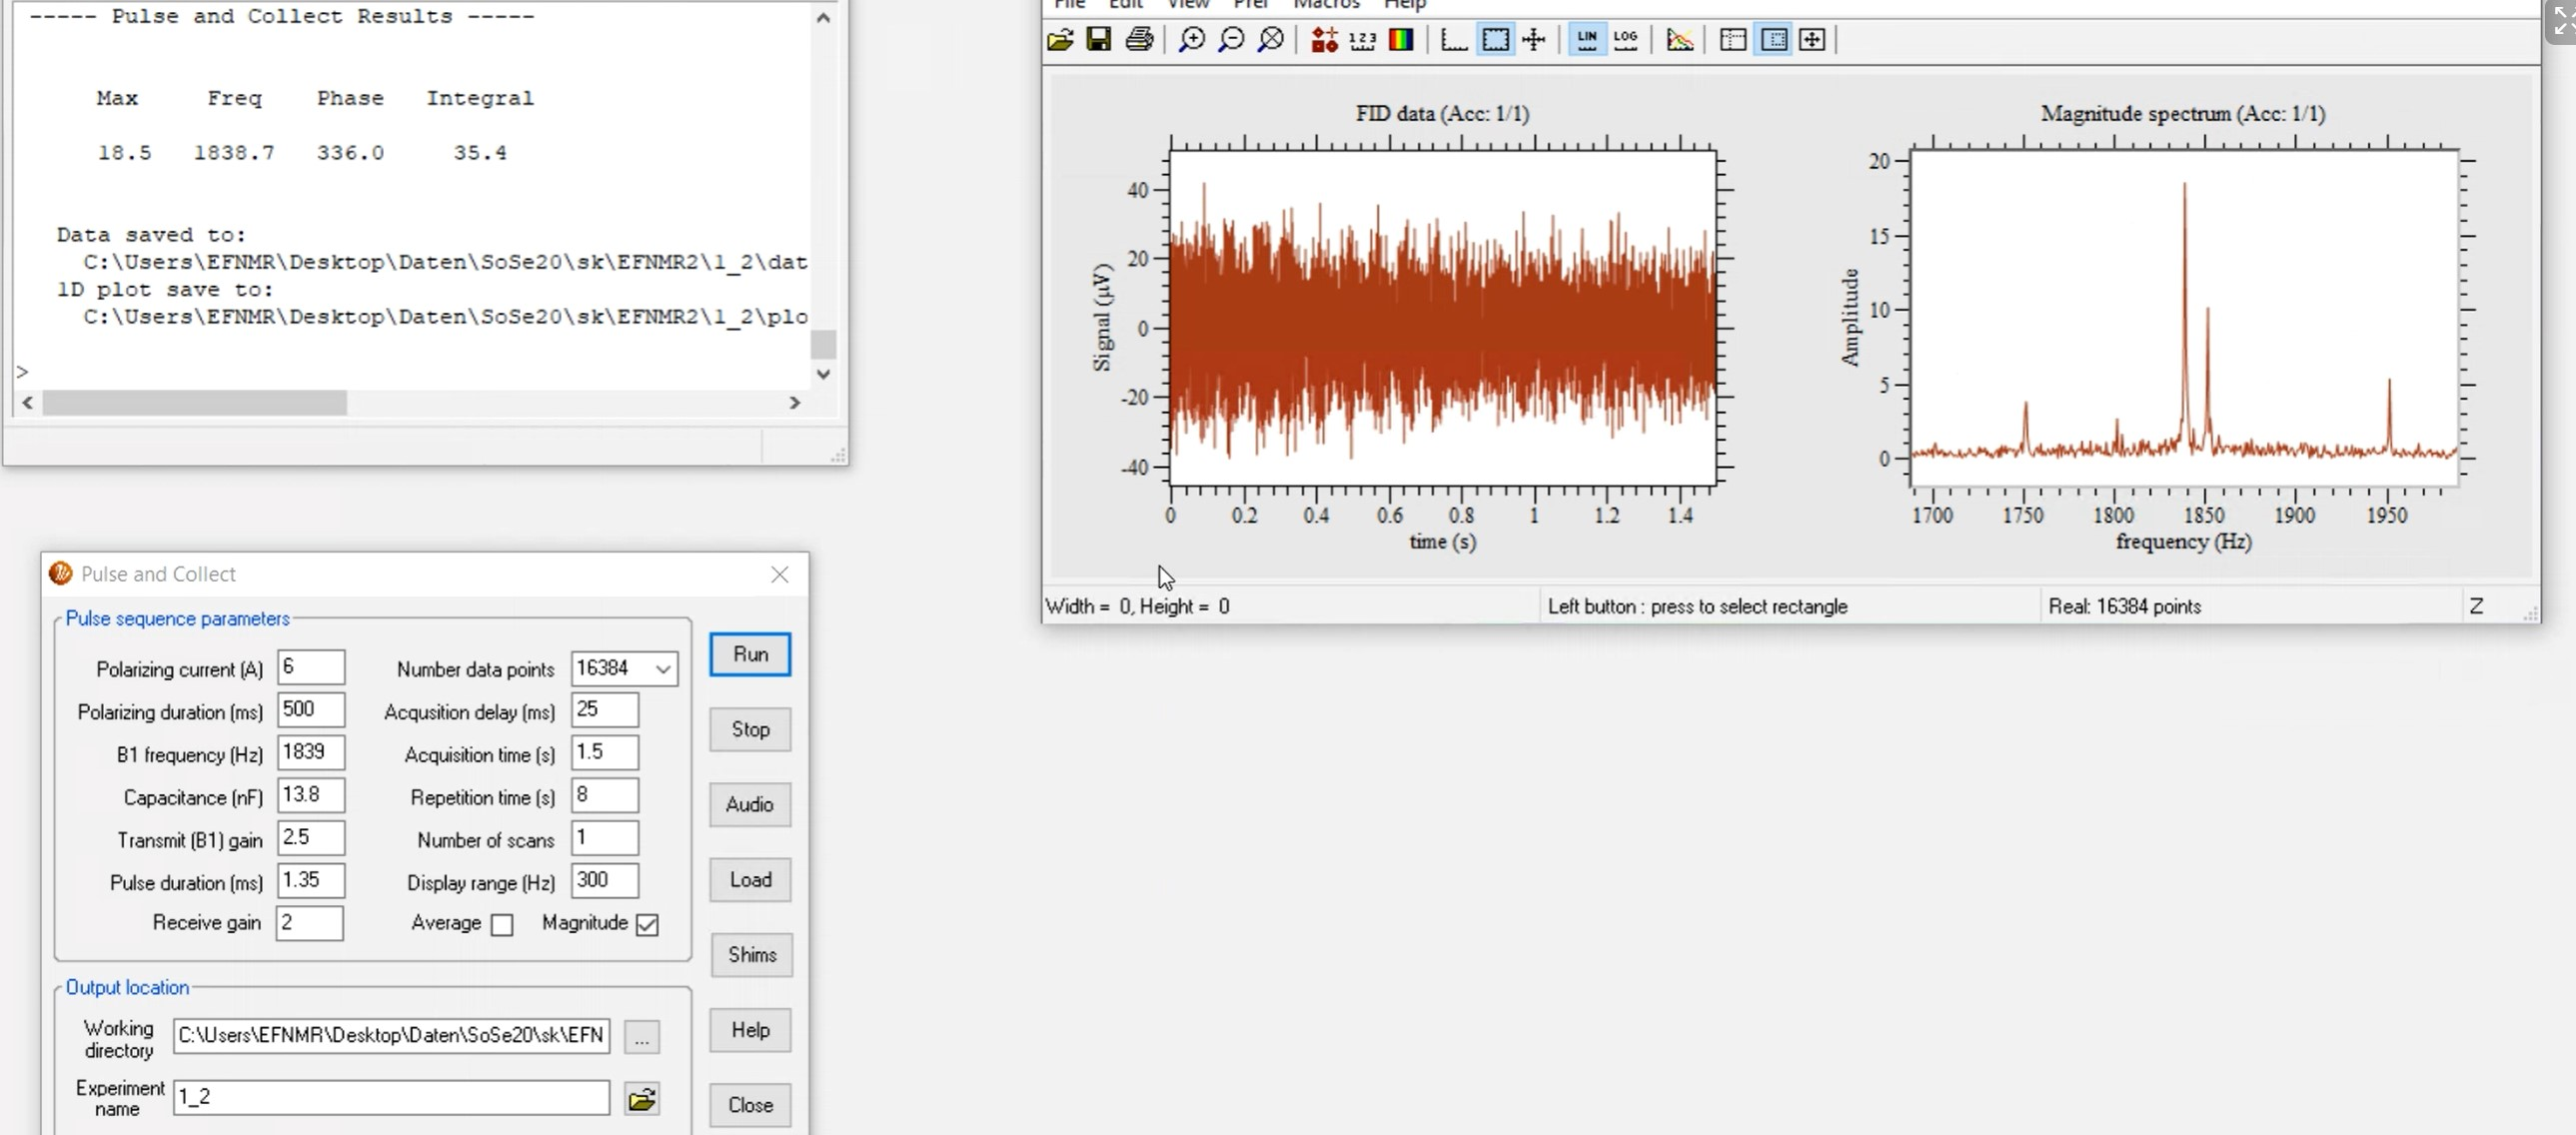
\includegraphics[width = 0.8\textwidth]{Screenshot2/1_2.jpg}
        \caption{1.2}
    \end{figure}
    \begin{figure}[H]
        \centering
        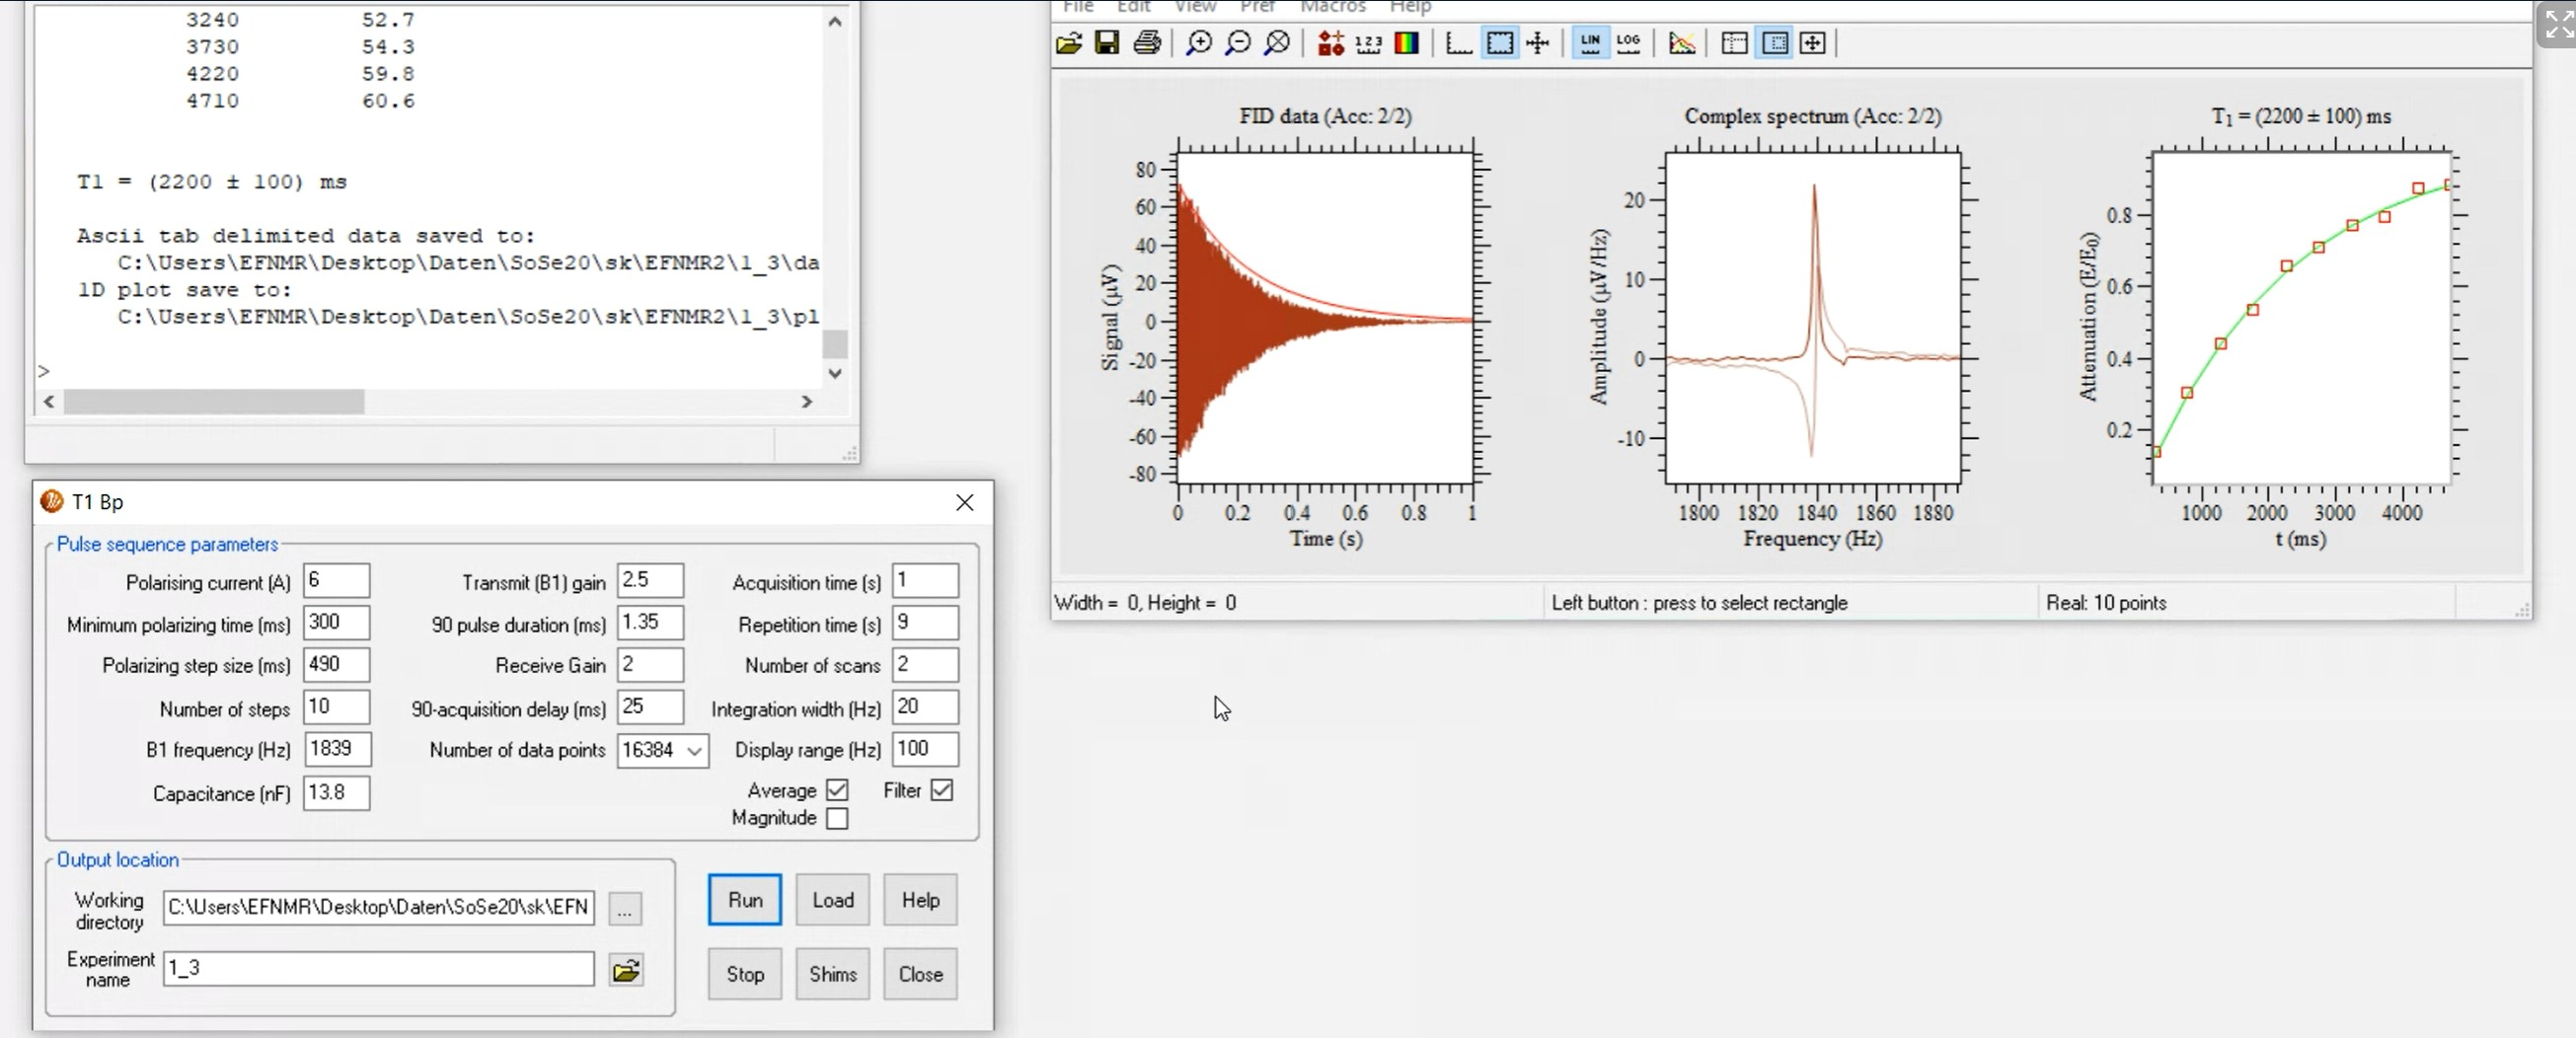
\includegraphics[width = 0.8\textwidth]{Screenshot2/1_3.jpg}
        \caption{1.3}
    \end{figure}
    \begin{figure}[H]
        \centering
        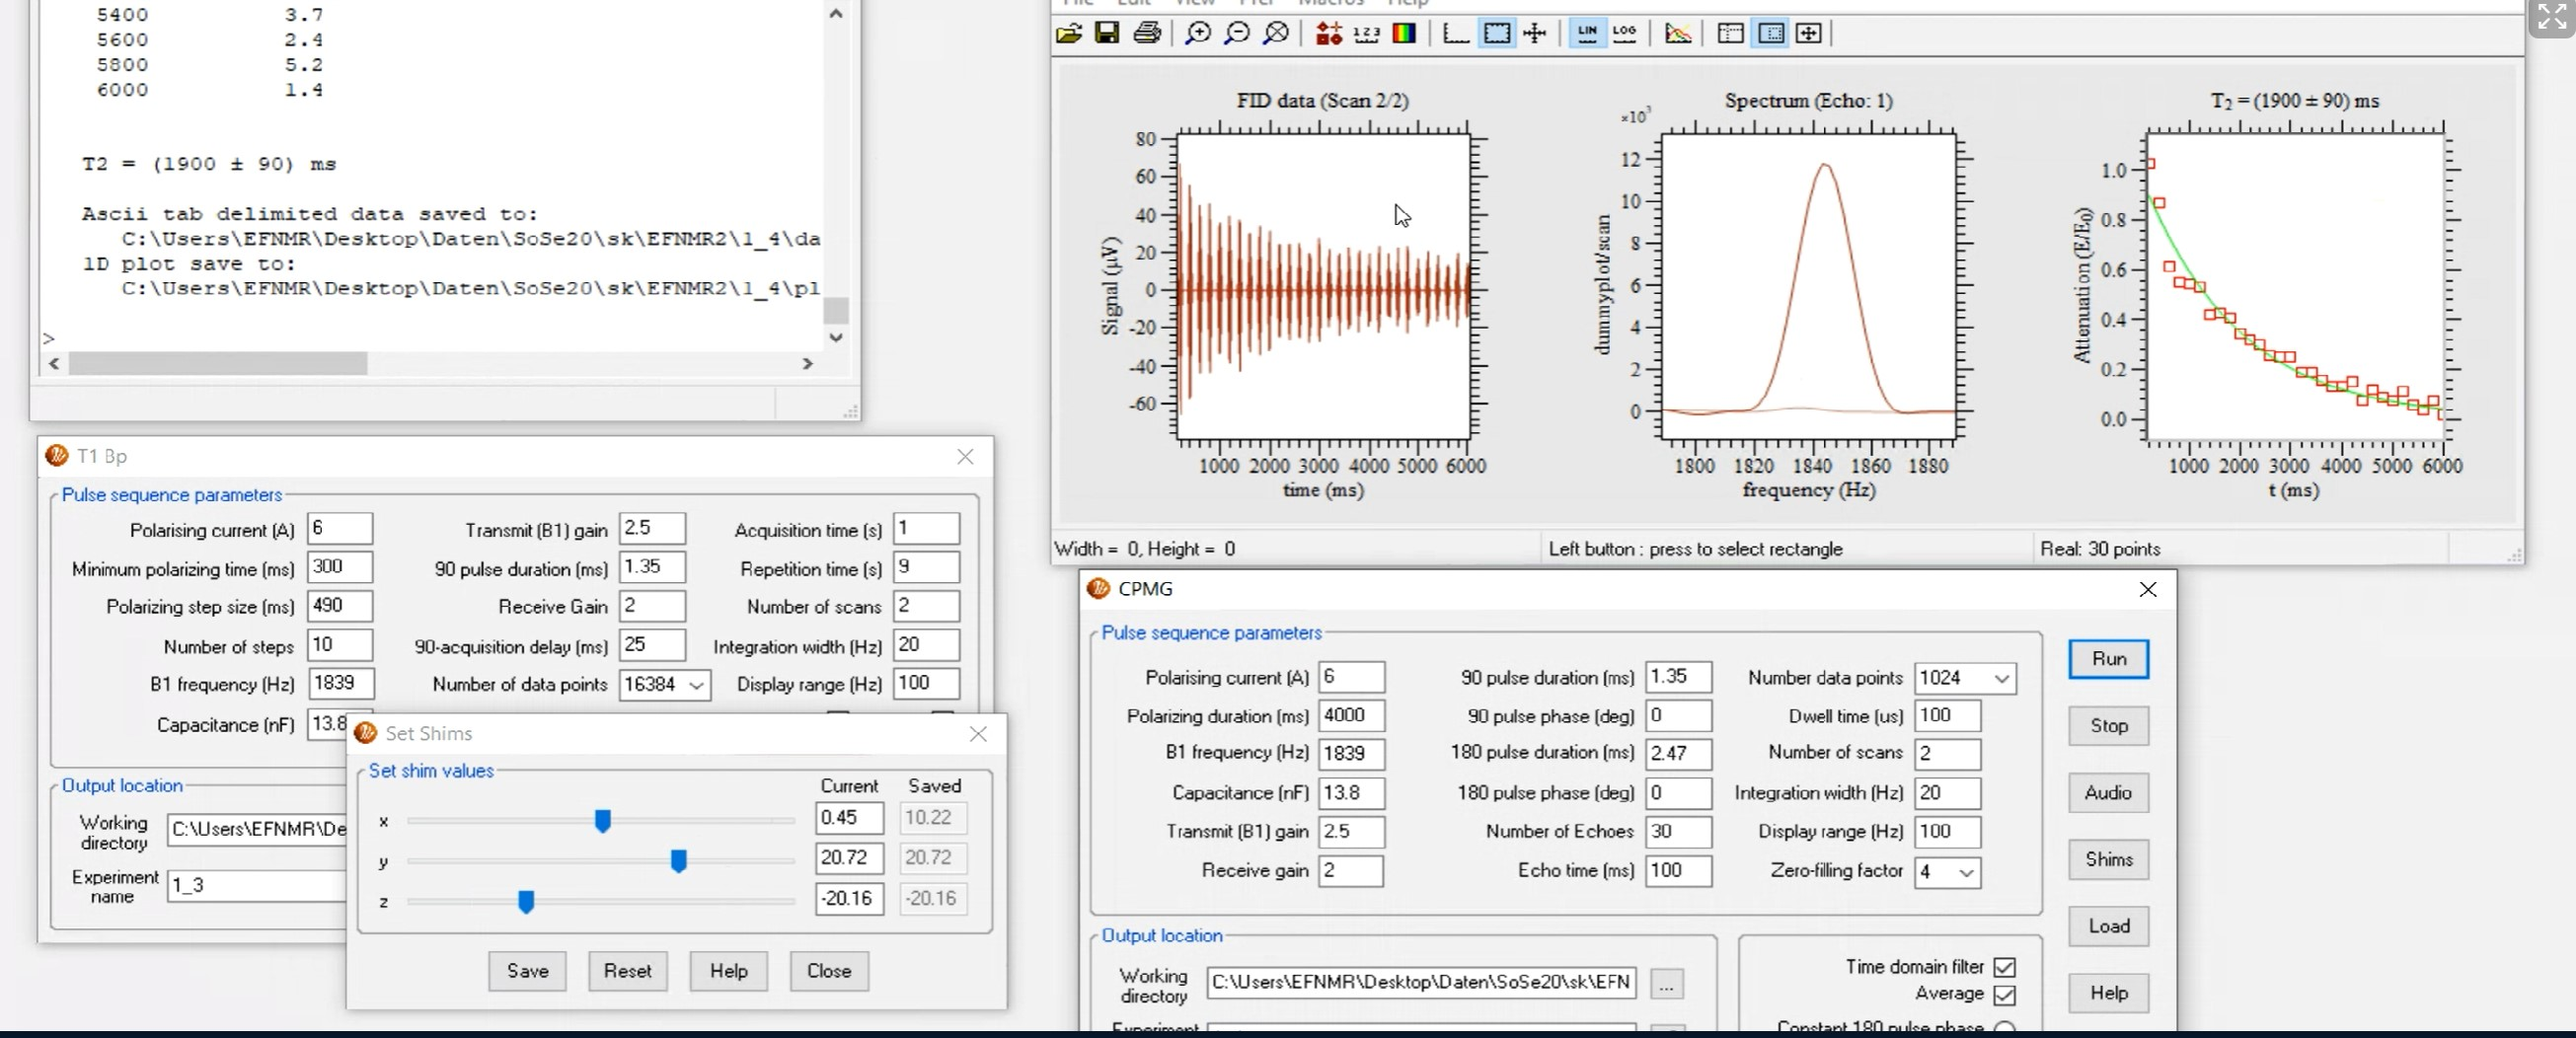
\includegraphics[width = 0.8\textwidth]{Screenshot2/1_4.jpg}
        \caption{1.4}
    \end{figure}
    \begin{figure}[H]
        \centering
        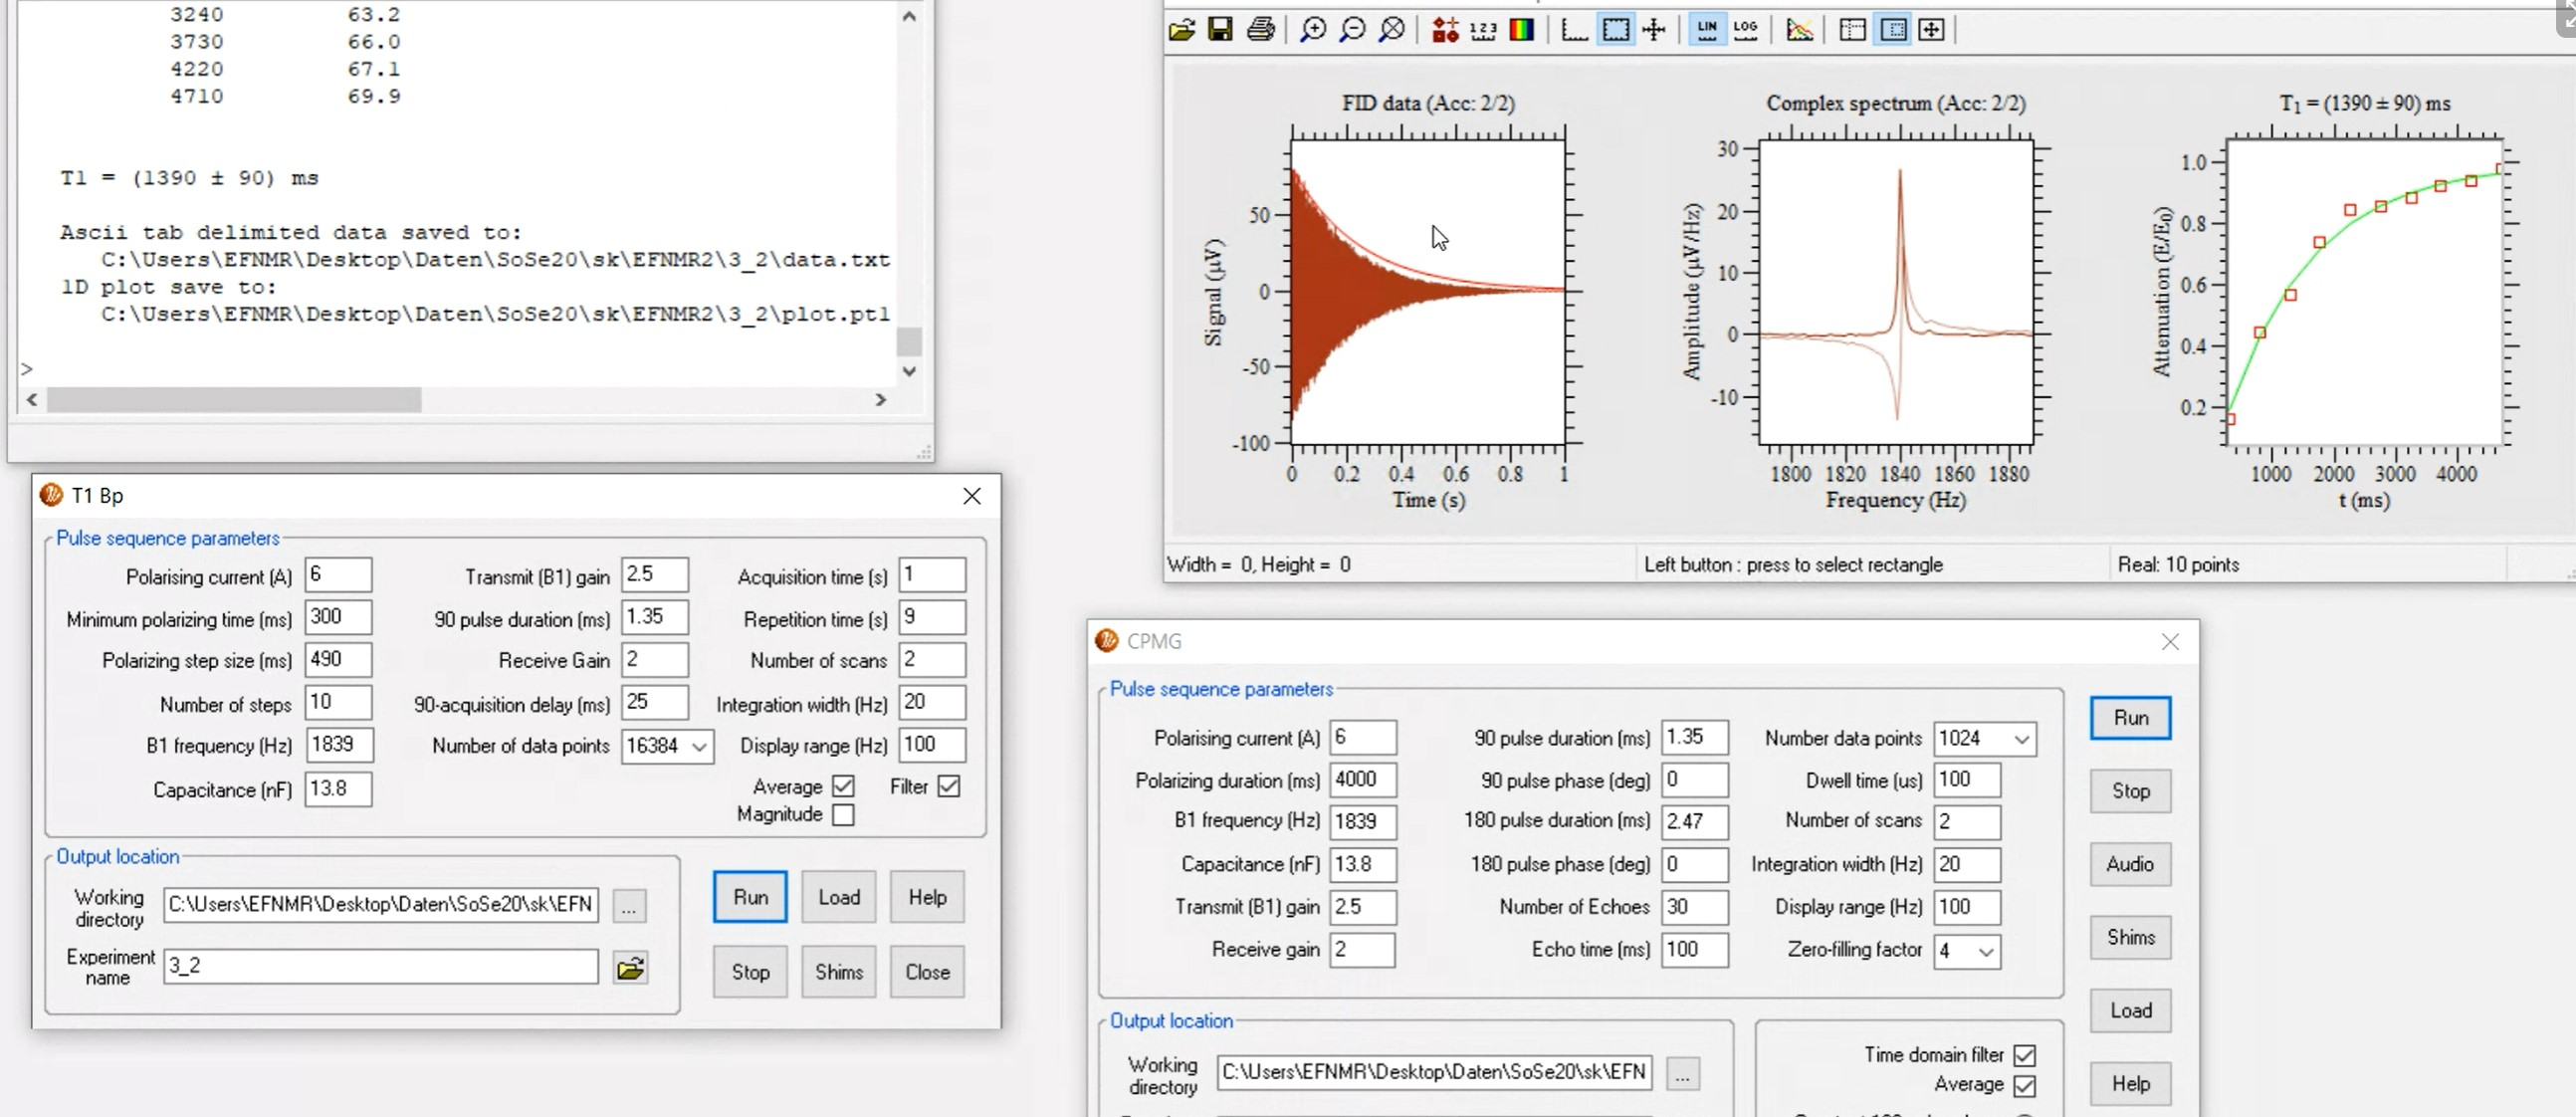
\includegraphics[width = 0.8\textwidth]{Screenshot2/3_2.jpg}
        \caption{3.2}
    \end{figure}
    \begin{figure}[H]
        \centering
        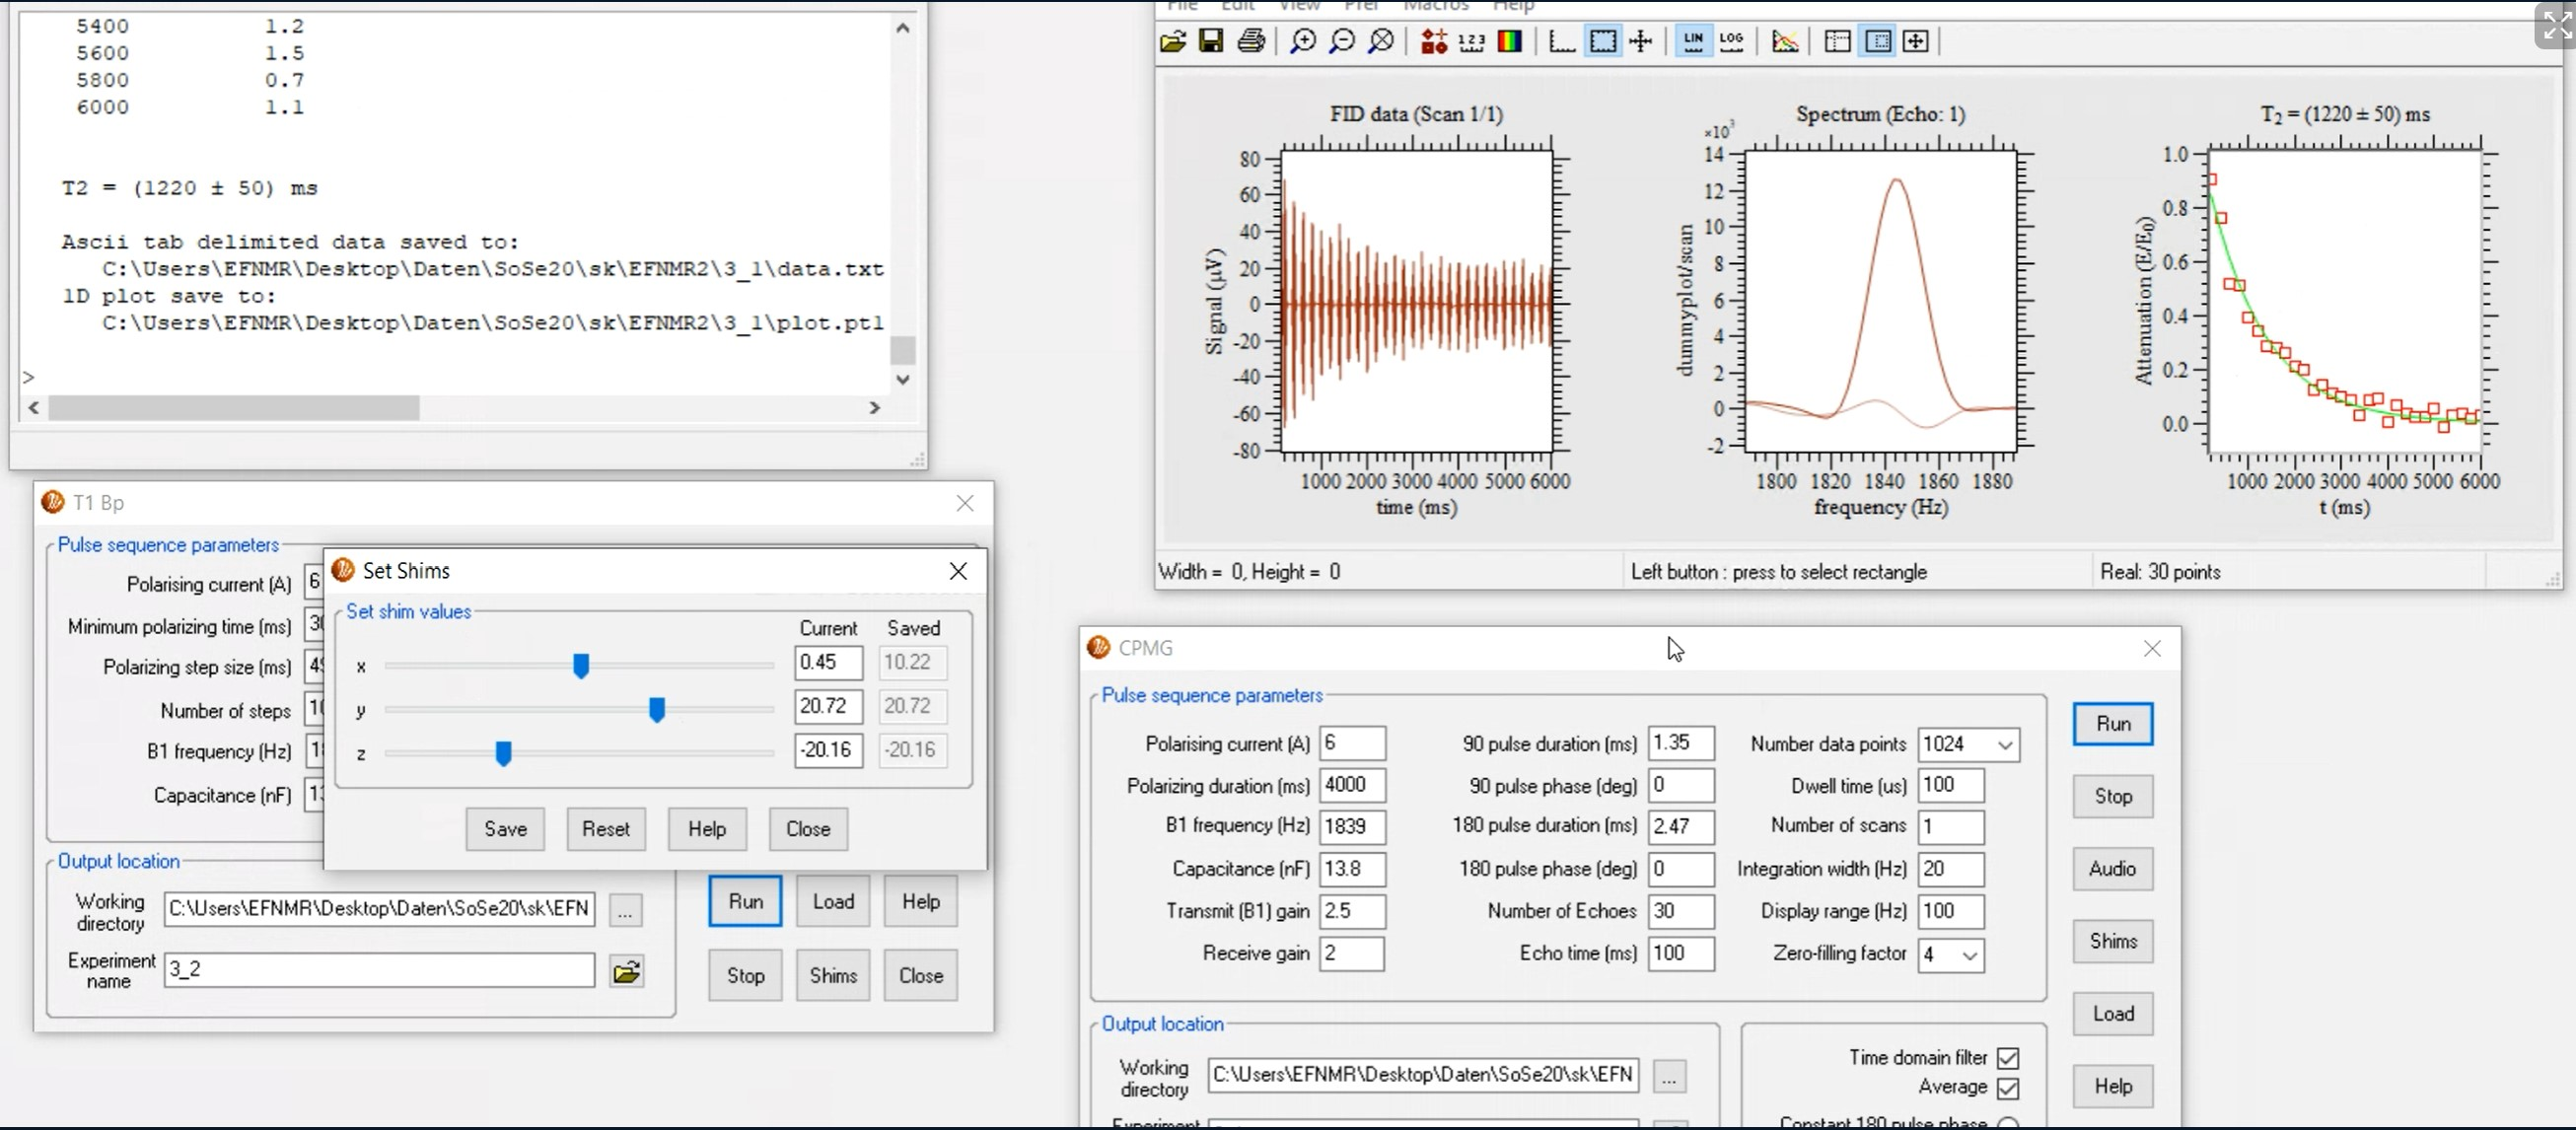
\includegraphics[width = 0.8\textwidth]{Screenshot2/3_1.jpg}
        \caption{3.1}
    \end{figure}
    \begin{figure}[H]
        \centering
        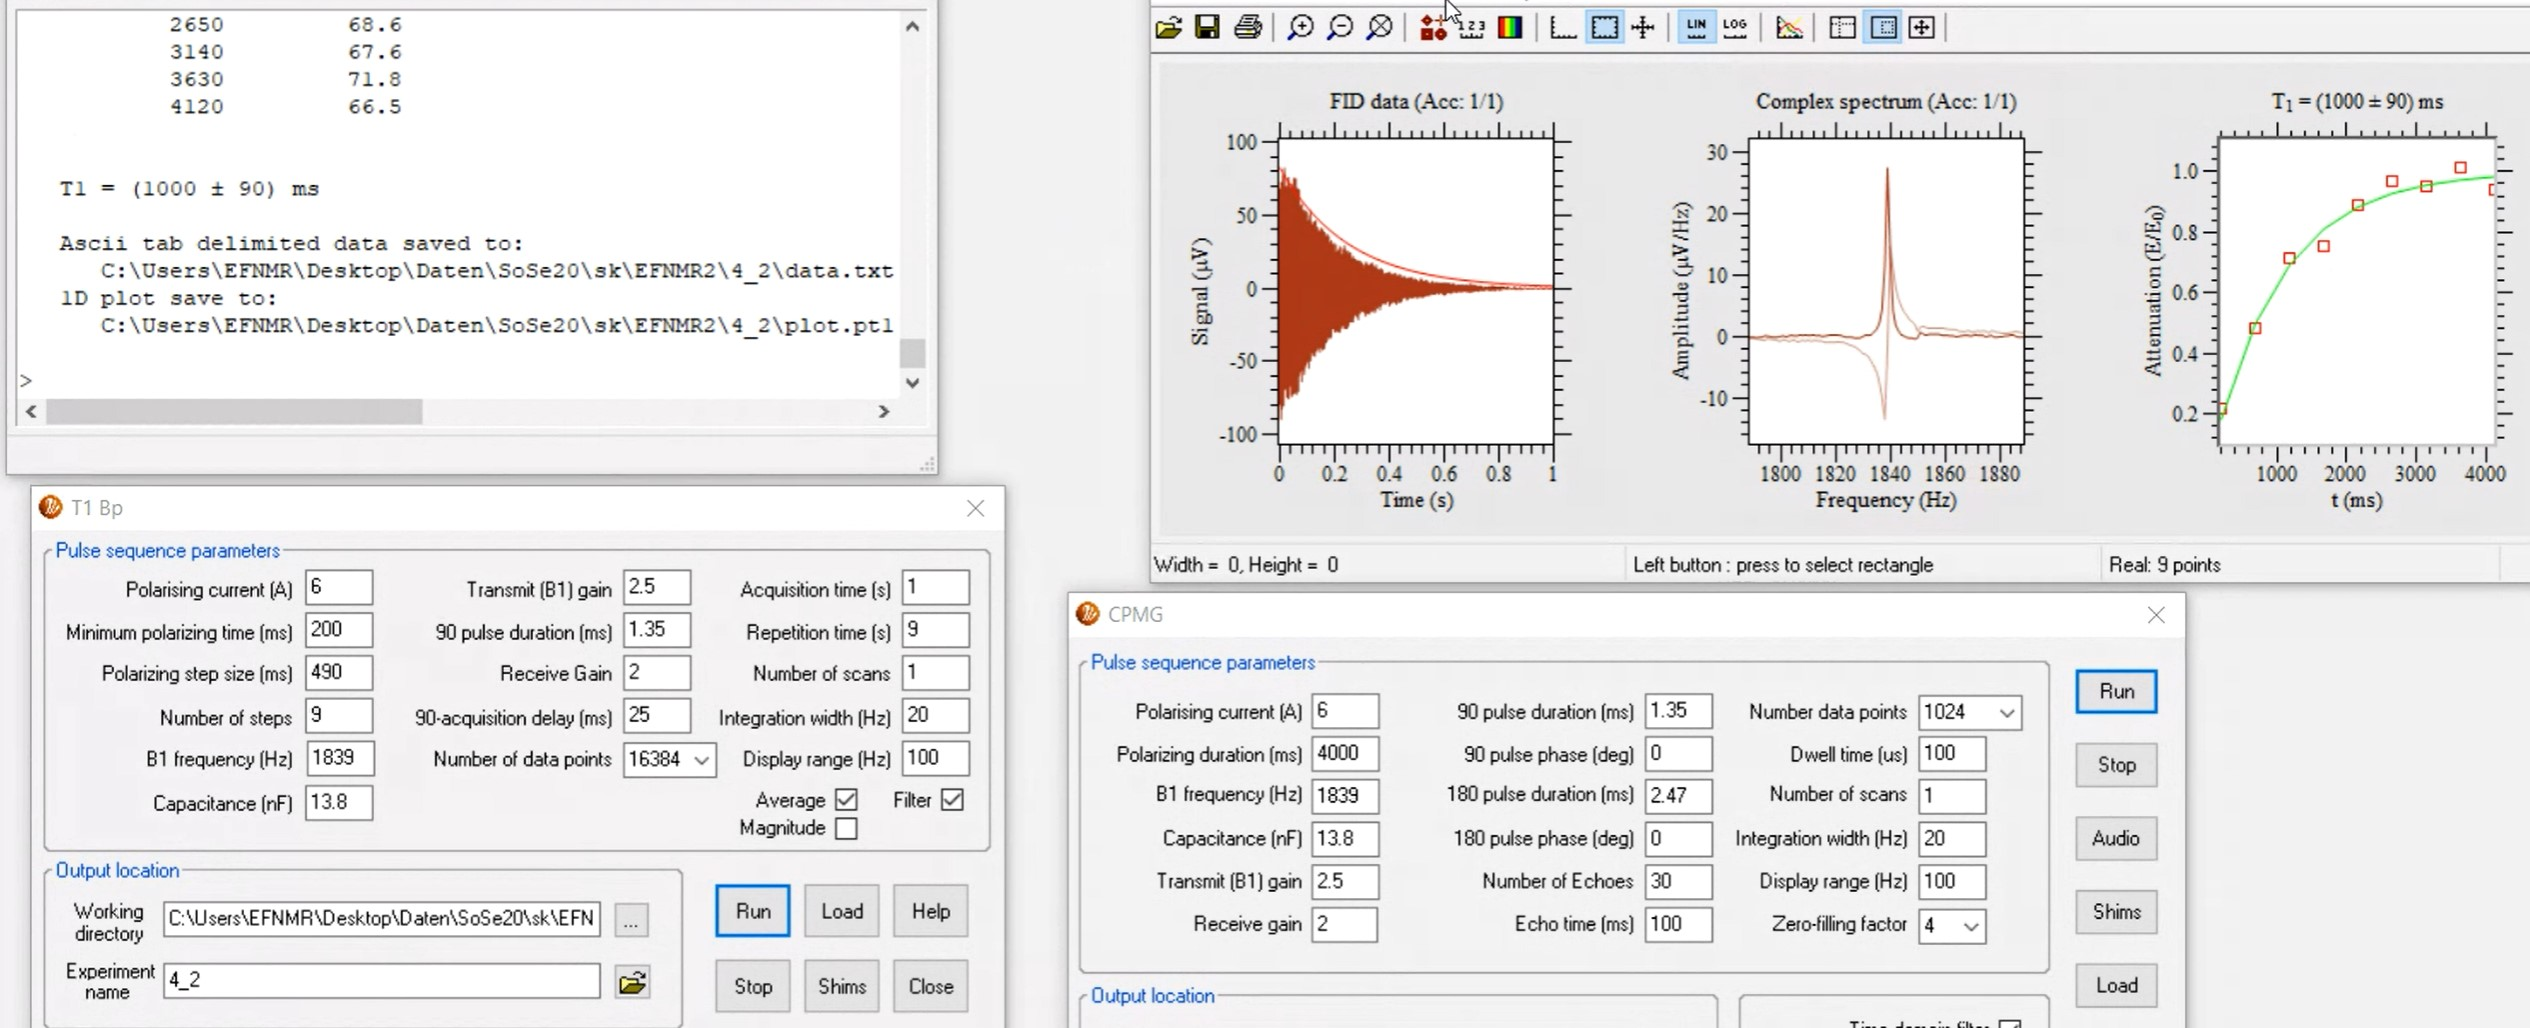
\includegraphics[width = 0.8\textwidth]{Screenshot2/4_2.jpg}
        \caption{4.2}
    \end{figure}
    \begin{figure}[H]
        \centering
        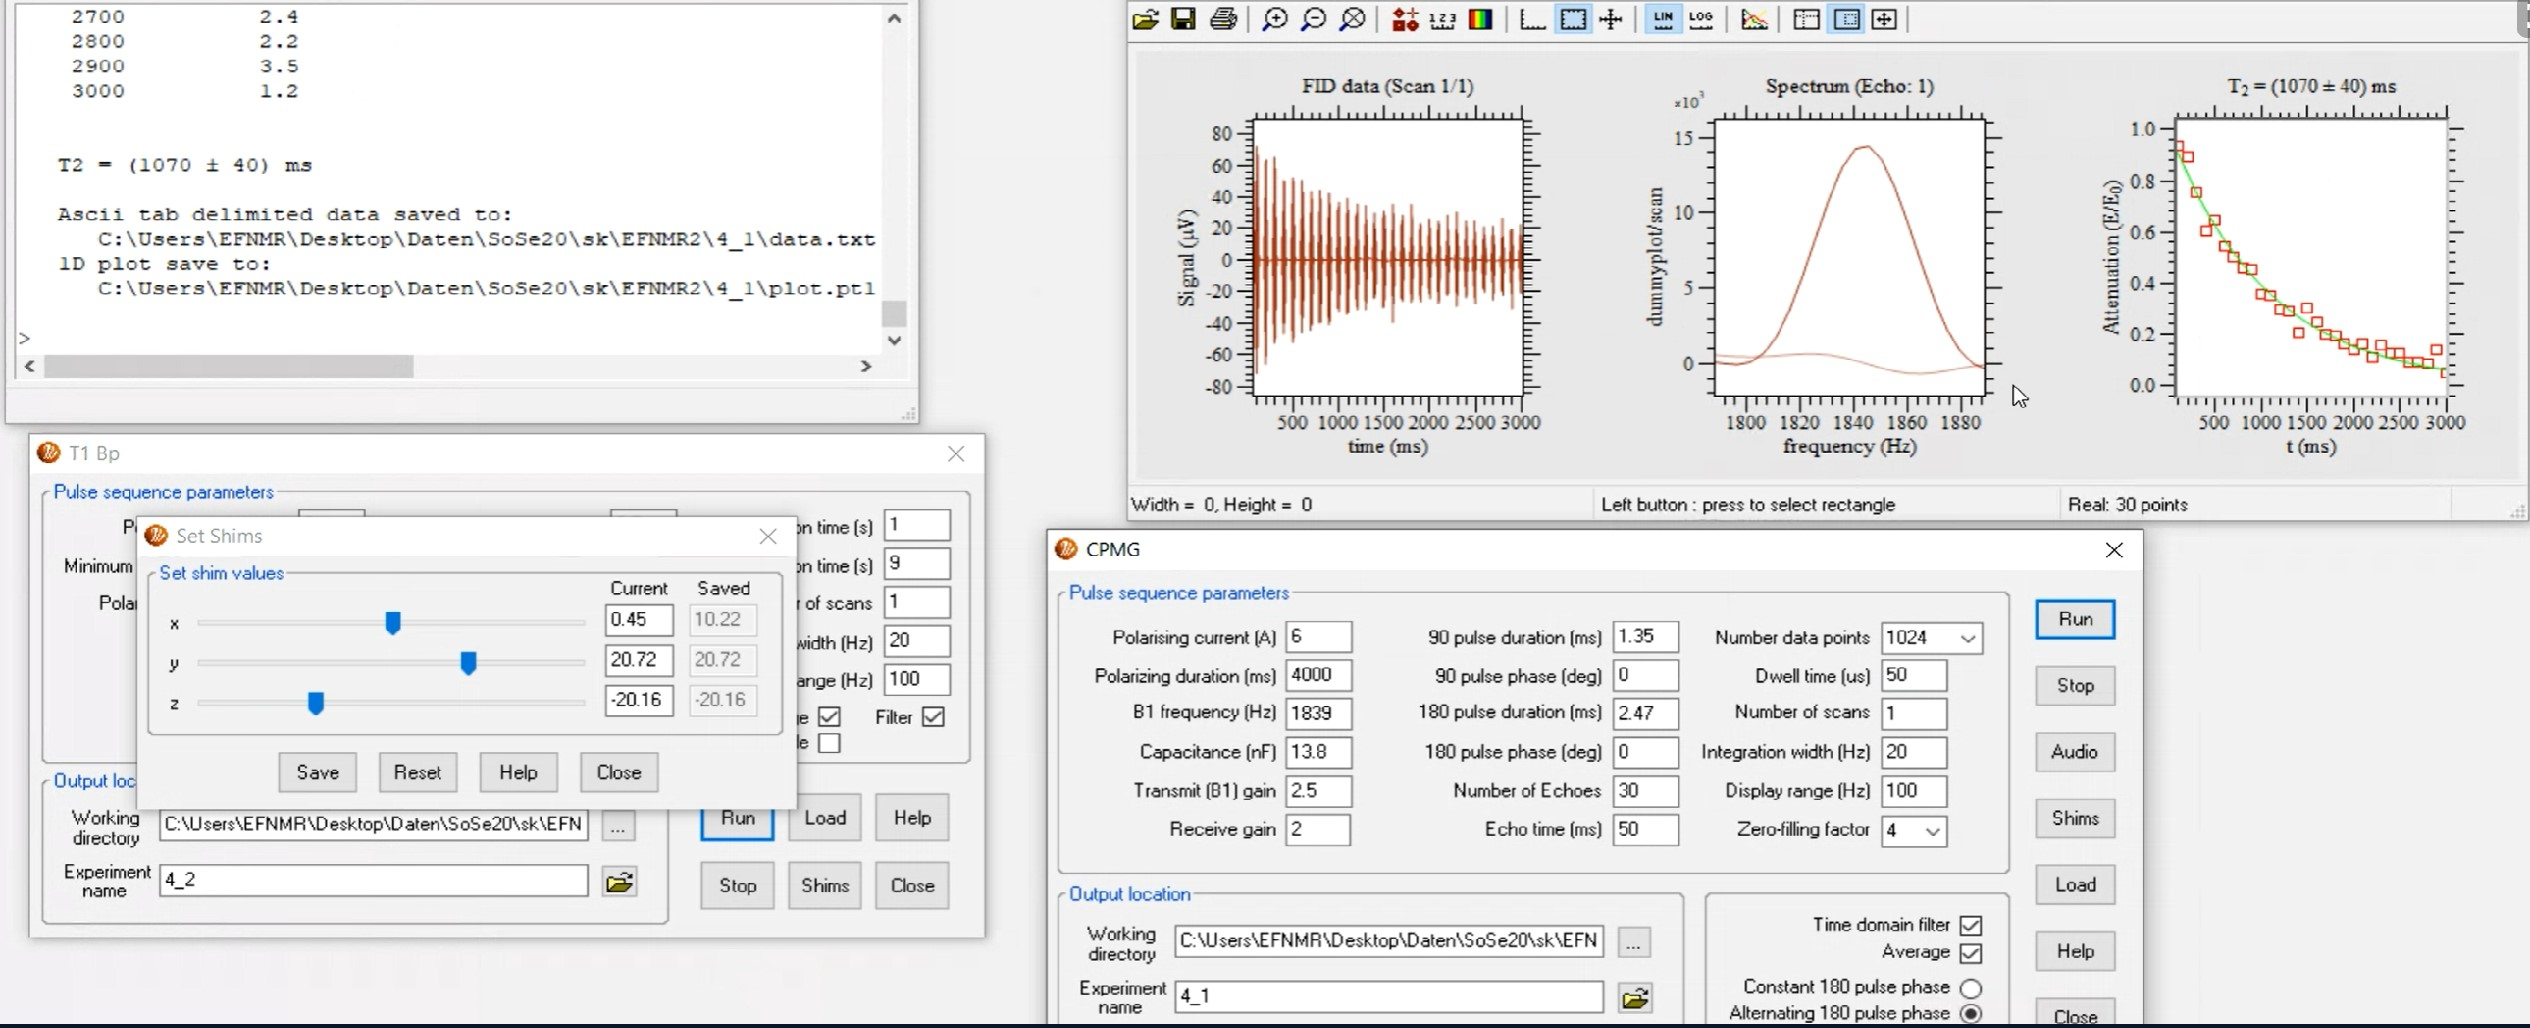
\includegraphics[width = 0.8\textwidth]{Screenshot2/4_1.jpg}
        \caption{4.1}
    \end{figure}
    \begin{figure}[H]
        \centering
        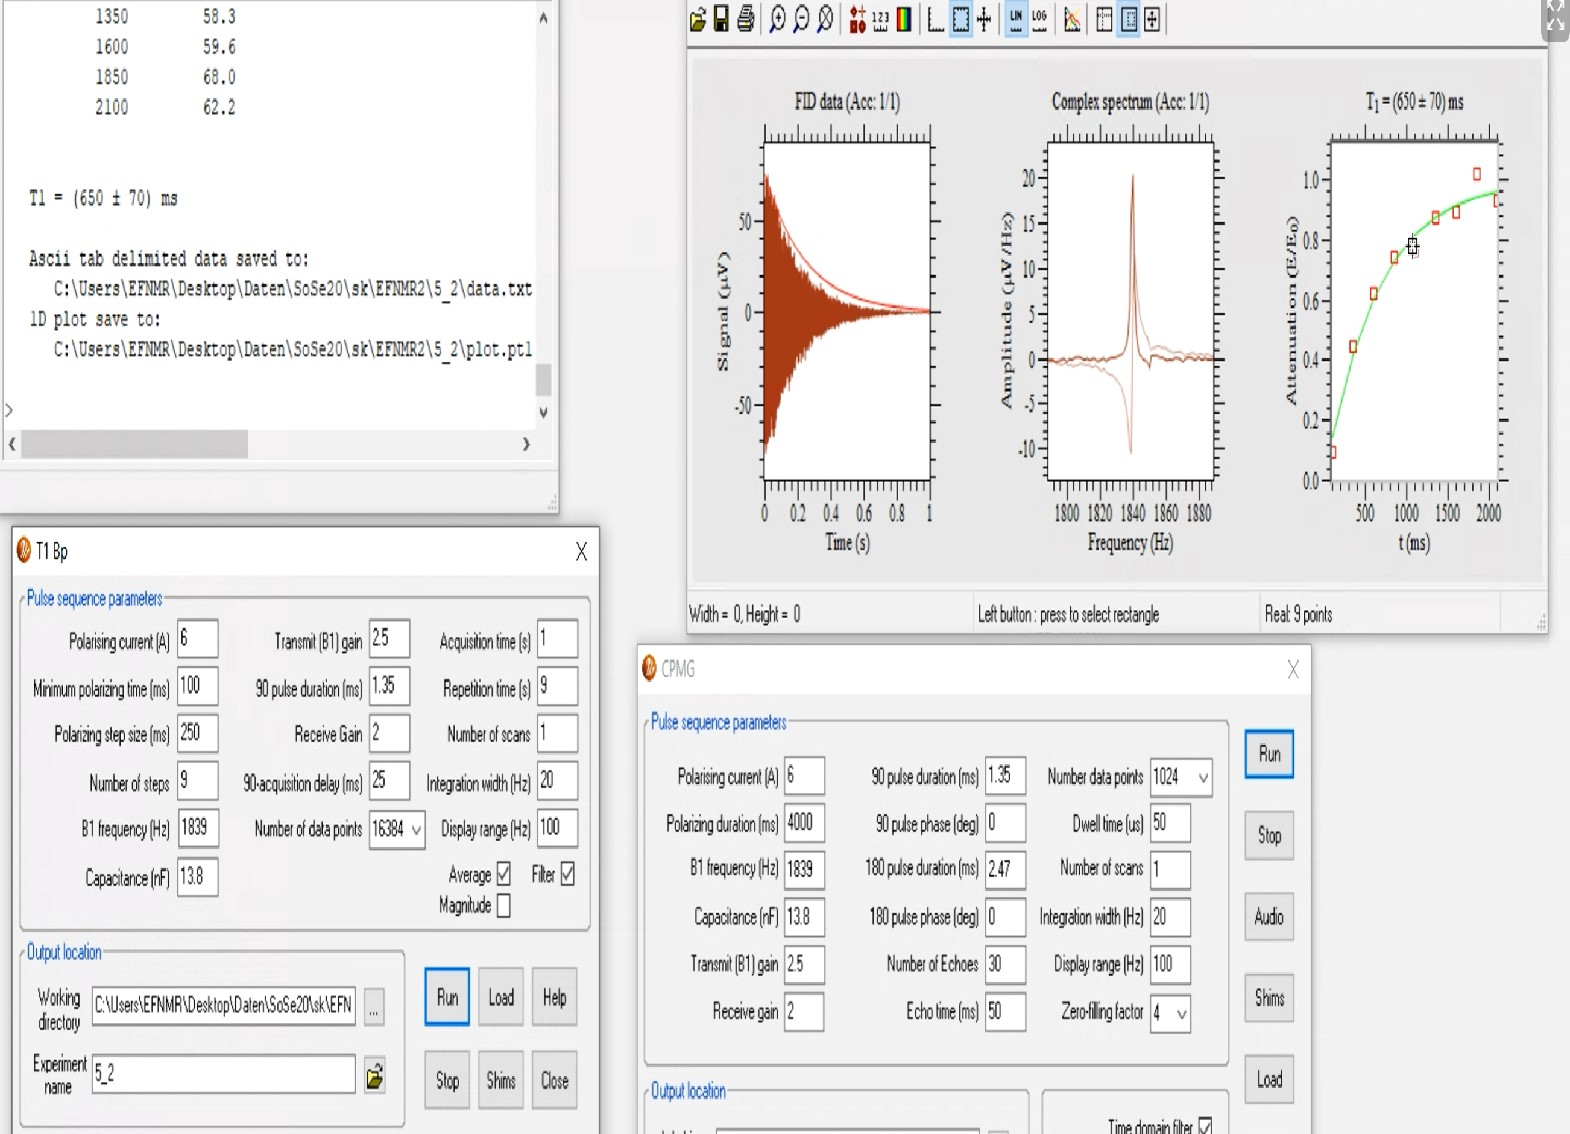
\includegraphics[width = 0.8\textwidth]{Screenshot2/5_2.jpg}
        \caption{5.2}
    \end{figure}
    \begin{figure}[H]
        \centering
        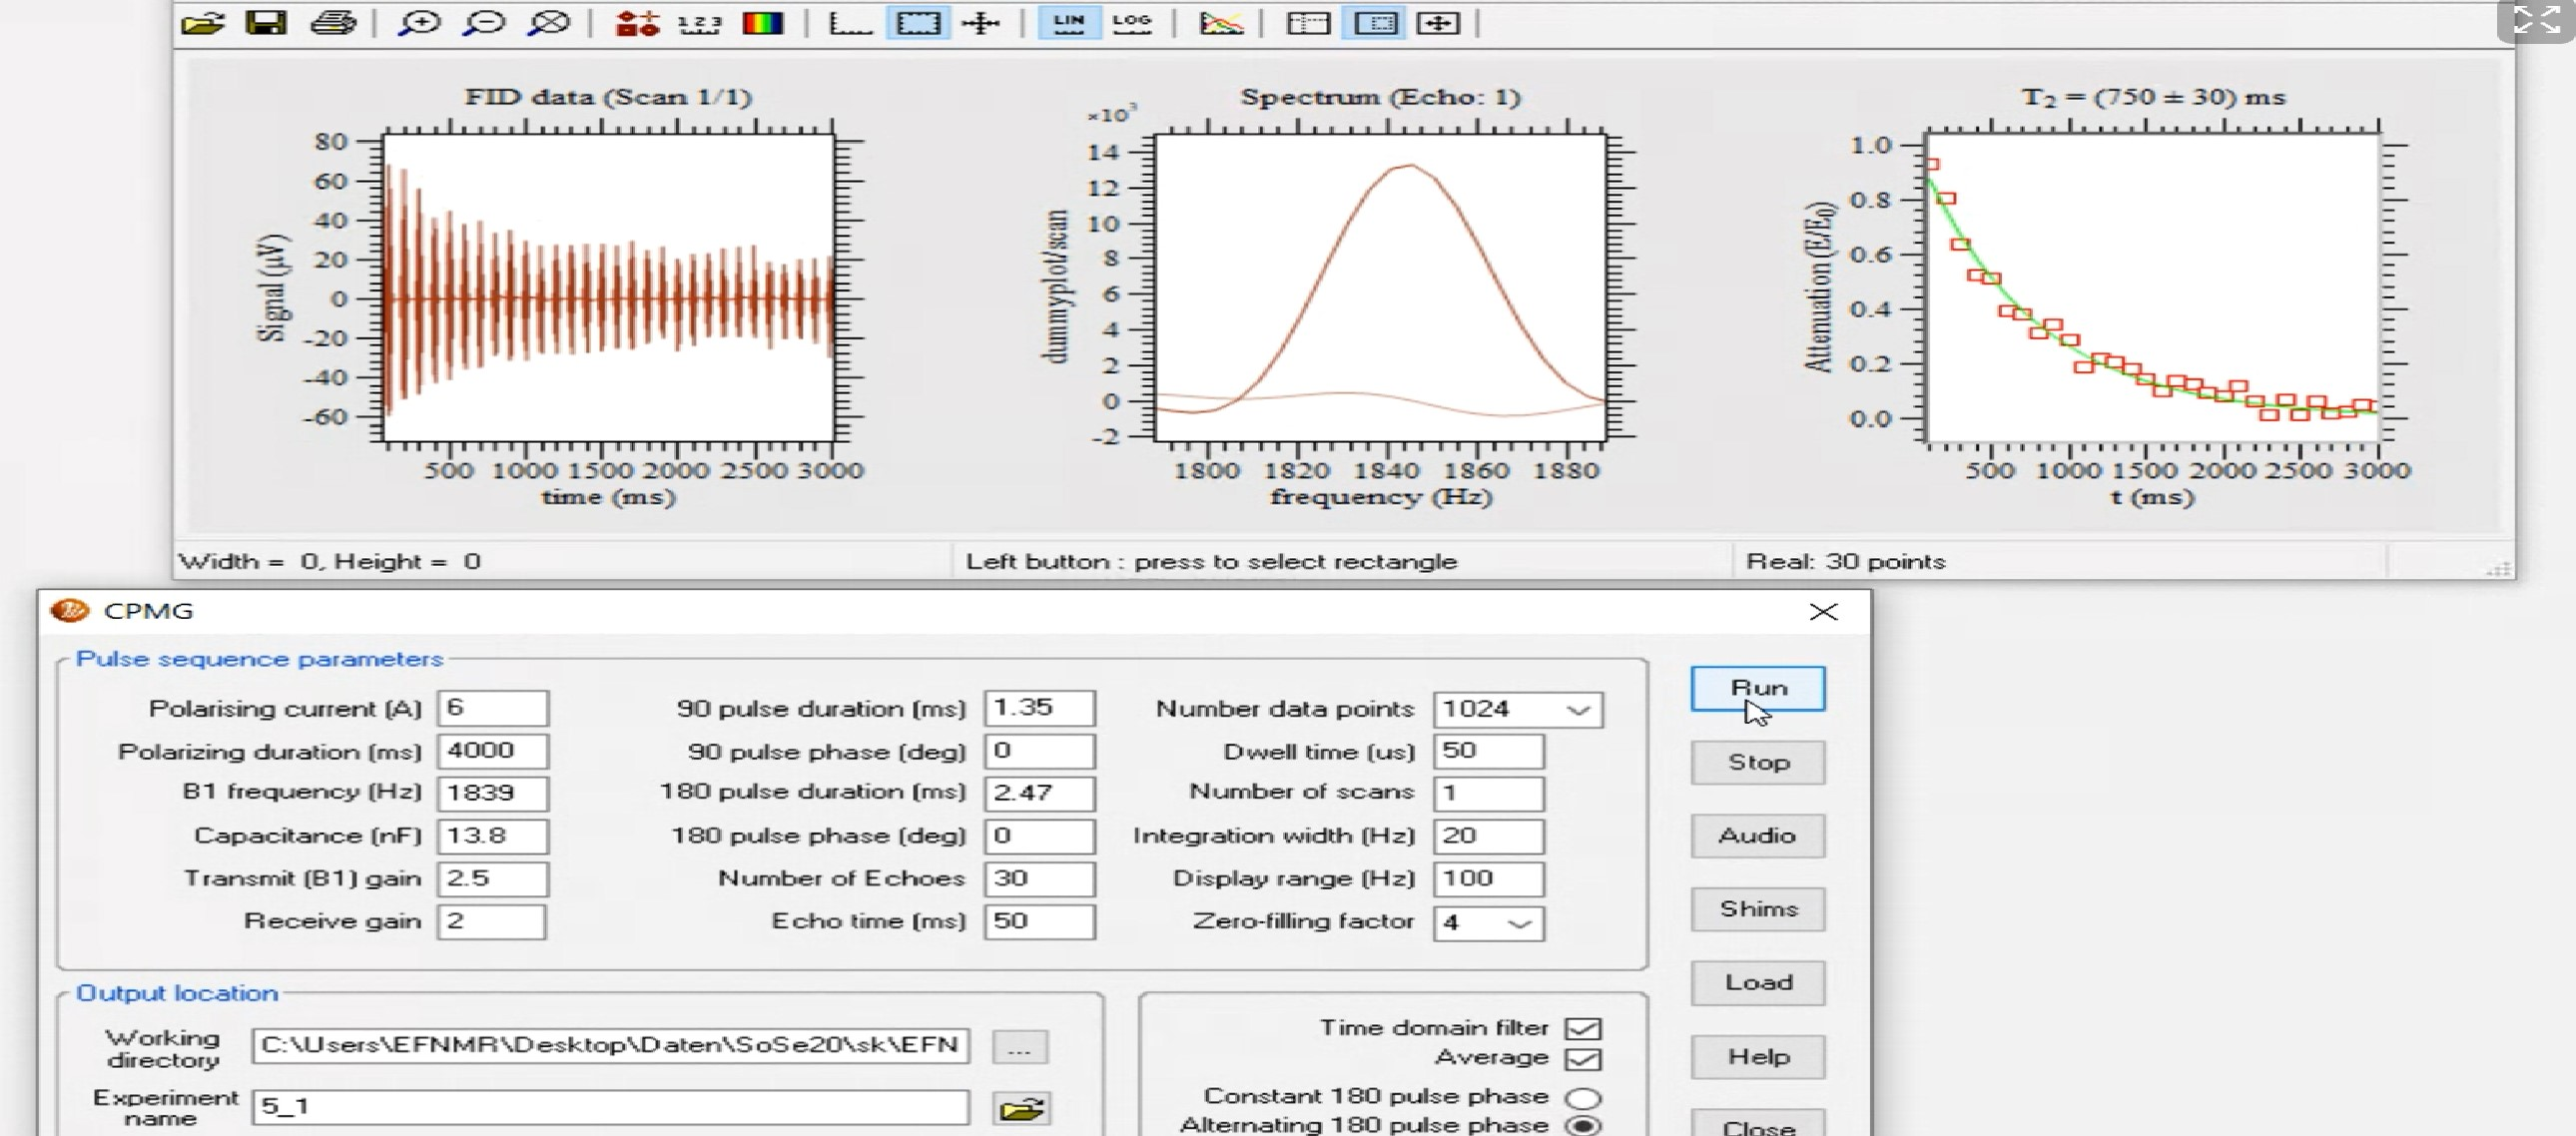
\includegraphics[width = 0.8\textwidth]{Screenshot2/5_1.jpg}
        \caption{5.1}
    \end{figure}
    \begin{figure}[H]
        \centering
        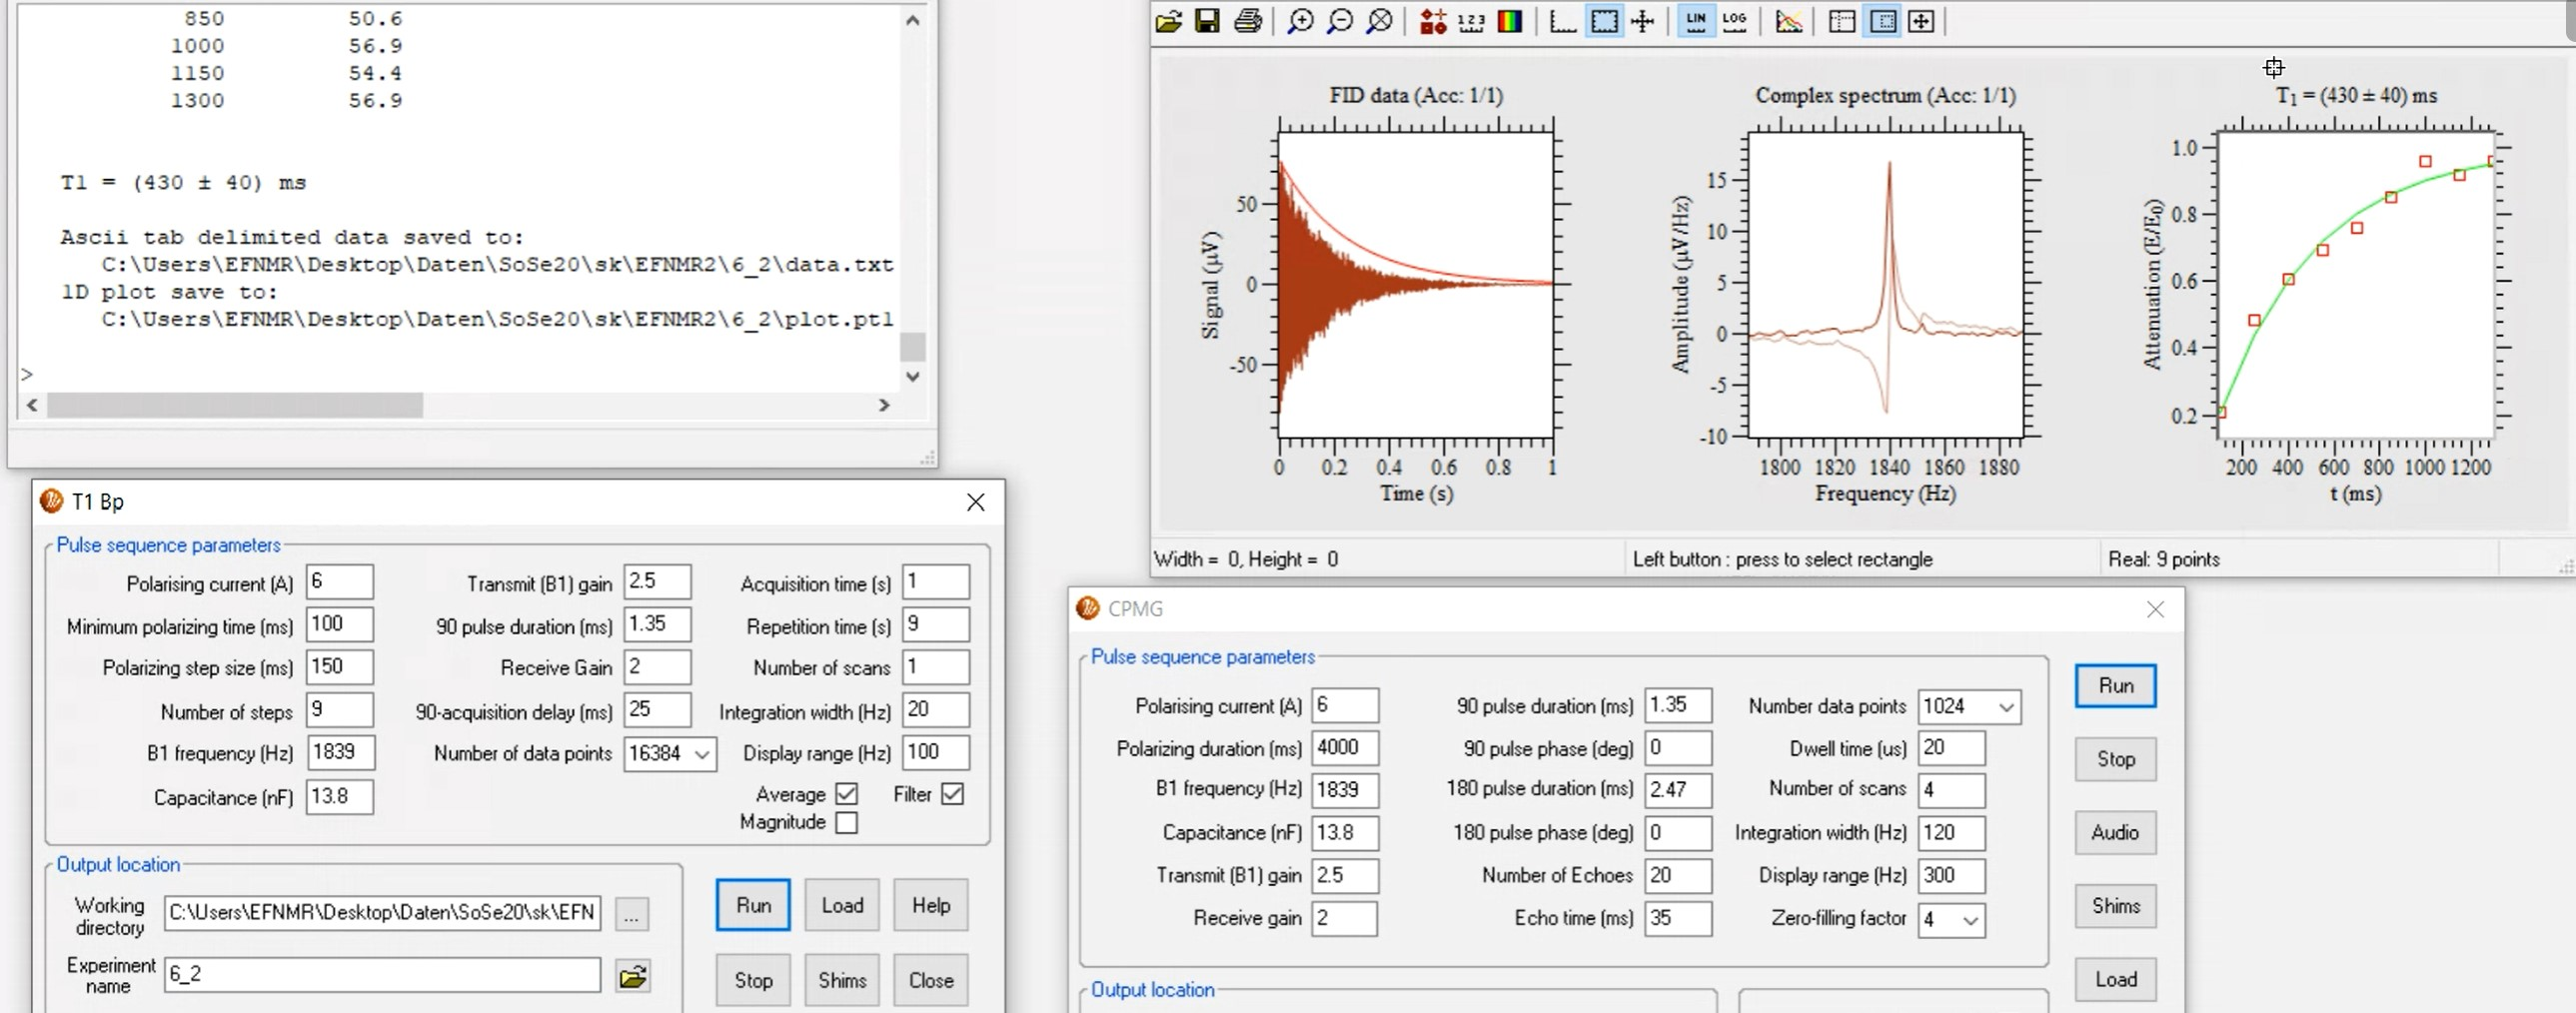
\includegraphics[width = 0.8\textwidth]{Screenshot2/6_2.jpg}
        \caption{6.2}
    \end{figure}

    \begin{figure}[H]
        \centering
        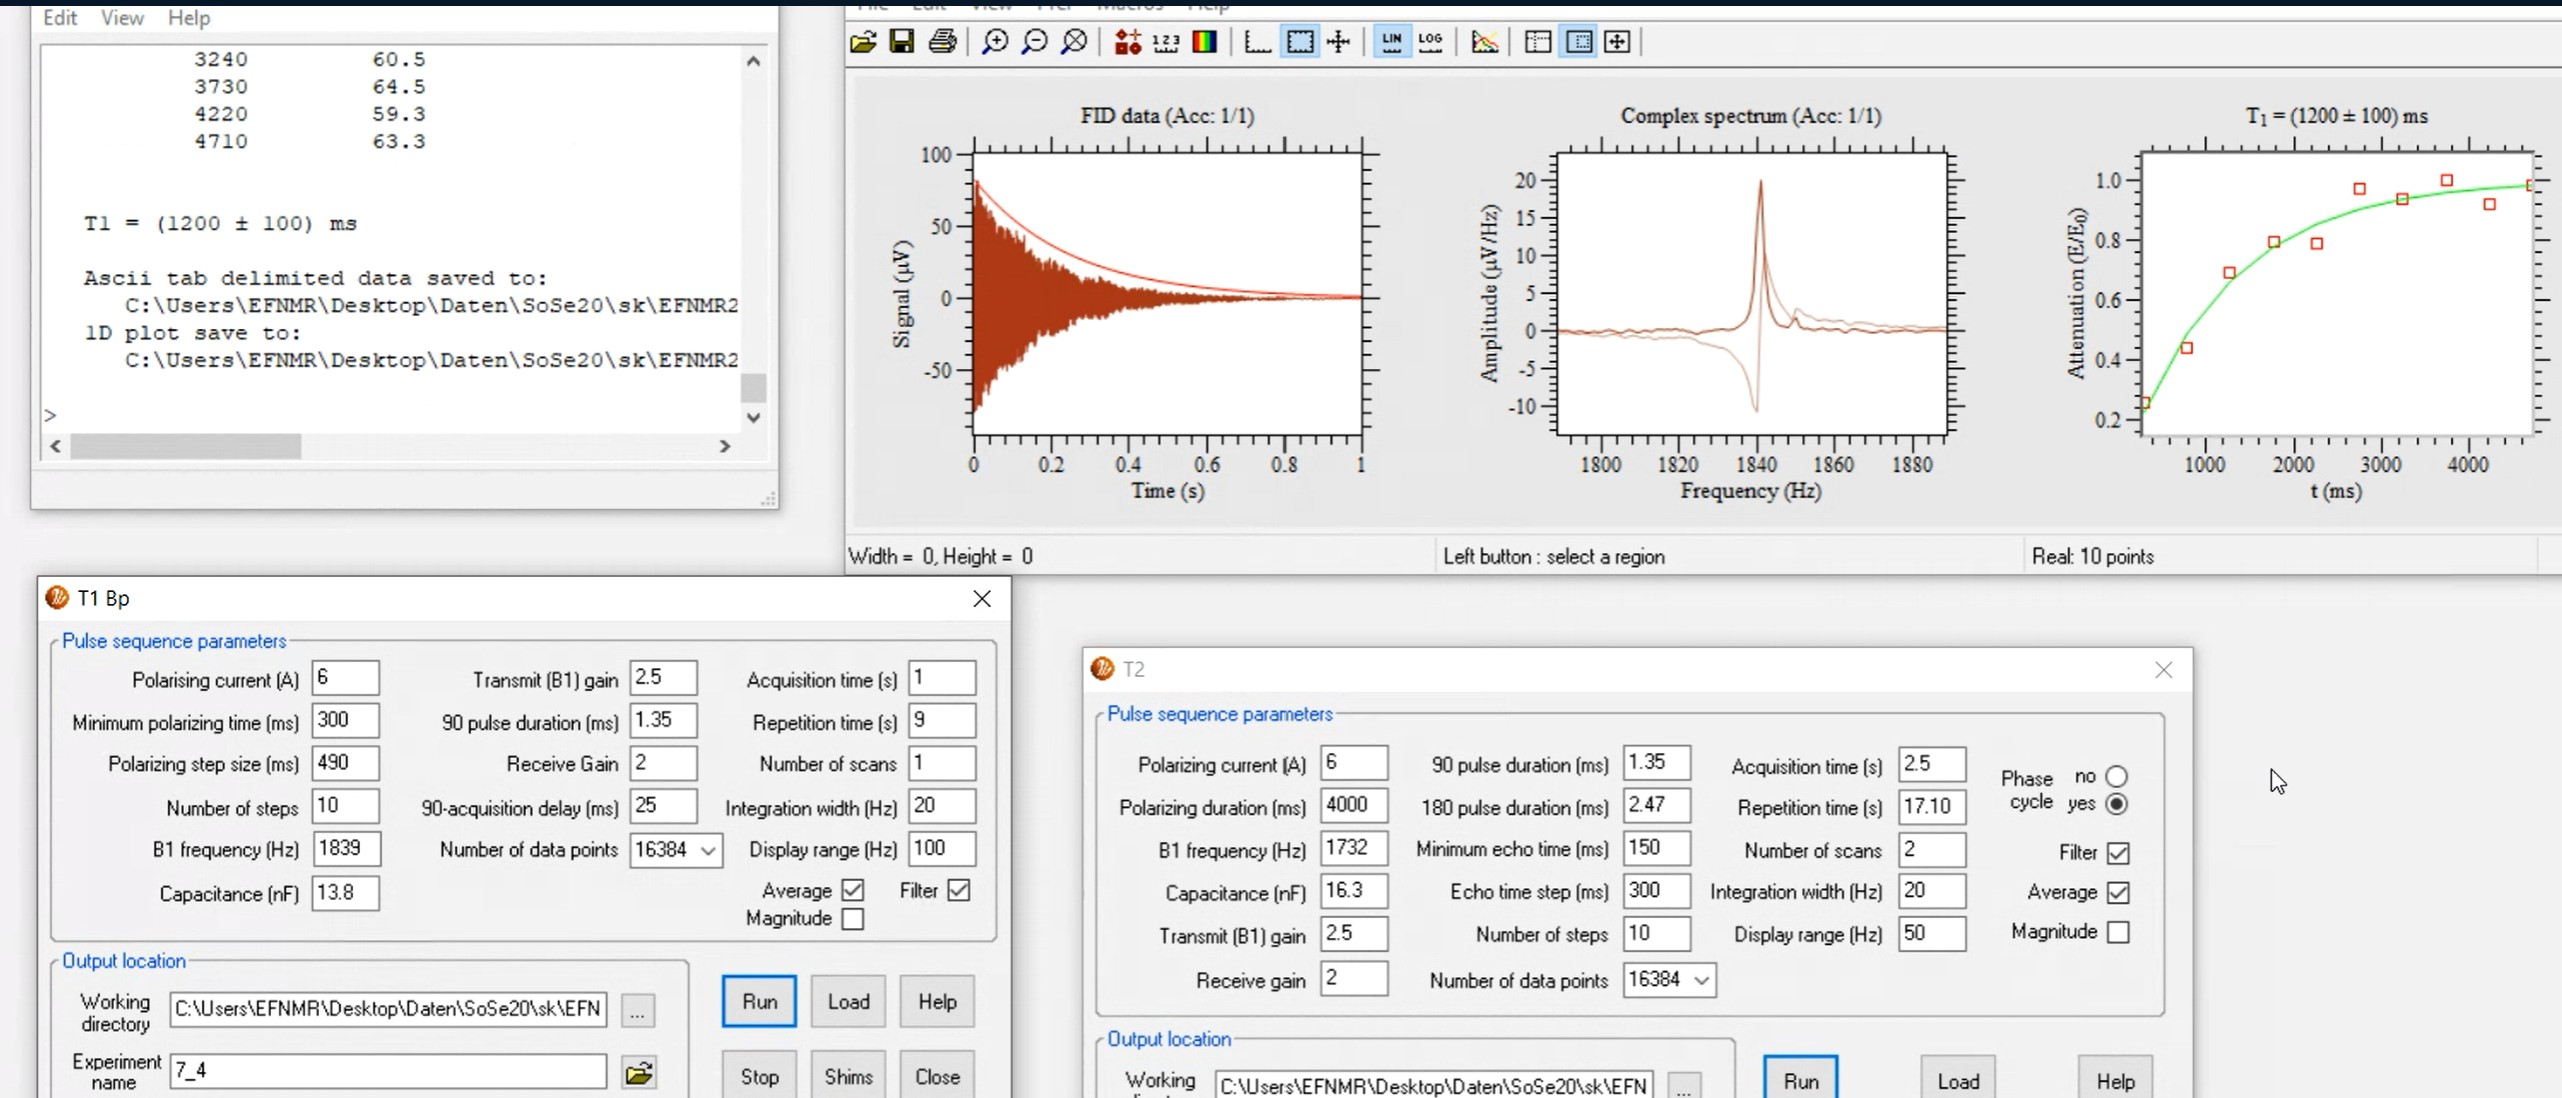
\includegraphics[width = 0.8\textwidth]{Screenshot2/7_4.jpg}
        \caption{7.4}
    \end{figure}

    \begin{figure}[H]
        \centering
        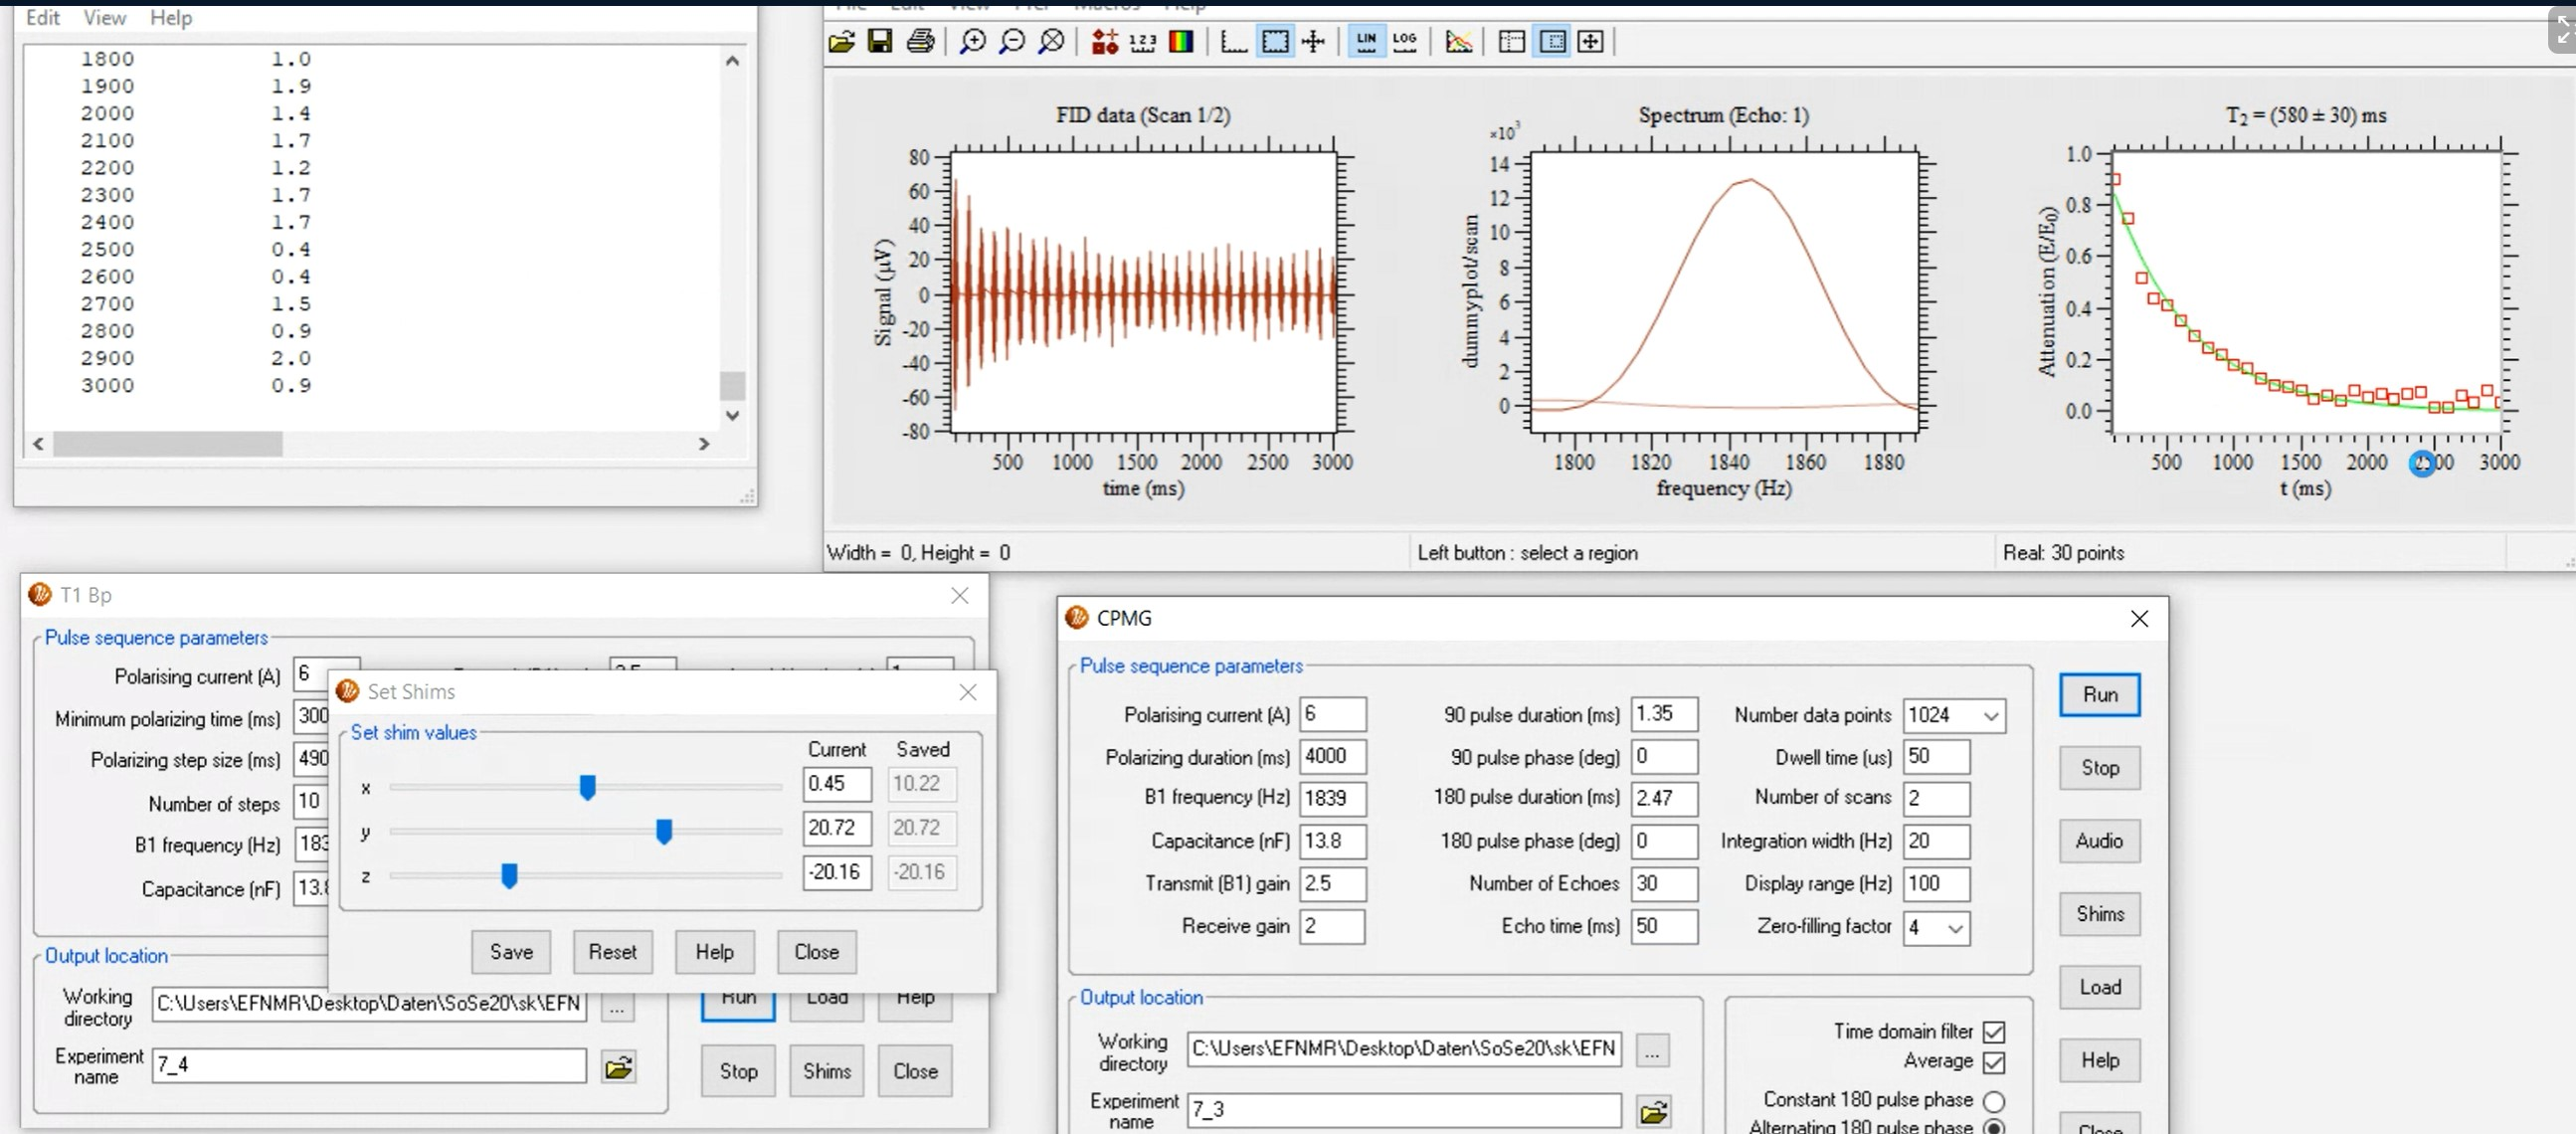
\includegraphics[width = 0.8\textwidth]{Screenshot2/7_3.jpg}
        \caption{7.3}
    \end{figure}

    \begin{figure}[H]
        \centering
        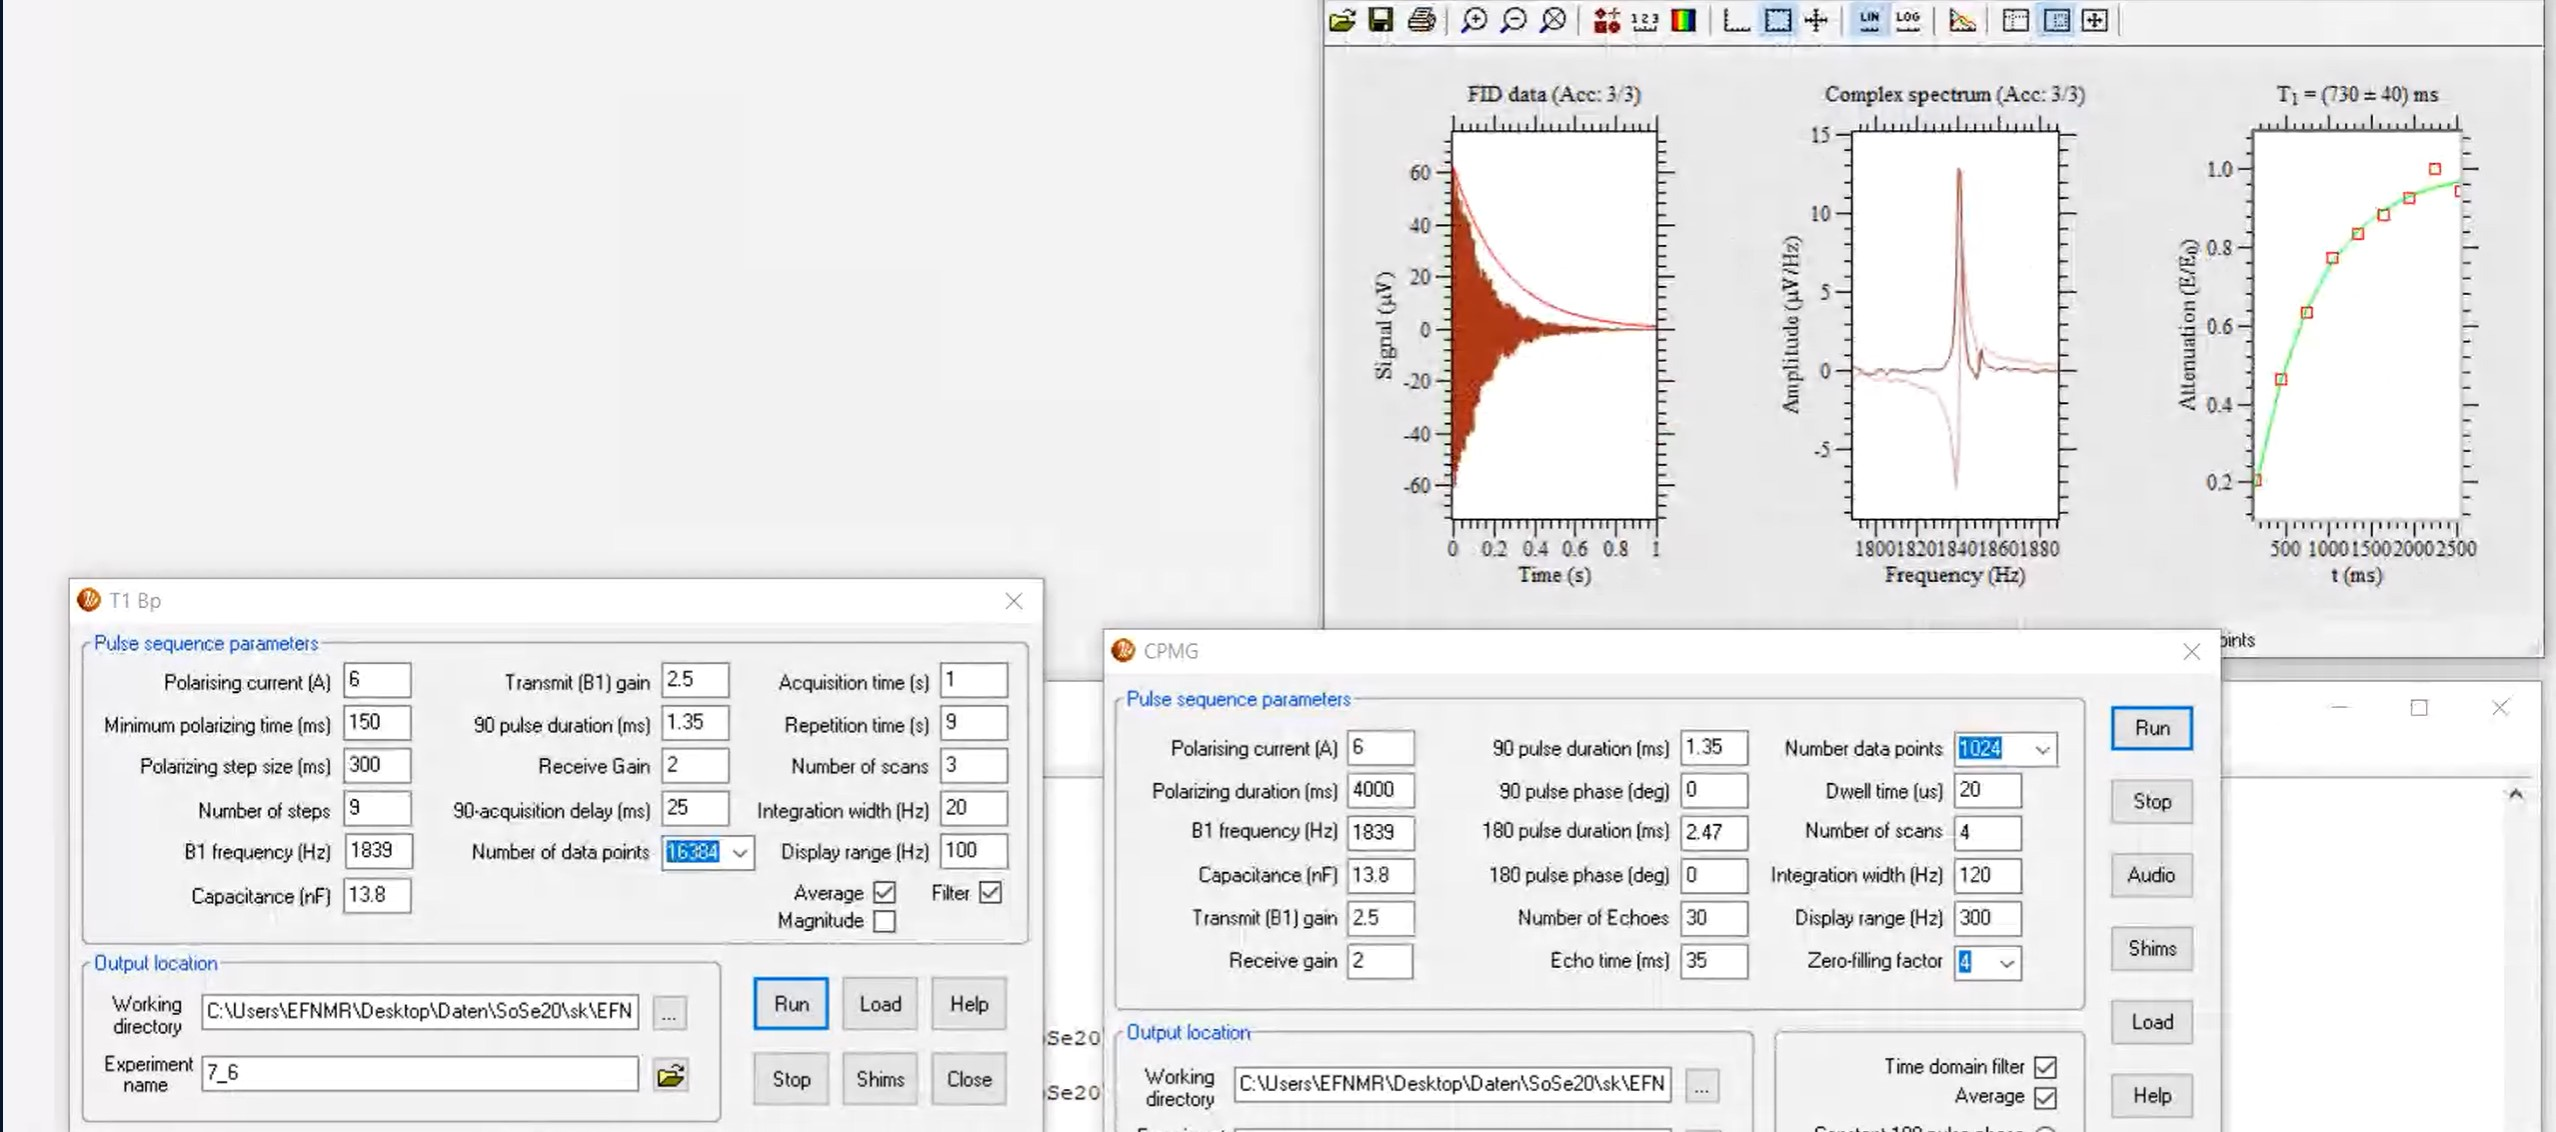
\includegraphics[width = 0.8\textwidth]{Screenshot2/7_6.jpg}
        \caption{7.6}
    \end{figure}

    \begin{figure}[H]
        \centering
        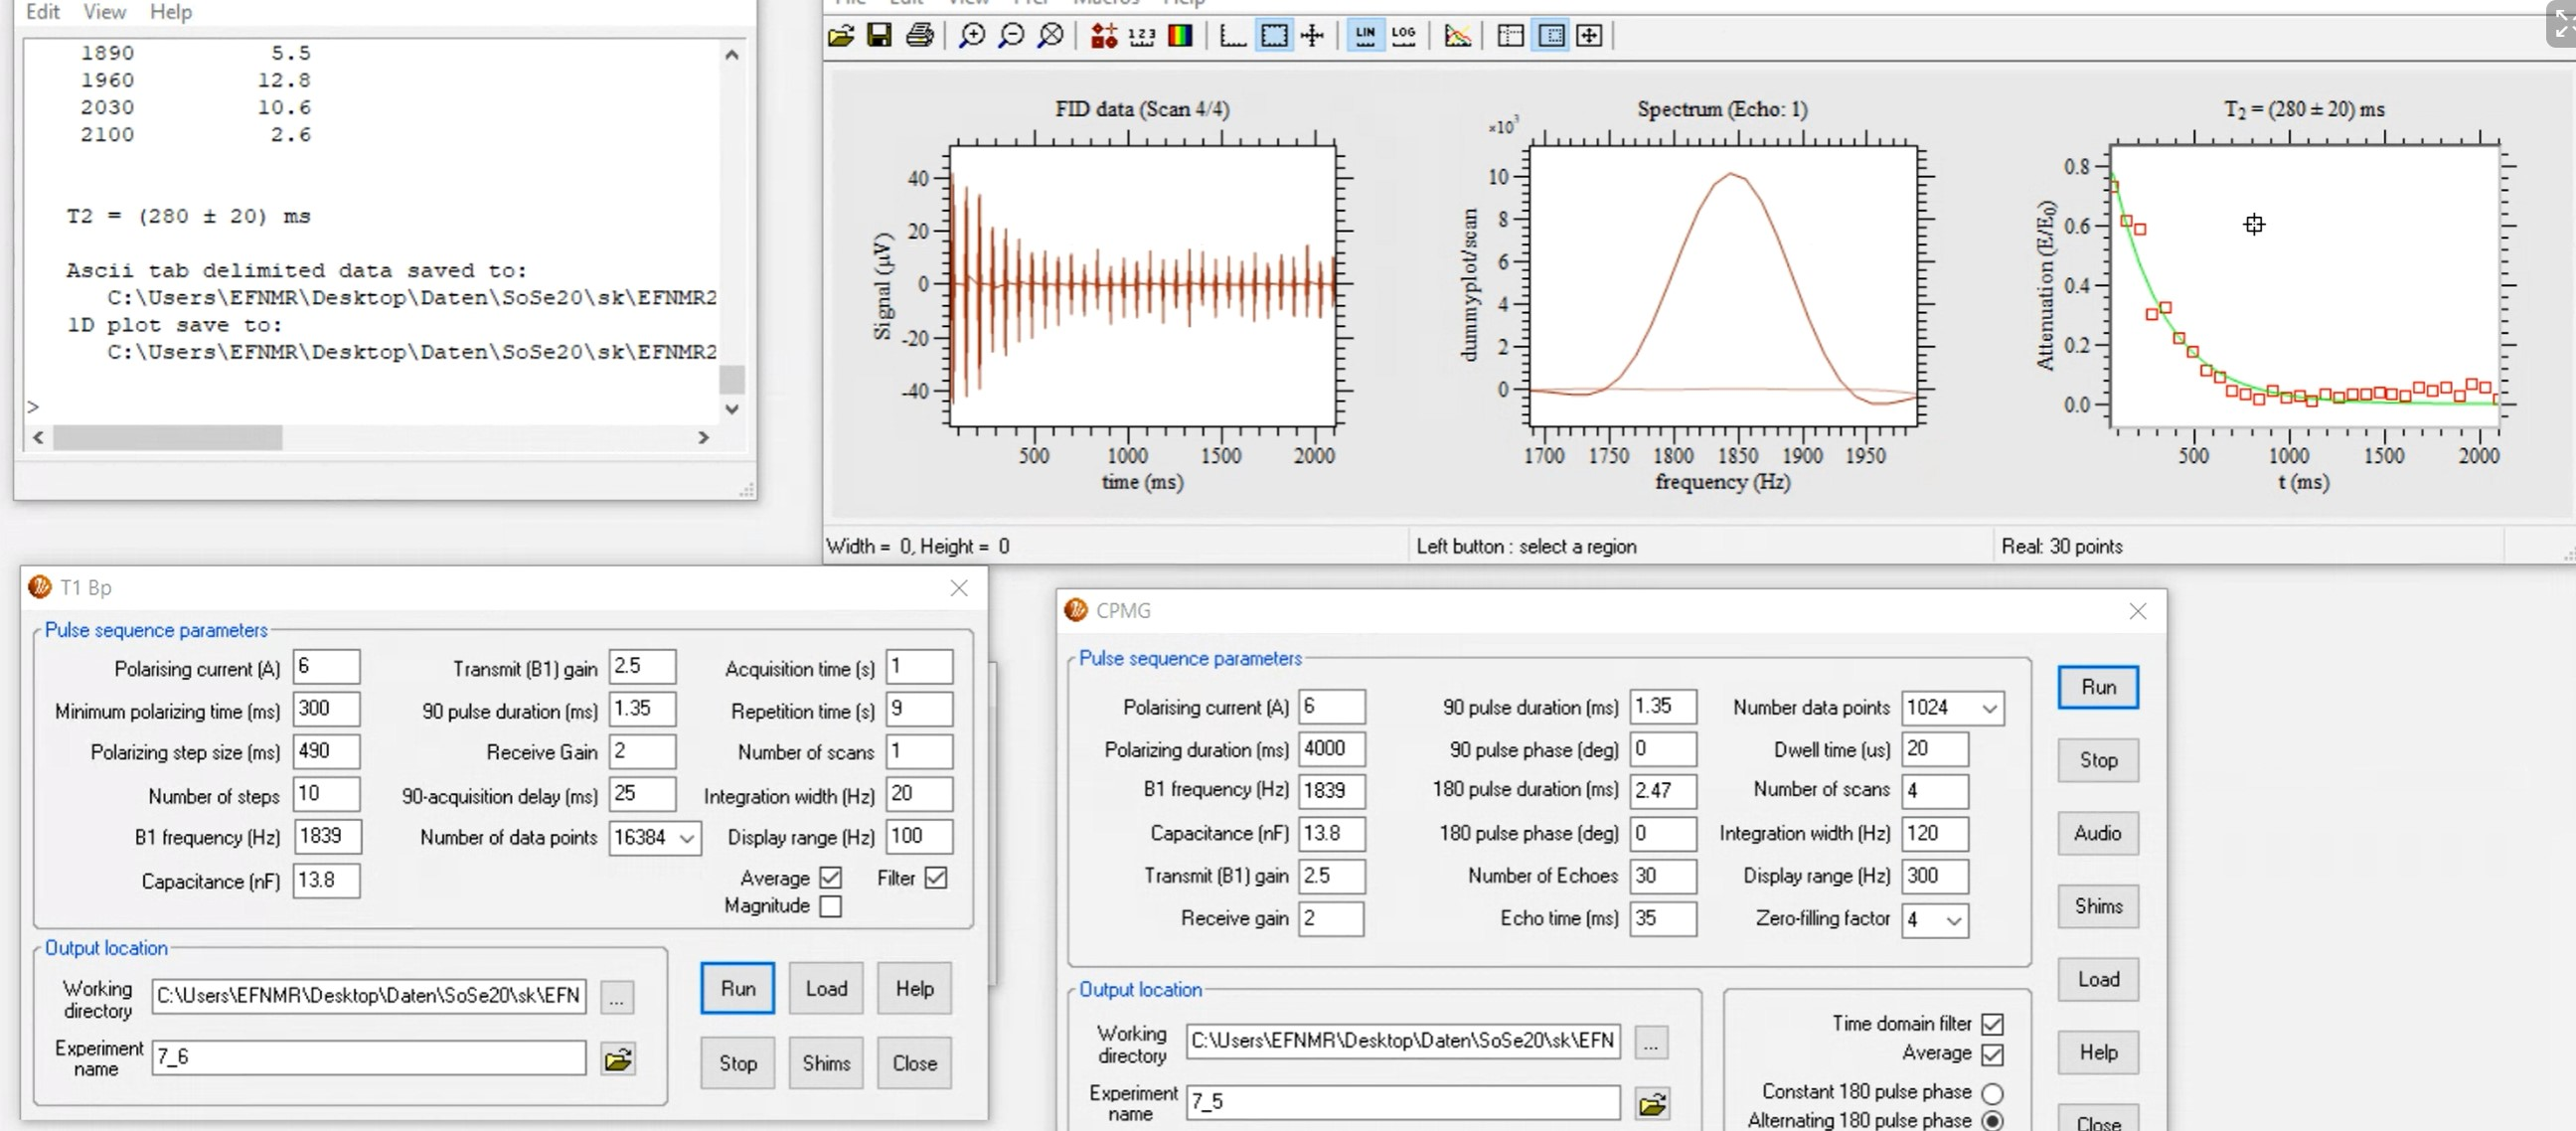
\includegraphics[width = 0.8\textwidth]{Screenshot2/7_5.jpg}
        \caption{7.5}
    \end{figure}



    \subsection{1D Magnetic Resonance Imaging (0.75h)}
    % \begin{itemize}
    %     \item Grundlagen: A one-dimensional image, (often referred to as a profile), of an inherently three-dimensional object, is a projection of the three-dimensional object along a single dimension. \newline
    %     An image along “X” means the gradient will be directed along the x axis of the probe \newline
    %     the alignment of “Z” with the Earth’s field is very important for imaging\newline
    %     \begin{align}
    %         \Delta x = \frac{FOV}{N} \text{nominale Auflösung}
    %     \end{align}
    %     $\Delta x$ Größe einzelner Pixel (Auflösung)

    % \end{itemize}


    \begin{tabular}{ll}

        \textbf{Paramters} &            \\
        
        Shimming values & $x = 10.11$ mA; $y = 20.88$ mA; $z = −20.07$ mA \\
        
        Tuning the probe & Kapazität: 13.8 nF; Polarisationsstrom: 6A;\\
        & Receiver gain: 2; transmit gain (B1): 2.5\\
        & Polaraisationszeit: 4s; Repetition time: 15s; \\
        & Number of scans: 1\\
        
        Setting B1 to lamor frequency &    1837 Hz \\
        
        duration 90 and 180 pulse & 90 Grad: 1.35 ms; 180 Grad: 2.7ms \\
        \end{tabular}  
        
        \vspace{1cm}

\begin{tabular}{ll}
    \textbf{Durchführung} & \\

    8.1 & Setzte Parameter in ''Common Parameters''  \\

        &  auf unsere Werte \\

    9.1 & GradEchoImaging: Wähle  ''1D'' in Image parameters;  \\

        & Wähle ''X''-Achse; FOV Matrix size startwert 32; FOV: 200mm \\

    9.2 & Wähle Anfangswerte für water tube: phase gradient duration = 270 ms \textbf{(auf 80ms)},  \\

        & band width 64 Hz, number of scans = 4; G = 7.5 $\frac{\mu T}{m}$ \\

        & echo time calculated: 0.54s with acquisition delay 0.02s \\

    9.3 & GradEchoImaging: Wähle  ''1D'' in Image parameters;  \\

        & Wähle ''Y''-Achse; FOV Matrix size startwert 32; FOV: 200mm \\

    9.4 & Wähle Anfangswerte für water tube: phase gradient duration = 270 ms,  \\

        & band width 64 Hz (\textbf{auf 32 Hz}), number of scans = 4; G = 7.5 $\frac{\mu T}{m}$ \\

        & echo time calculated: 0.54s with acquisition delay 0.02s \\

    9.5 &  Um mal eine und mal die andere Röhre zu sehen, \\
    & muss die echo time oder polarisation time varriert werden \\

\end{tabular}  

Auf dem Magnitudebild ist ein Peak bei ca. 1850. Dieser kommt durch die getaktete Steckdose. 
Schaue noise an, wo die Peaks alle 50 Hz groß sind

\begin{figure}[H]
    \centering
    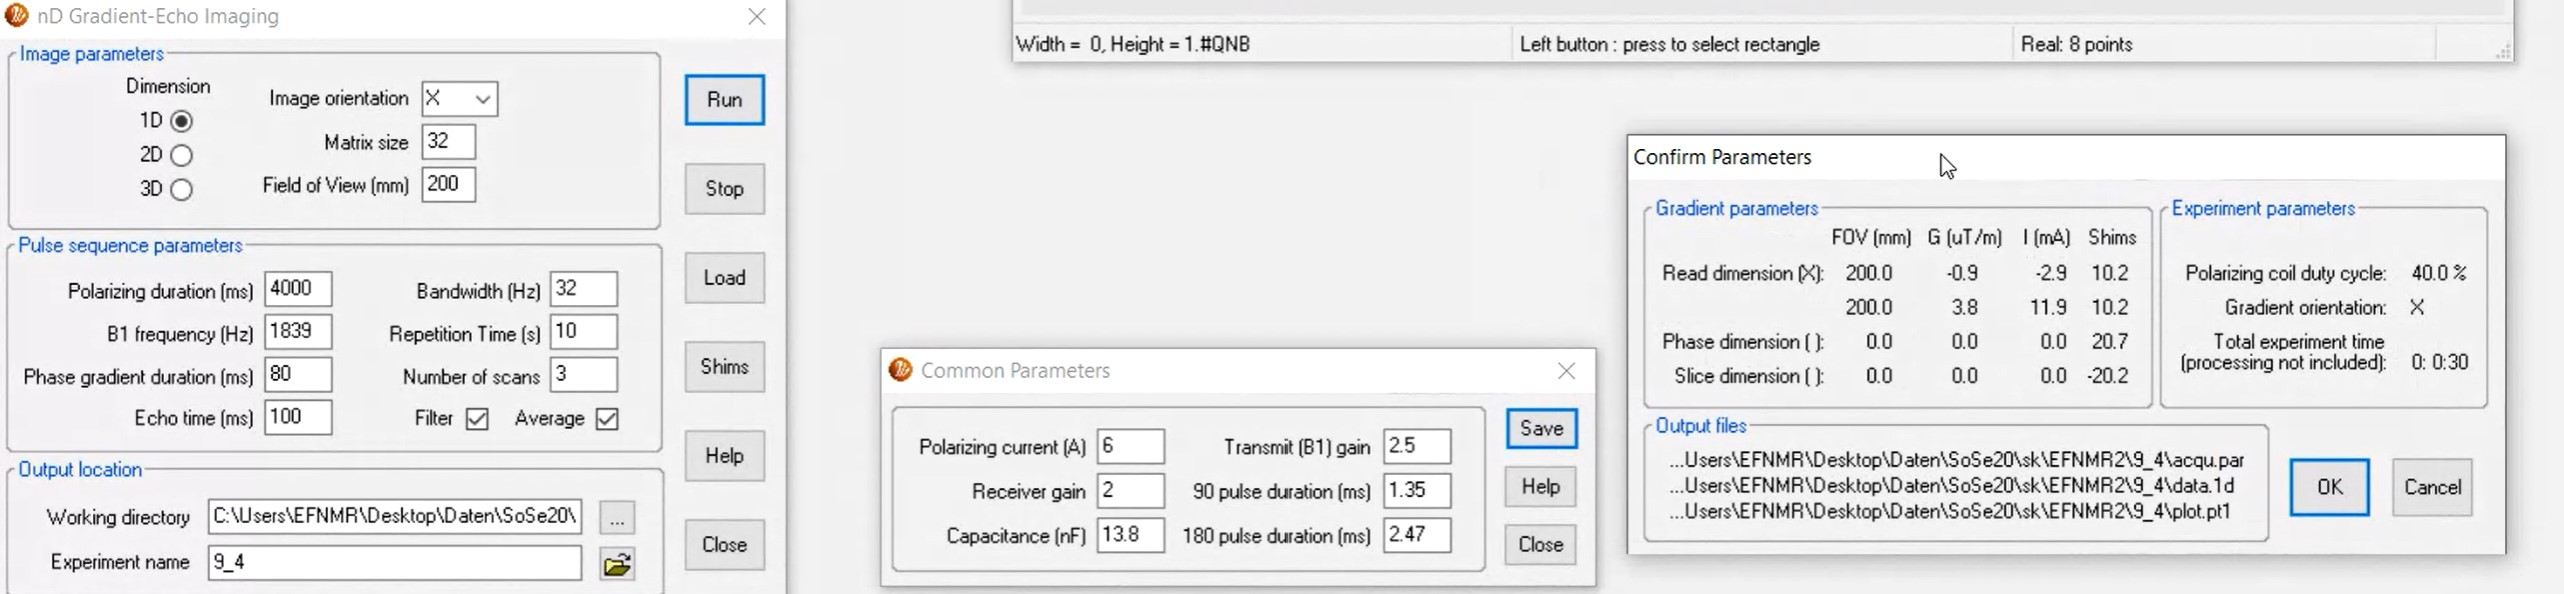
\includegraphics[width = 0.8\textwidth]{Screenshot2/9_2Messwerte.jpg}
\end{figure}

\begin{figure}[H]
    \centering
    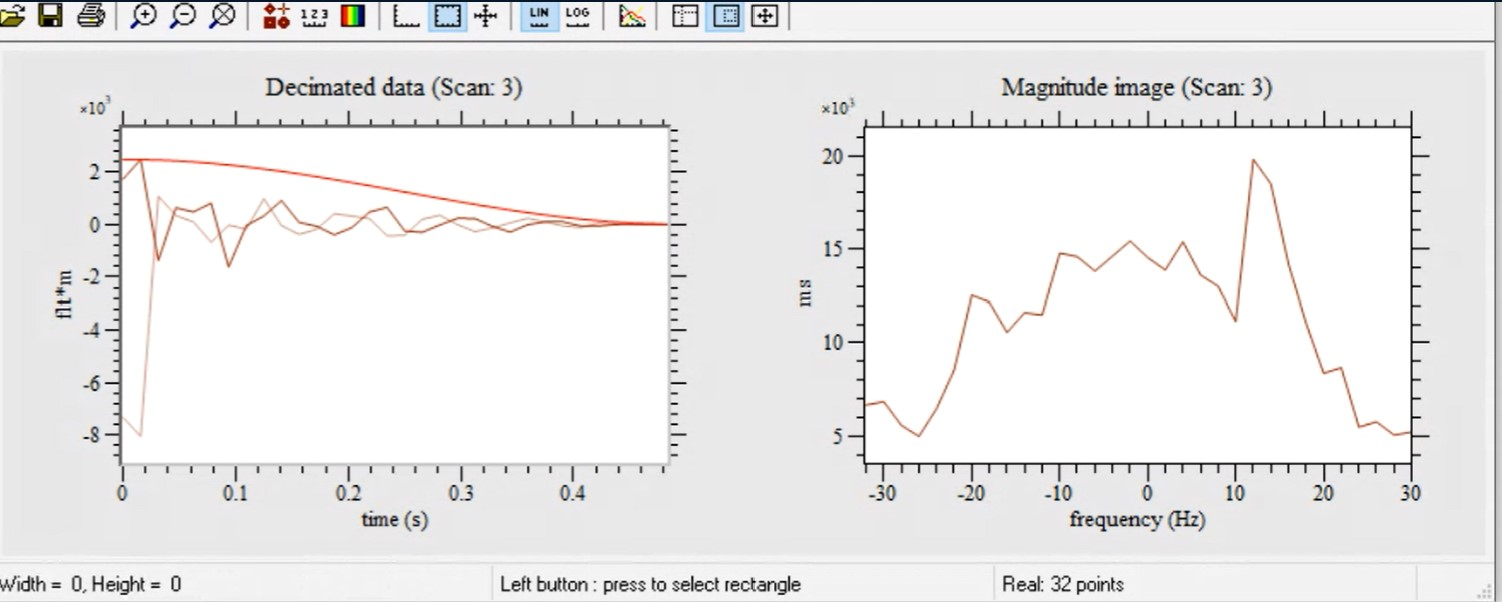
\includegraphics[width = 0.8\textwidth]{Screenshot2/9_2Messergebnisse.jpg}
\end{figure}


\begin{figure}[H]
    \centering
    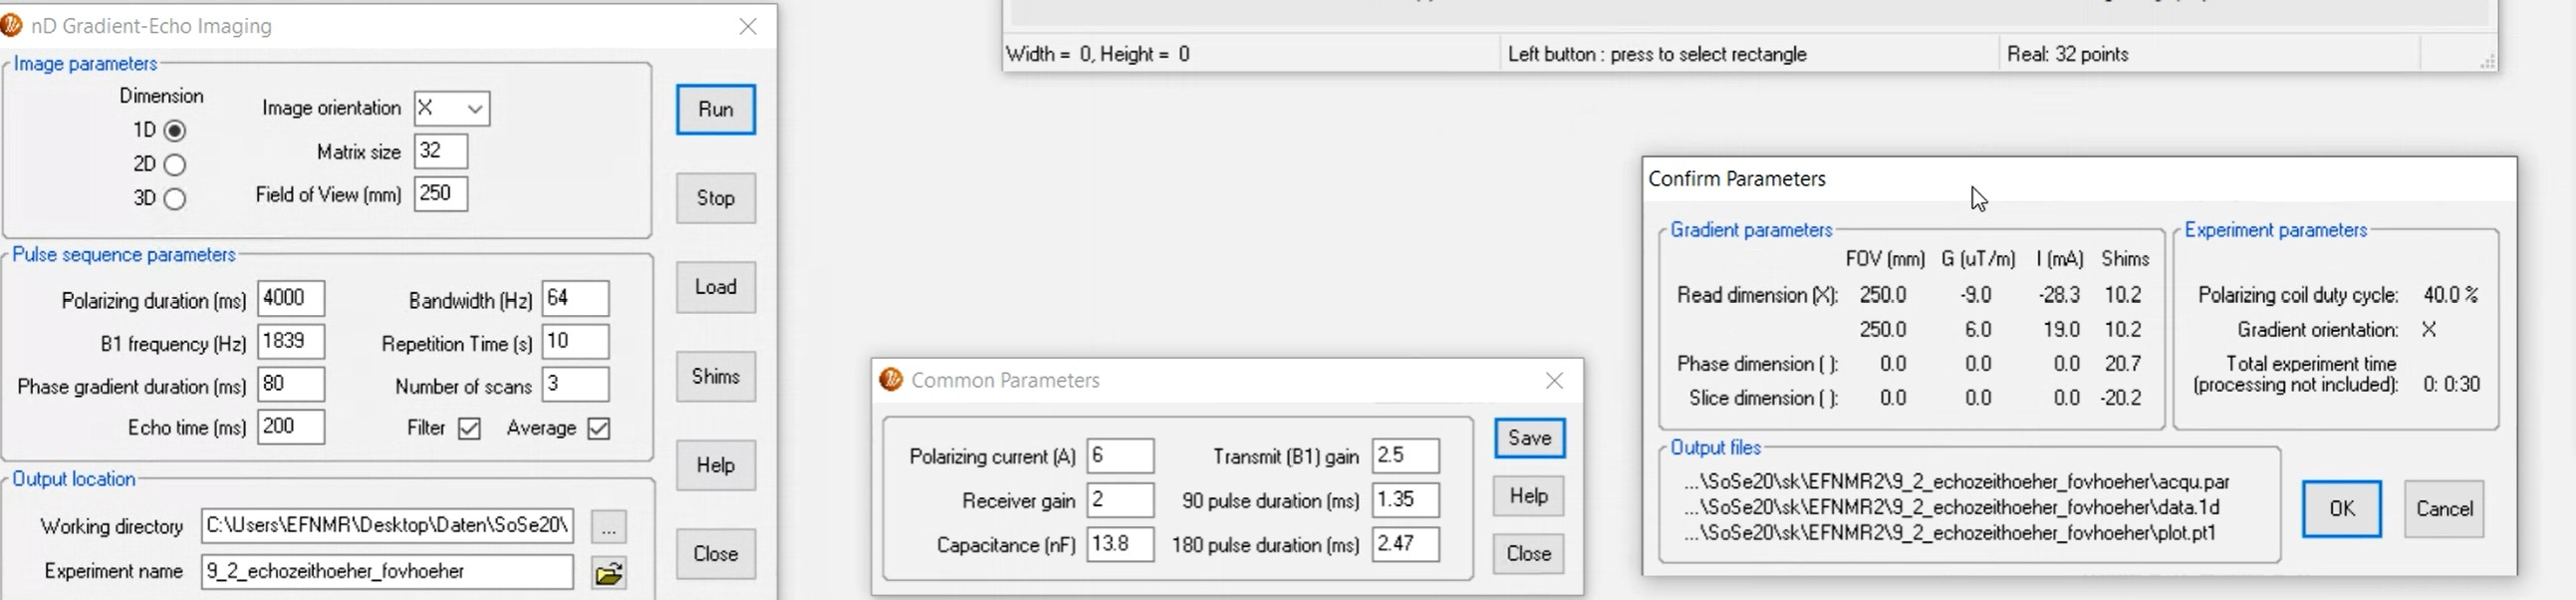
\includegraphics[width = 0.8\textwidth]{Screenshot2/9_2_Messwerte_echozeithoeher_fovhoeher.jpg}
\end{figure}

\begin{figure}[H]
    \centering
    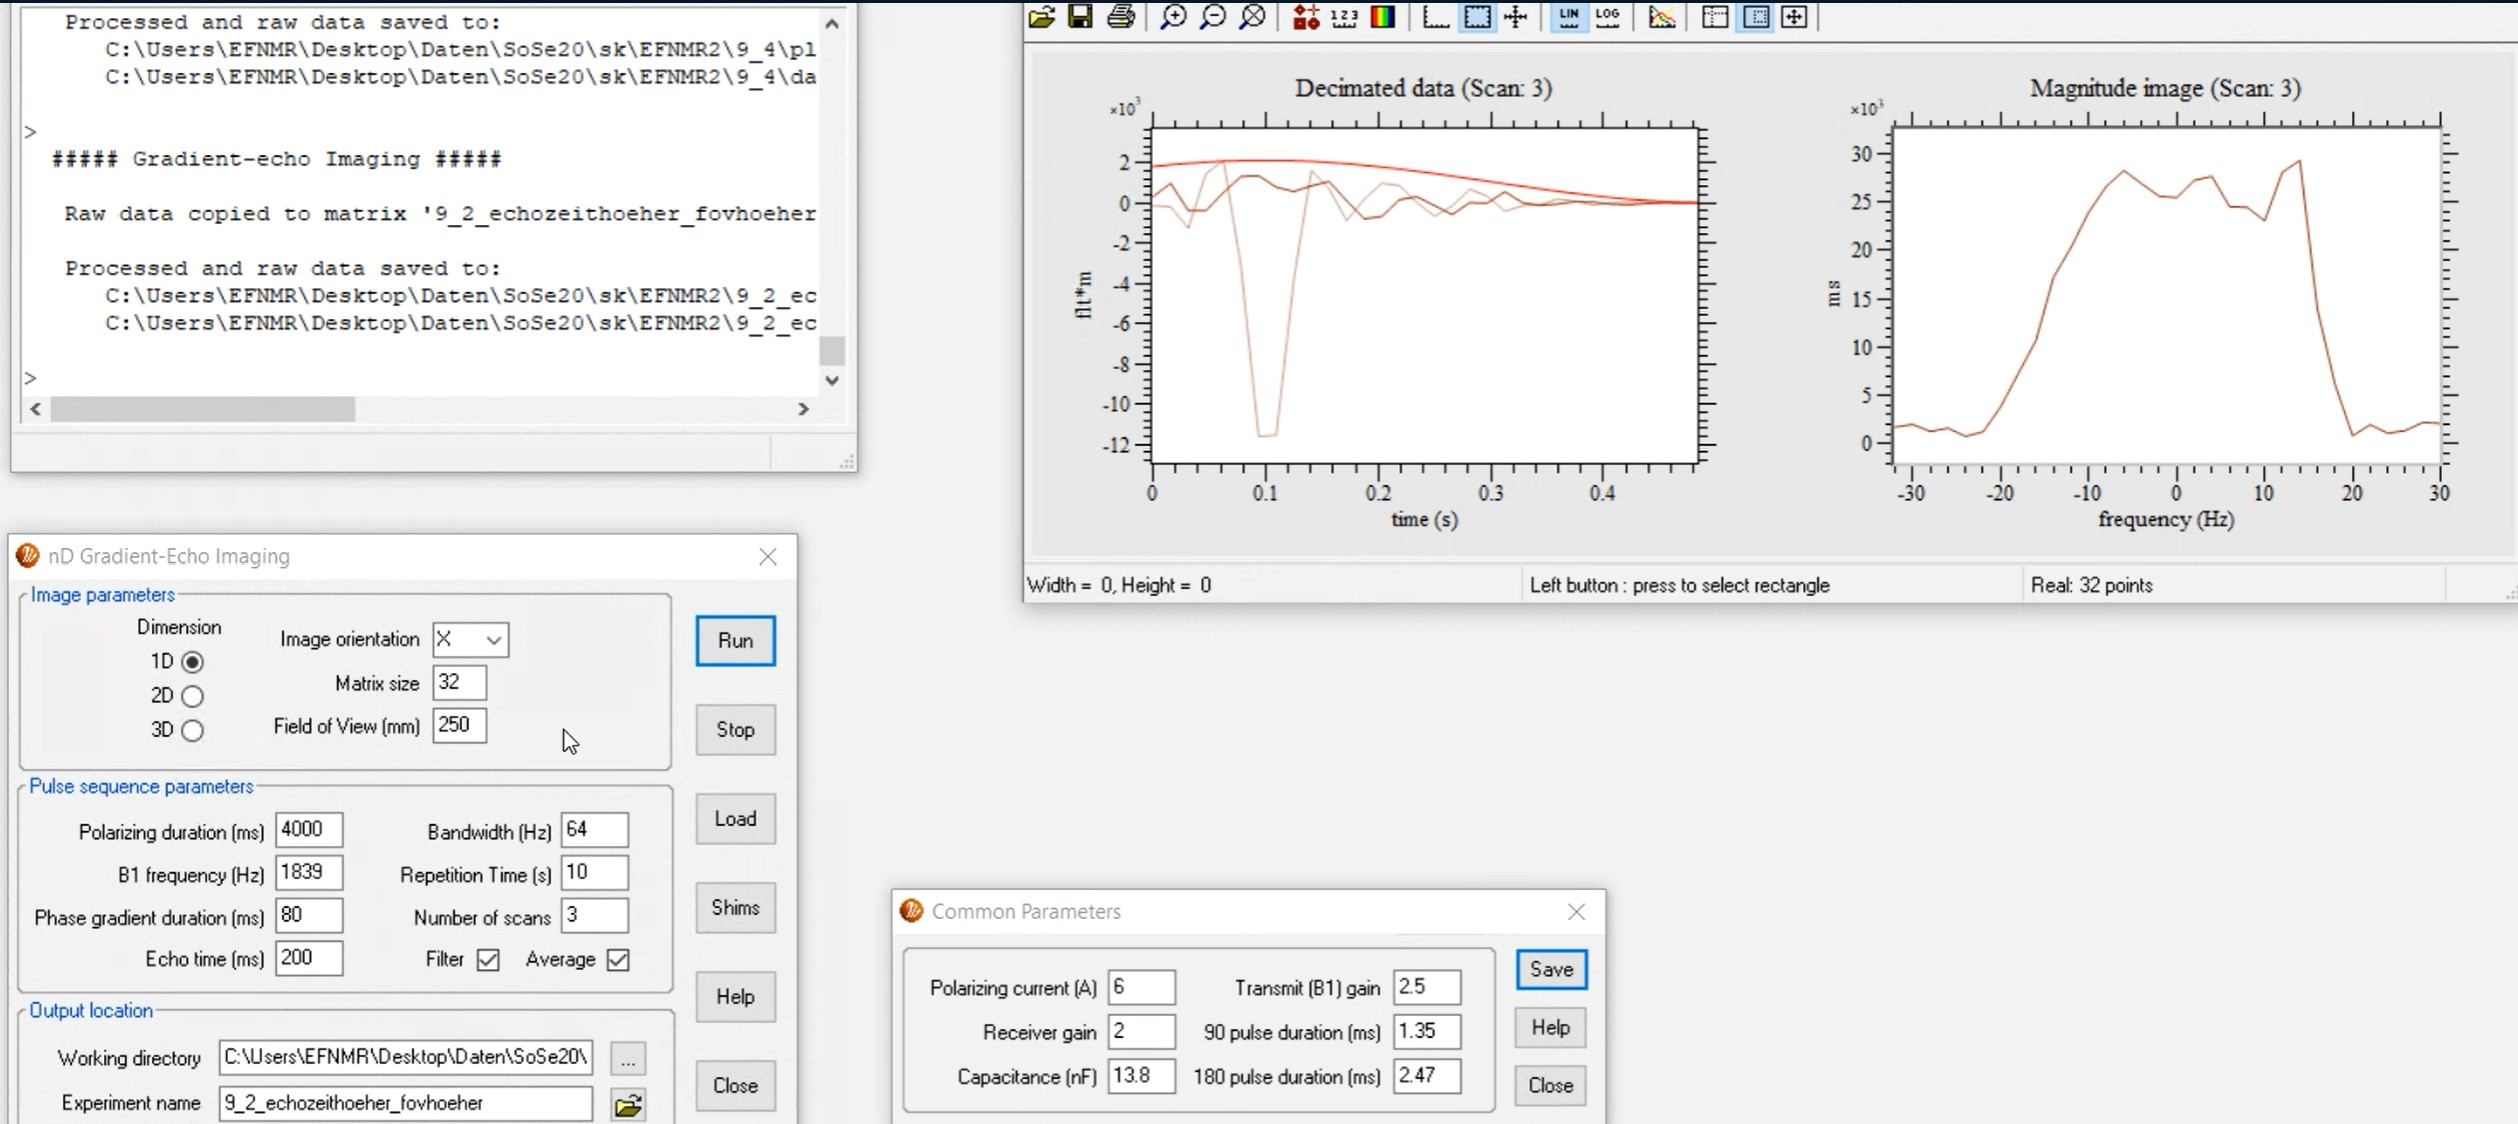
\includegraphics[width = 0.8\textwidth]{Screenshot2/9_2_Messergebnisse_echozeithoeher_fovhoeher.jpg}
\end{figure}

\begin{figure}[H]
    \centering
    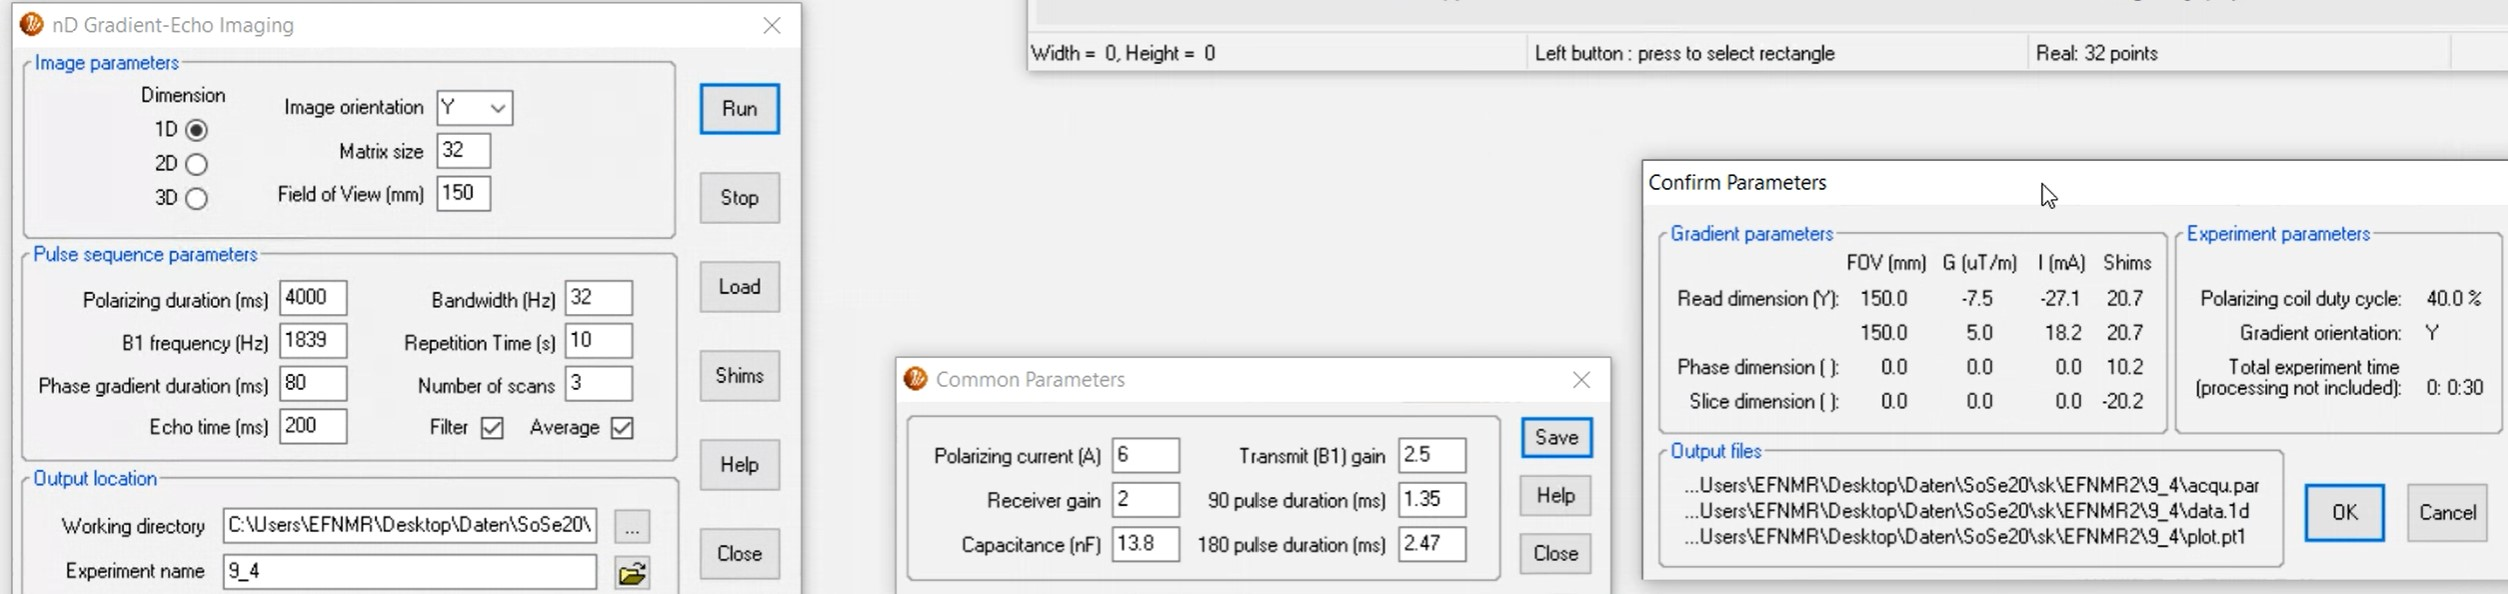
\includegraphics[width = 0.8\textwidth]{Screenshot2/9_4Messwerte.jpg}
\end{figure}

\begin{figure}[H]
    \centering
    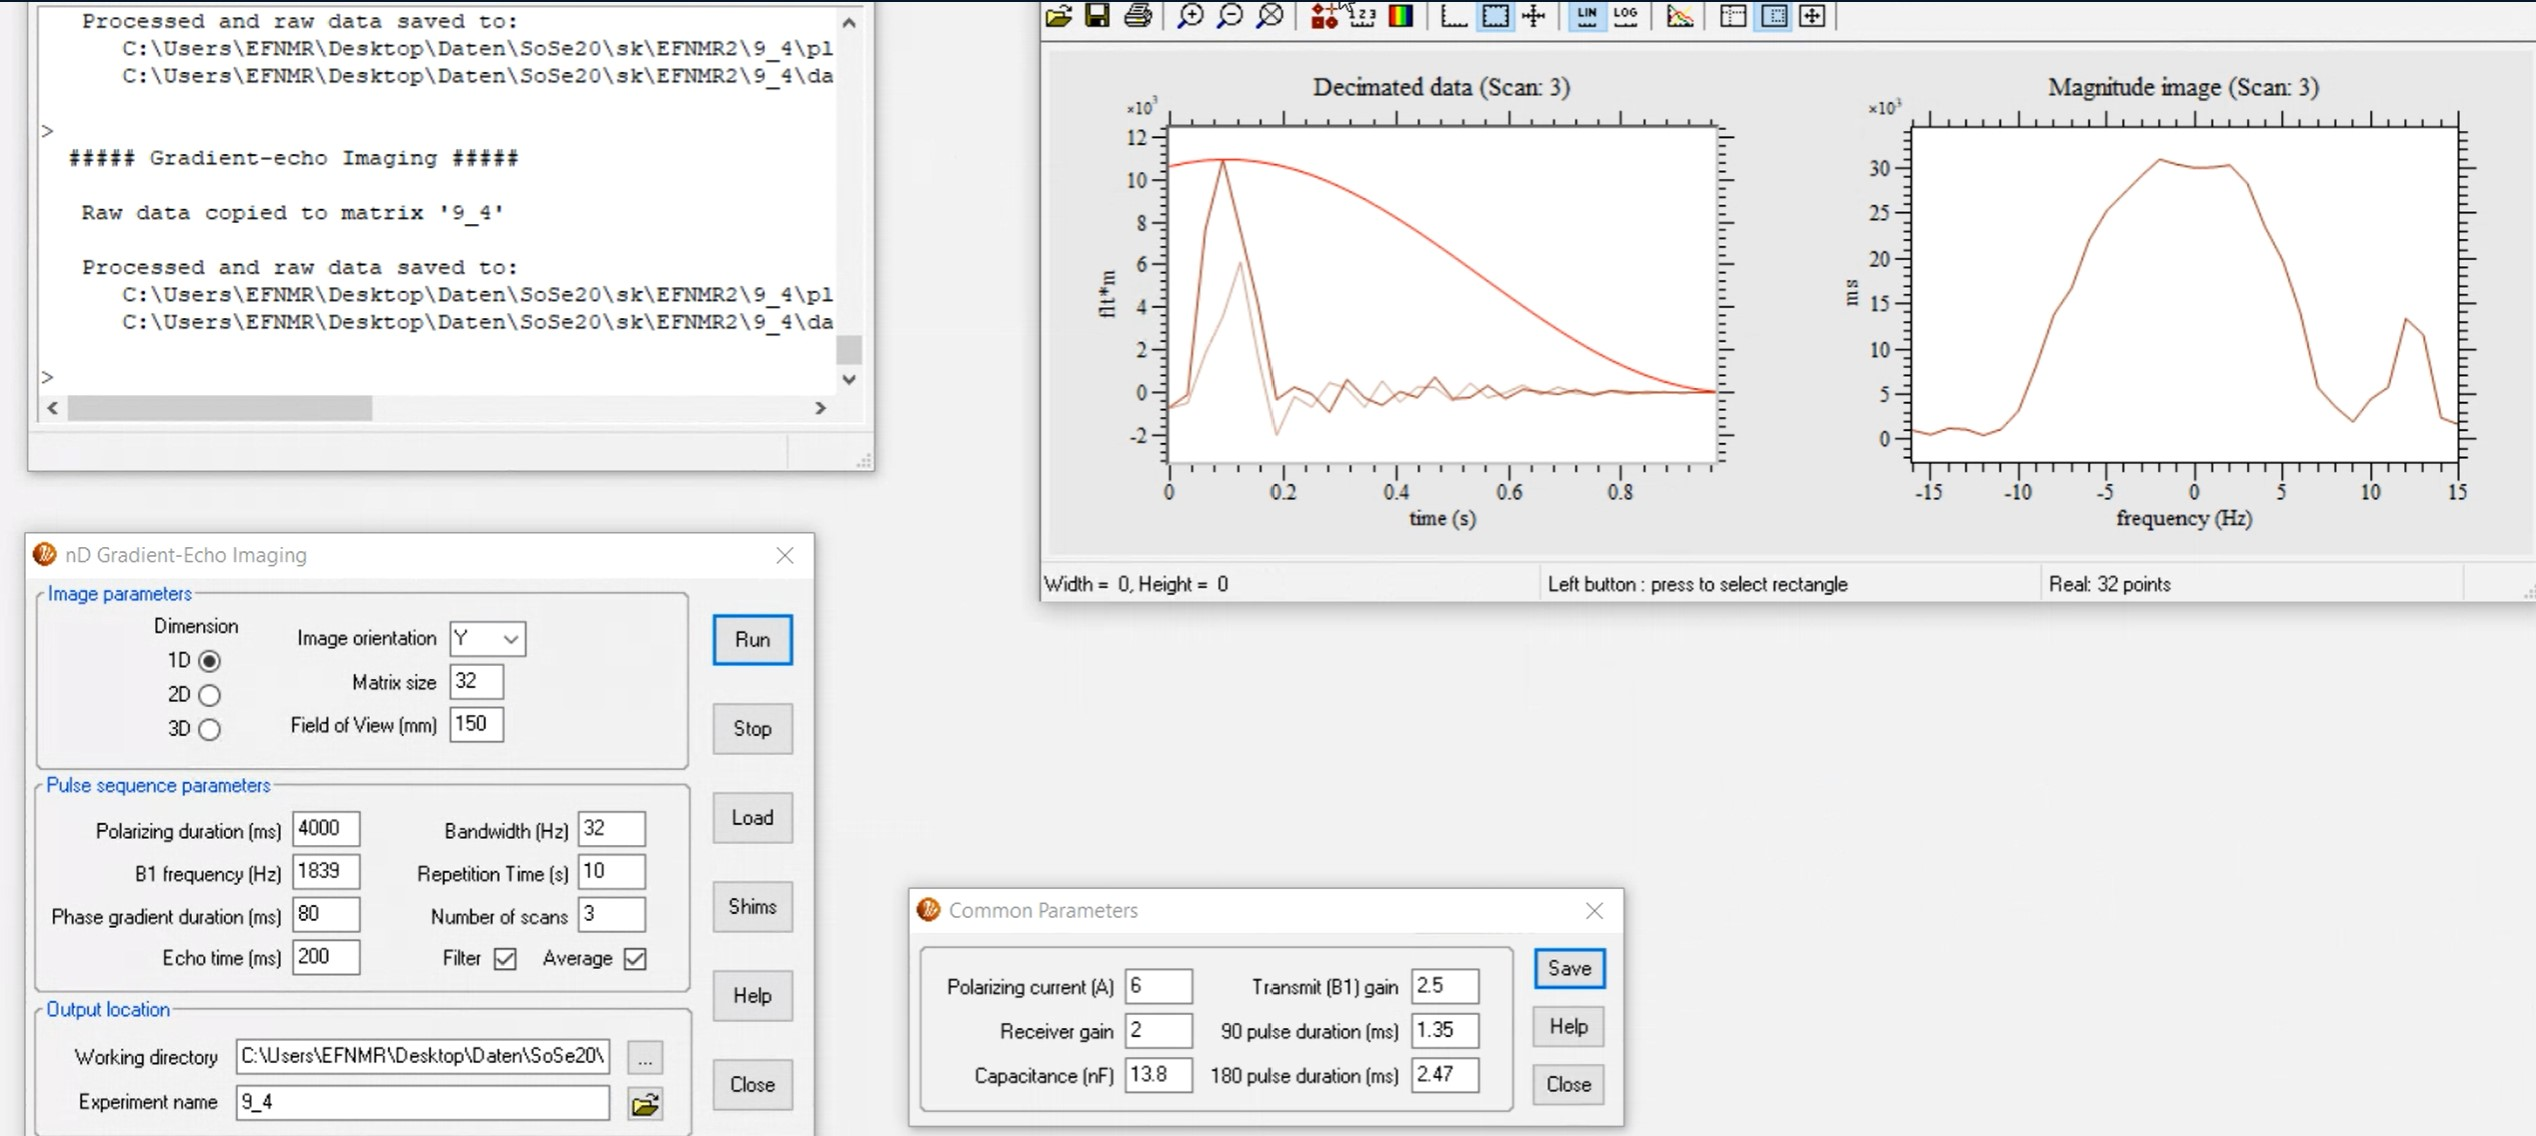
\includegraphics[width = 0.8\textwidth]{Screenshot2/9_4Messergebnisse.jpg}
\end{figure}

\begin{figure}[H]
    \centering
    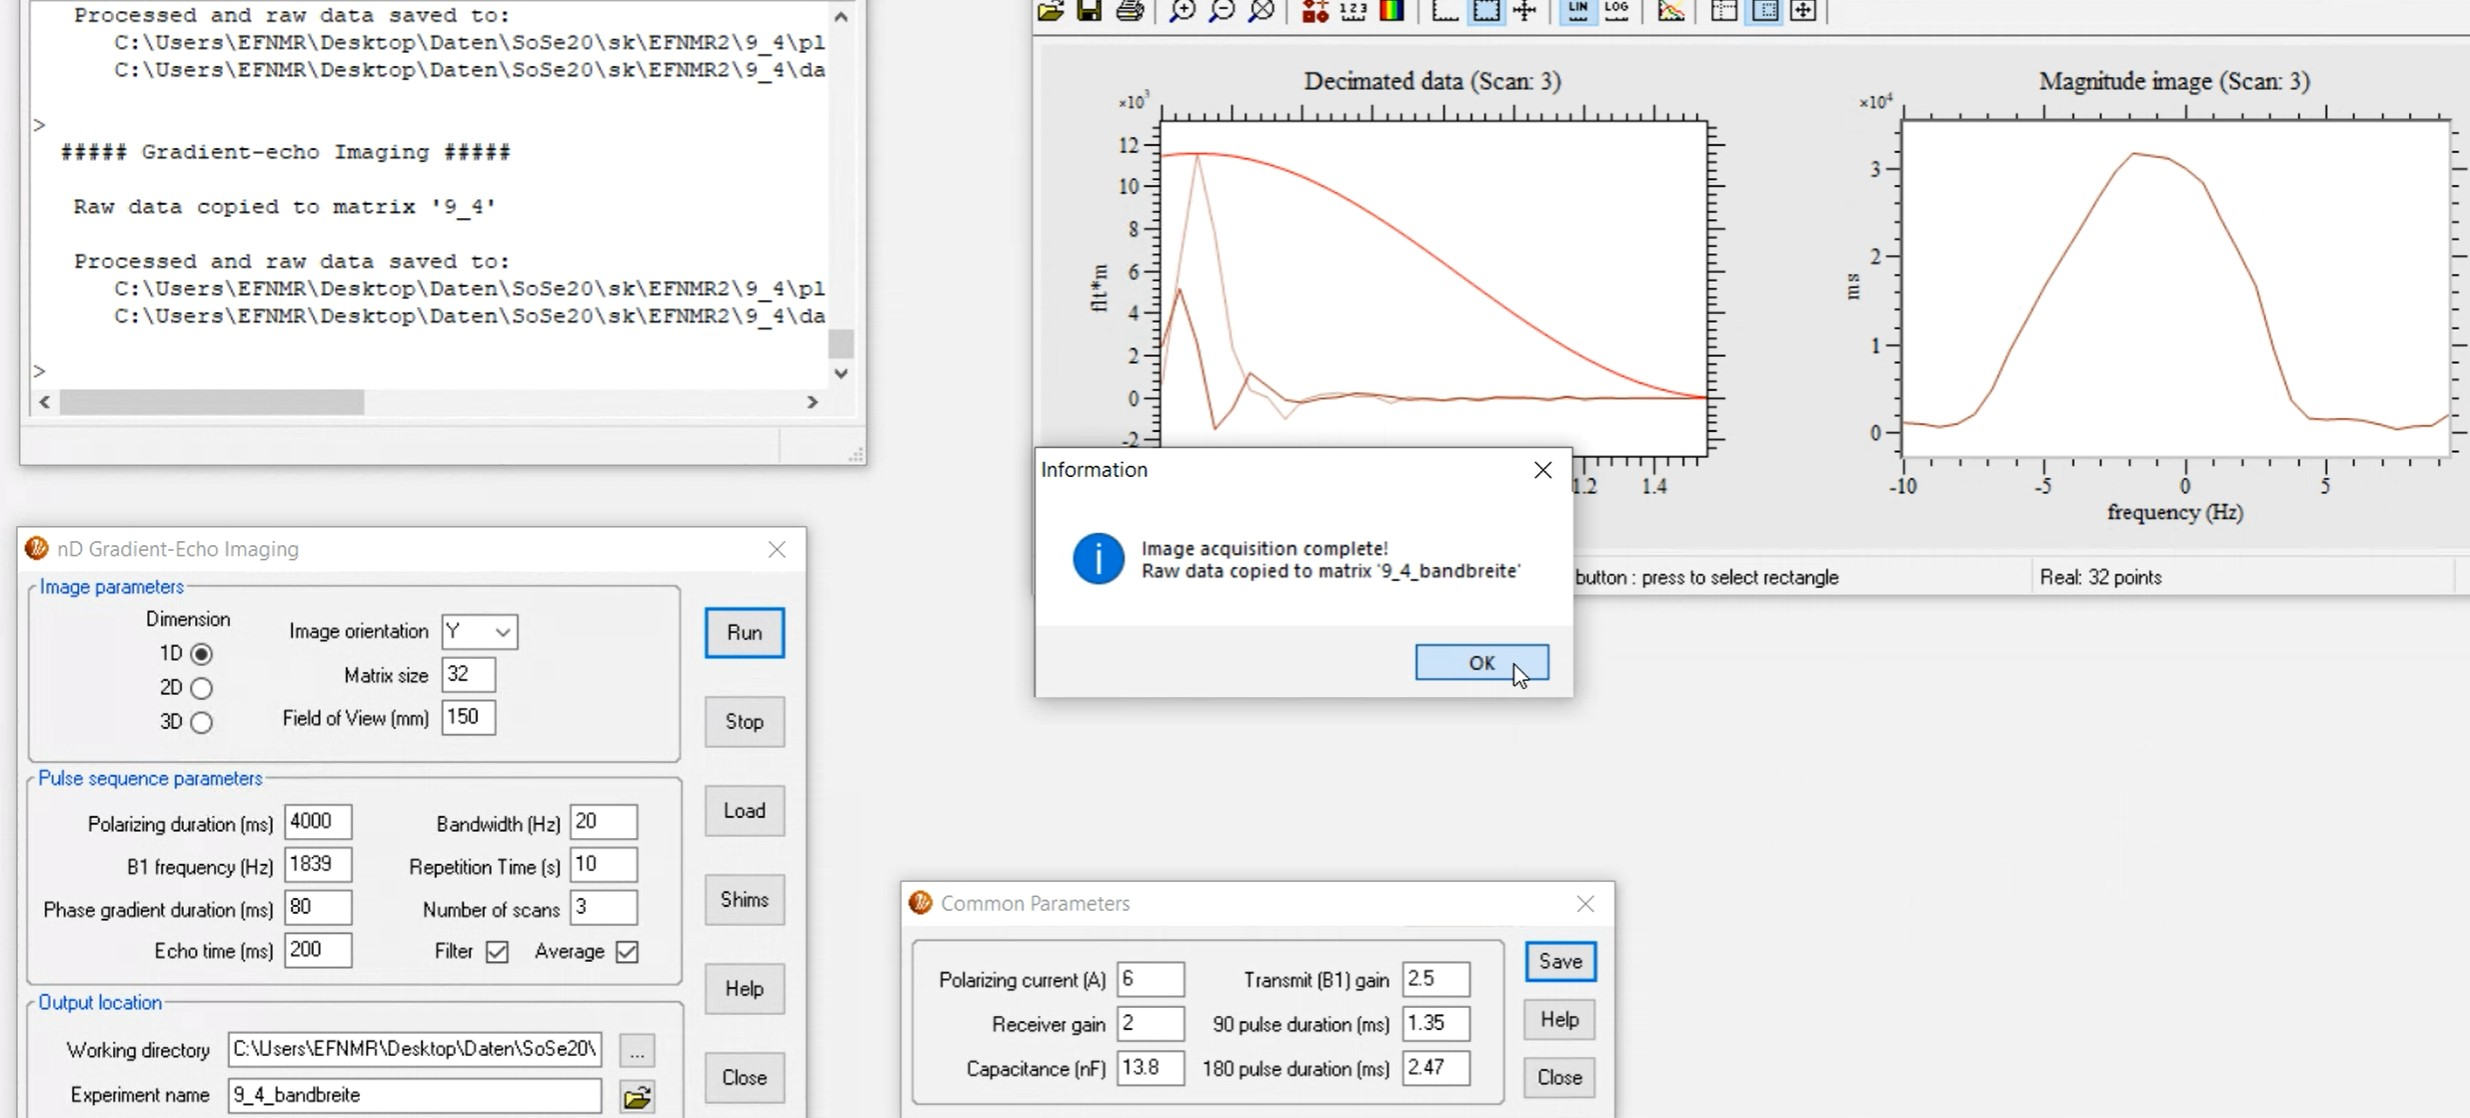
\includegraphics[width = 0.8\textwidth]{Screenshot2/9_4_bandbreite.jpg}
\end{figure}


\subsection{J-Kopplung (1h)}
% \begin{itemize}
%     \item Grundlagen:  in the Earth’s field the absolute frequency difference between hetero-nuclei is very small due to the weak nature of the Earth’s magnetic field. This allows for simultaneous observation of NMR signals from
%     hetero-nuclei such as 1H and 19F\newline
%     Earth’s field NMR is particularly well suited to observing purely J coupled spectra for two reasons. First J coupling constants are independent of field (J coupling splitting of 7 Hz in a 700 MHz spectrometer (i.e. 0.01 ppm) has the same 7 Hz splitting in an Earth’s field system (i.e. ~ 3000 ppm)). Second, the high homogeneity of the Earth’s field permits an absolute resolution in Hz which is on par or in some cases even better than that oflaboratory instruments.
%     \item Durchführung:
% \end{itemize}


    \begin{tabular}{ll}

        \textbf{Paramters} &            \\
        
        Shimming values & $x = 10.11$ mA; $y = 20.88$ mA; $z = −20.07$ mA \\
        
        Tuning the probe & Kapazität: 13.8 nF; Polarisationsstrom: 6A;\\
        & Receiver gain: 2; transmit gain (B1): 2.5\\
        & Polaraisationszeit: 4s; Repetition time: 15s; \\
        & Number of scans: 1\\
        
        Setting B1 to lamor frequency &    1837 Hz \\
        
        duration 90 and 180 pulse & 90 Grad: 1.35 ms; 180 Grad: 2.7ms \\
    \end{tabular} 

    \vspace{1cm}


    \begin{figure}[H]
        \centering
        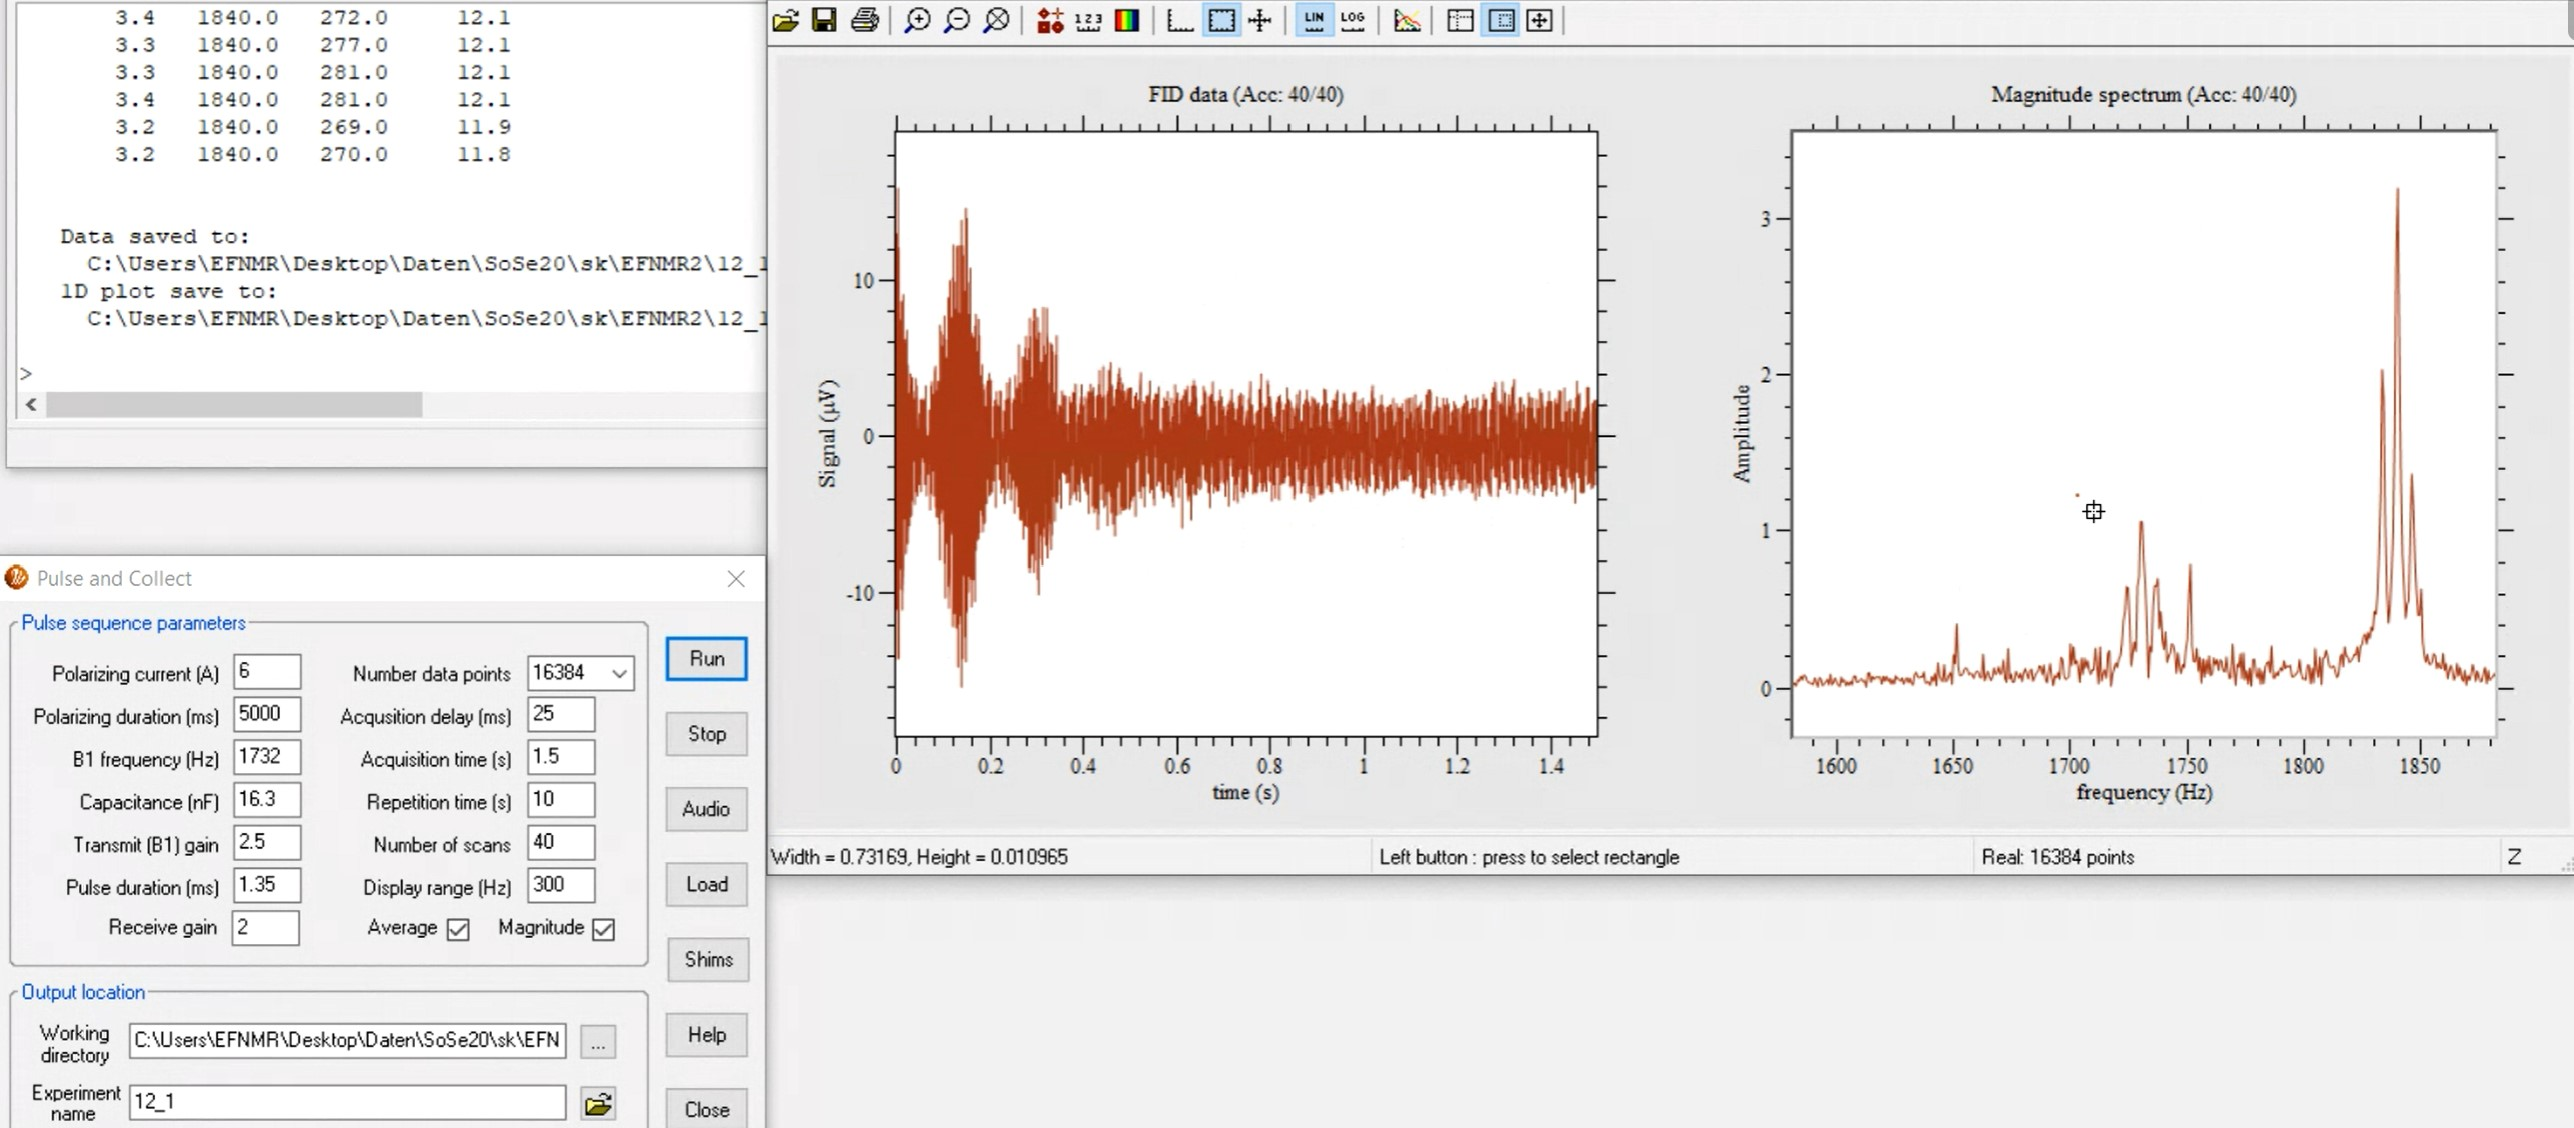
\includegraphics[width=0.8\textwidth]{Screenshot2/12_1rauschen.jpg}
        \caption{Test für JKopplung; 12.1großes Rauschen}
    \end{figure}

    \begin{figure}[H]
        \centering
        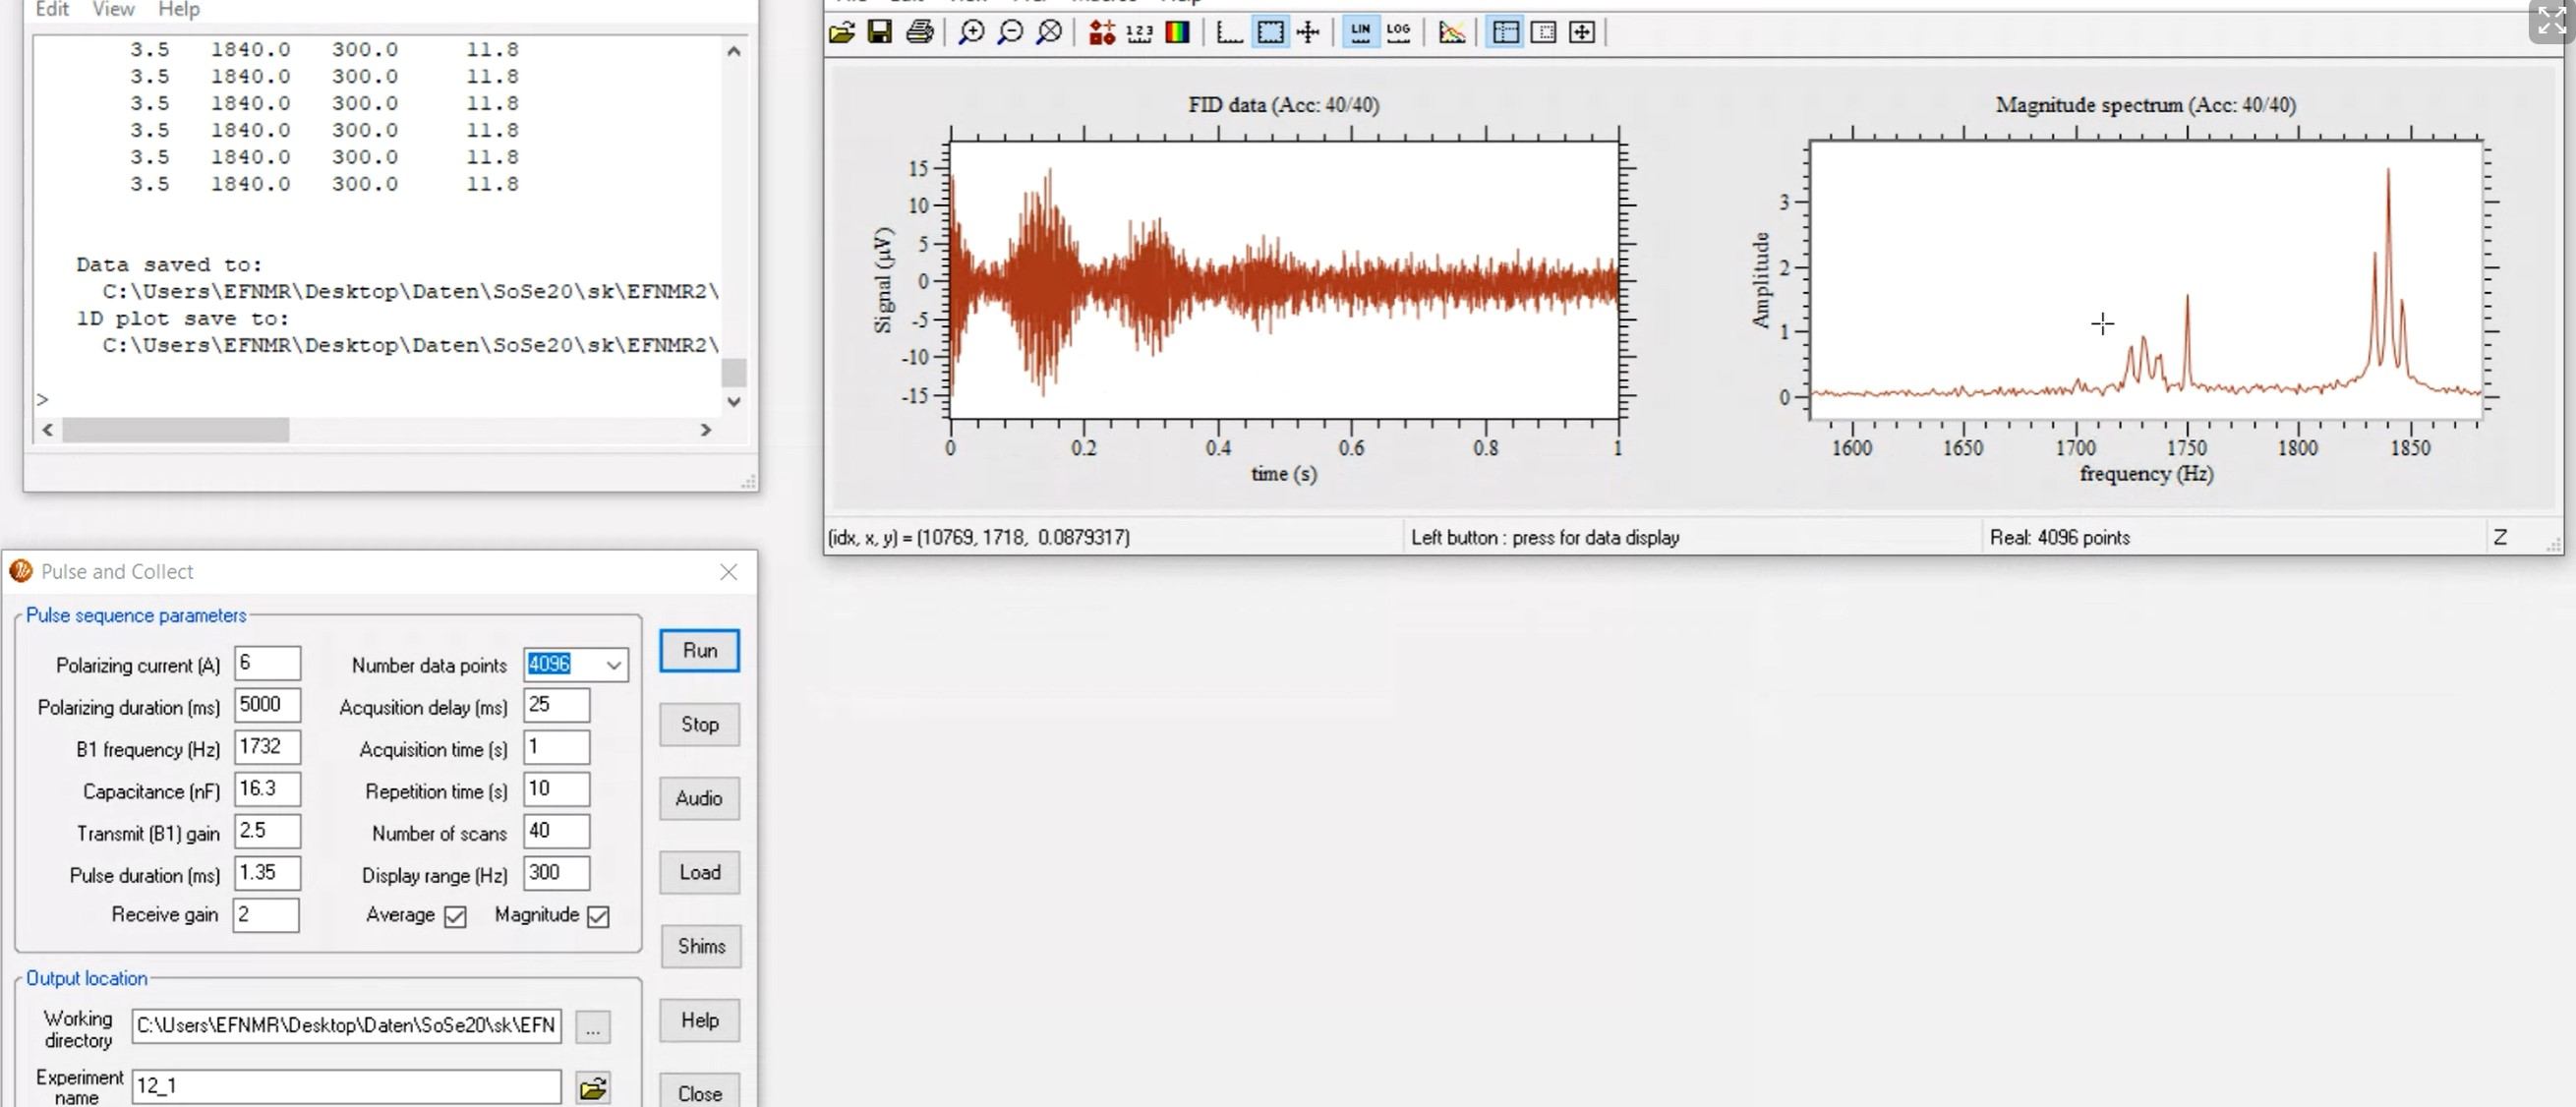
\includegraphics[width=0.8\textwidth]{Screenshot2/12_1.jpg}
        \caption{12.1}
    \end{figure}


\begin{tabular}{ll}

    \textbf{Werte}&            \\
    
       1732.24 & Lamorfrequenz für Fluor (Hz) \\
    
       1841.40 & Lamorfrequenz für Wasserstoff (Hz) \\
    
          20.2 & Kapazität getuned für Fluor (theoretisch) (nF) \\
    
          15.6 & Kapazität getuned für Fluor (empirisch)(Kapazität Wasserstoff 13.8nF) (nF) \\
    
          13.8 & Kapazität getuned für Wasserstoff (empirisch) (nF) \\
    
          17.9 & Kapazität getuned für Wasserstoff (theoretisch) (nF) \\
    
       1786.82 & Mittelwert Frequenzen \\
    
         19.05 & Kapazität Mittelwert (theoretisch) \\
    
          14.7 & Kapazität Mittelwert (empirisch) \\
    
    \end{tabular}  


    \vspace{1cm}




\begin{tabular}{ll}

    \textbf{Durchführung} & \\

    12.1 & Tunen Werte auf Mittelwerte von H und F \\

    12.2 & Run Pulse and collect experiment \\

    12.3 & Tune auf gute Werte der Frequenzen und run pulse and collect\\

\end{tabular}  

\subsection{2D Messung (1.5h)}


% Table generated by Excel2LaTeX from sheet 'Sheet1'
\begin{tabular}{ll}
    \textbf{Durchführung} & \\

    14.1 & T1:  Open ''GradientEchoImaging'': 2D mode; ''YZ'' Orientation; \\

         &  FOV: 120mm; matrix: 32*16 (zero-filled to 64*64);  \\

         & B1 frequency: 1837 Hz, phase gradient duration: 50ms; echo time: 200ms;  \\

         &  bandwidth: 64Hz; number of scans: 4 with filtering; \\

    14.2 & (TR: 50\%! Ca. 4s) polarisation time gleich wie kleinste gemessene T1 \textbf{Startwert $T_1 \approx 600$ms}\\

    14.3 & (TR: 50\%!) polarisation time Mittelwert aus T1´s \\

    14.4 & (TR: 50\%! Ca 8 s) polarisation time gleich wie größte gemessene T1\\

    14.5 & (TR: 50\%!) polarisation time doppelt so lange wie größte T1\\

    15.1 & T2:  Open ''GradientEchoImaging'': 2D mode; ''YZ'' Orientation; \\

         &  FOV: 120mm; matrix: 32*16 
         \textbf{32*32 gesetzt als erstes, anschließend runtergesetzt auf wieder 16*16; Number of scans von 3 auf 1 $\rightarrow$ Unsicherheit größer)} (zero-filled to 64*64);  \\

         & B1 frequency: 1837 Hz, phase gradient duration: 50ms; echo time: 200ms;  \\

         &  bandwidth: 64Hz; number of scans: 4 with filtering; \\

         & polarizing duration aus Schritt 14.5 \\

    15.2 & kürzest mögliche echo time (ca. 200ms) \\

    15.3 & echo time (ca. 250 ms) \\

    15.4 & echo time (ca. 300ms) \\

    15.5 & echo time (ca. 450ms) \\

    15.6 & echo time (ca. 550)\\
\end{tabular}  



\begin{figure}[H]
    \centering
    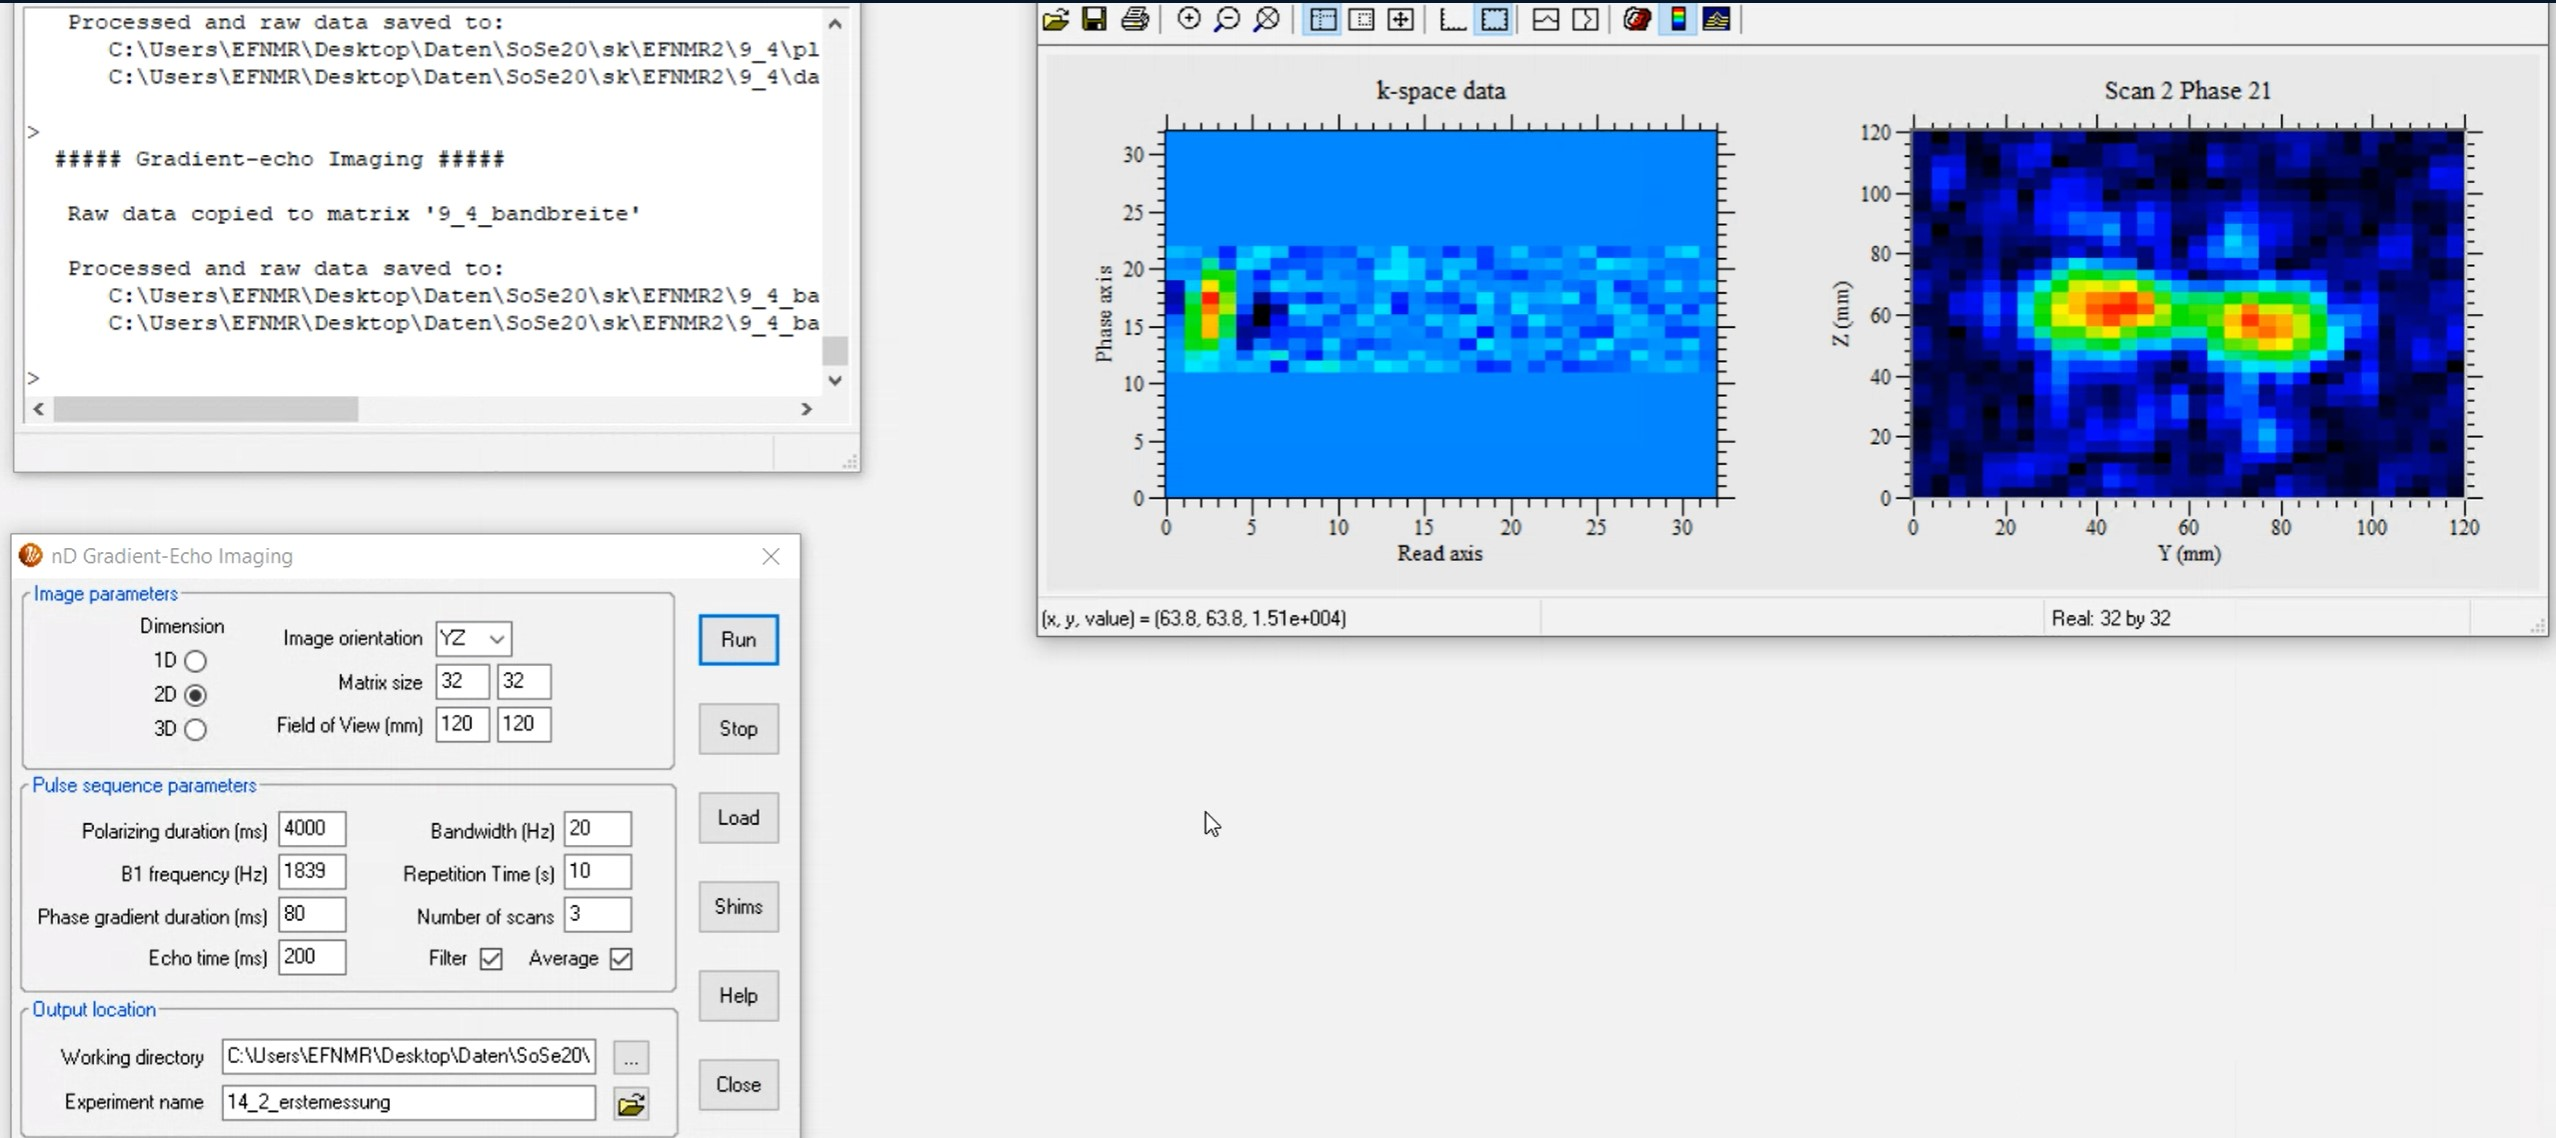
\includegraphics[width = 0.8\textwidth]{Screenshot2/14_2ersteMessung.jpg}
\end{figure}

\begin{figure}[H]
    \centering
    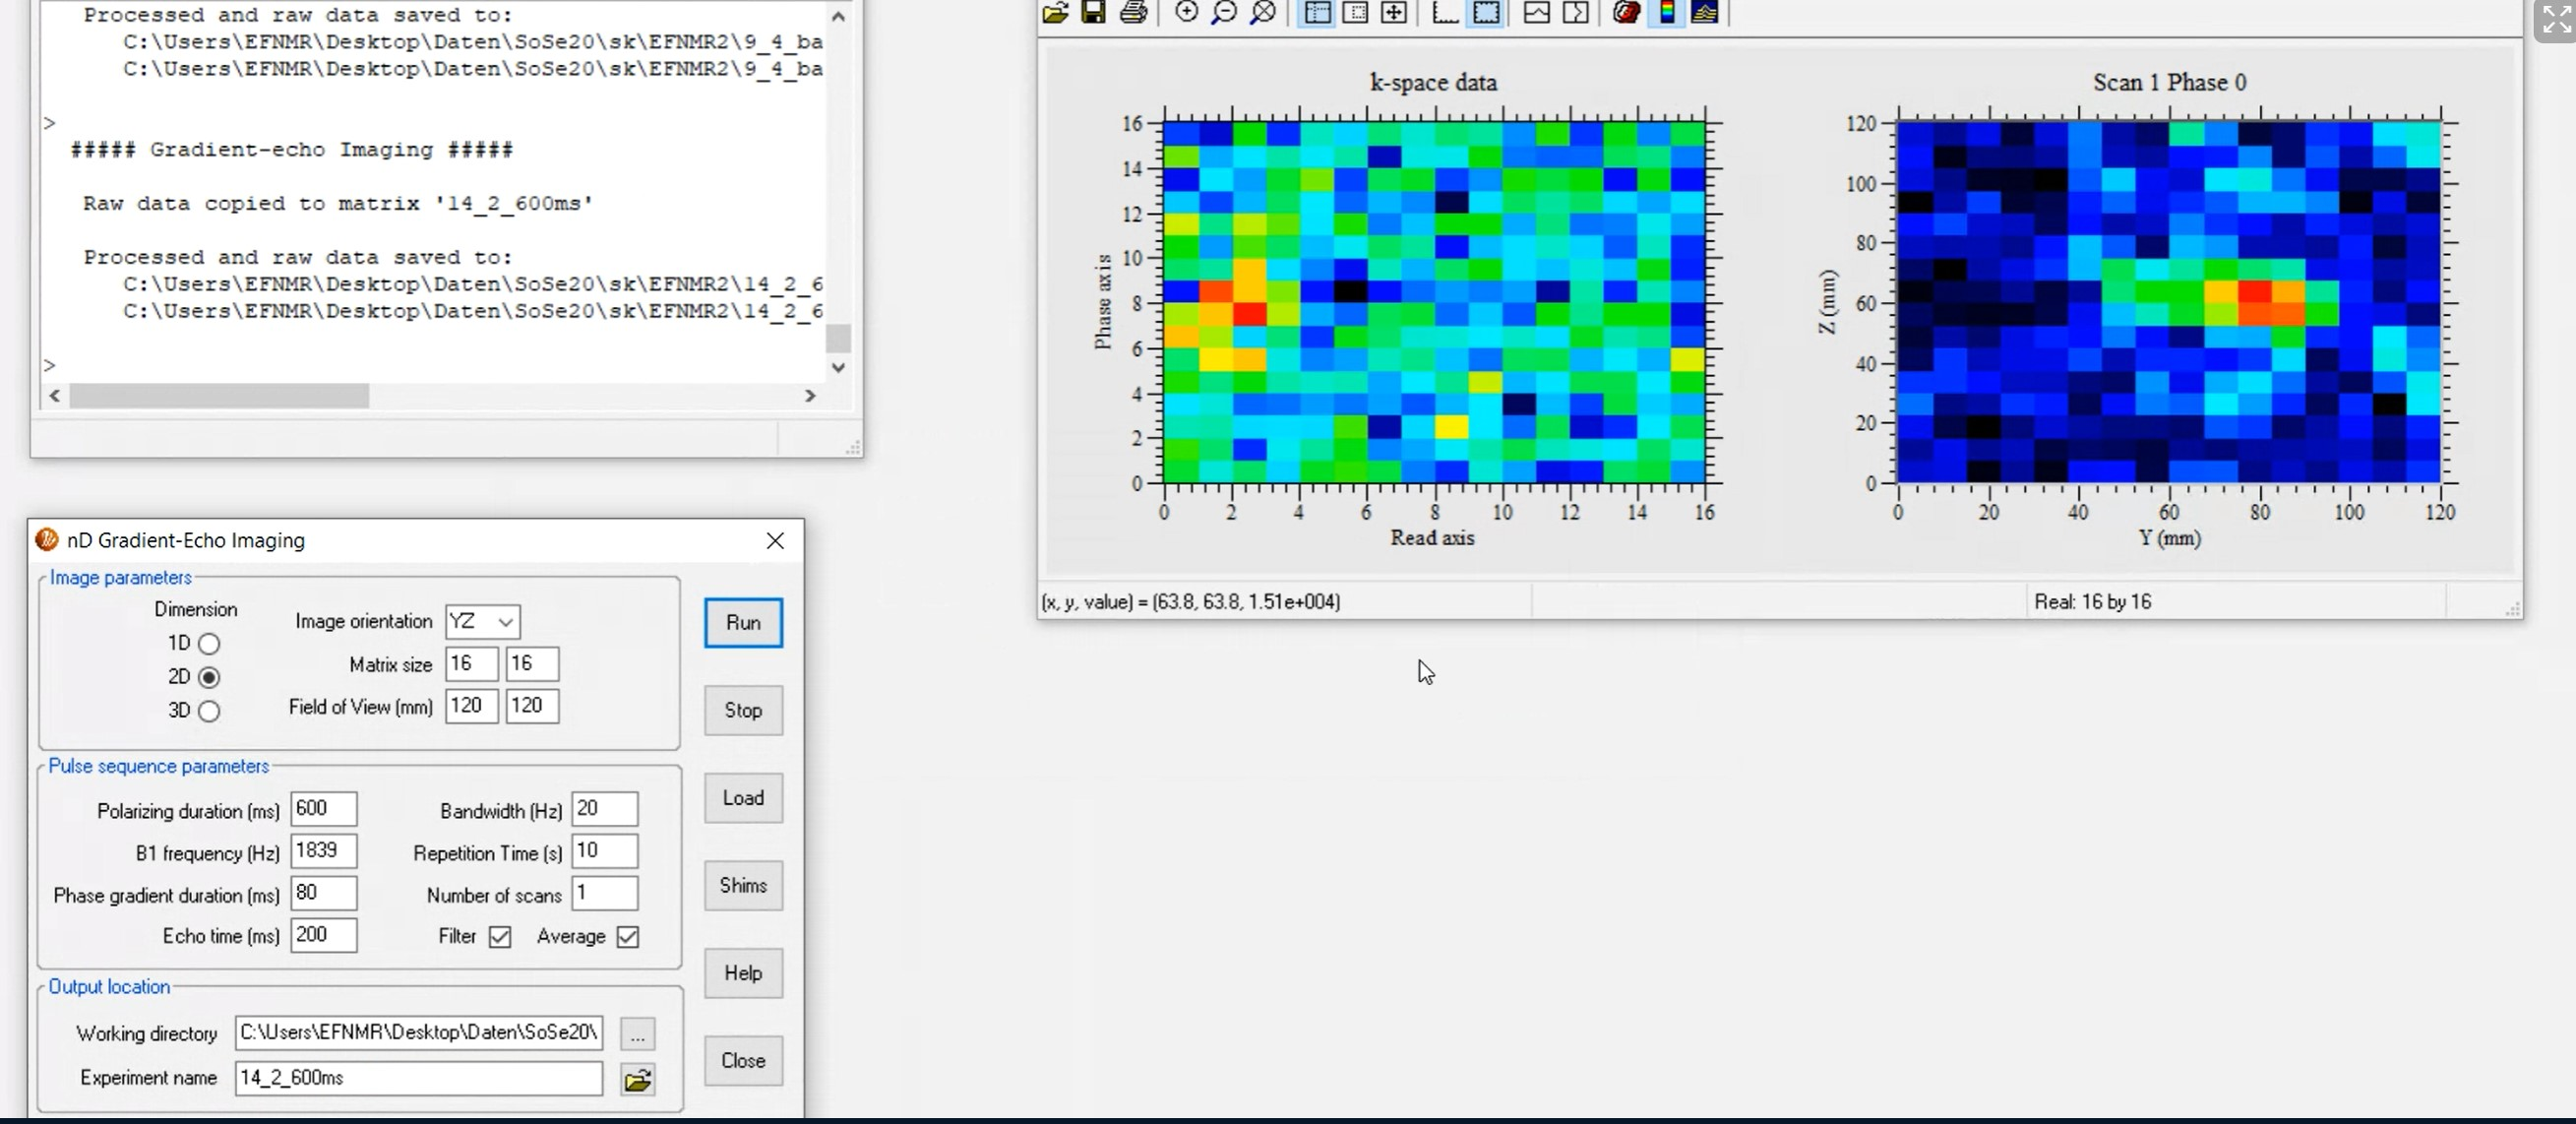
\includegraphics[width = 0.8\textwidth]{Screenshot2/14_2_600ms.jpg}
\end{figure}

\begin{figure}[H]
    \centering
    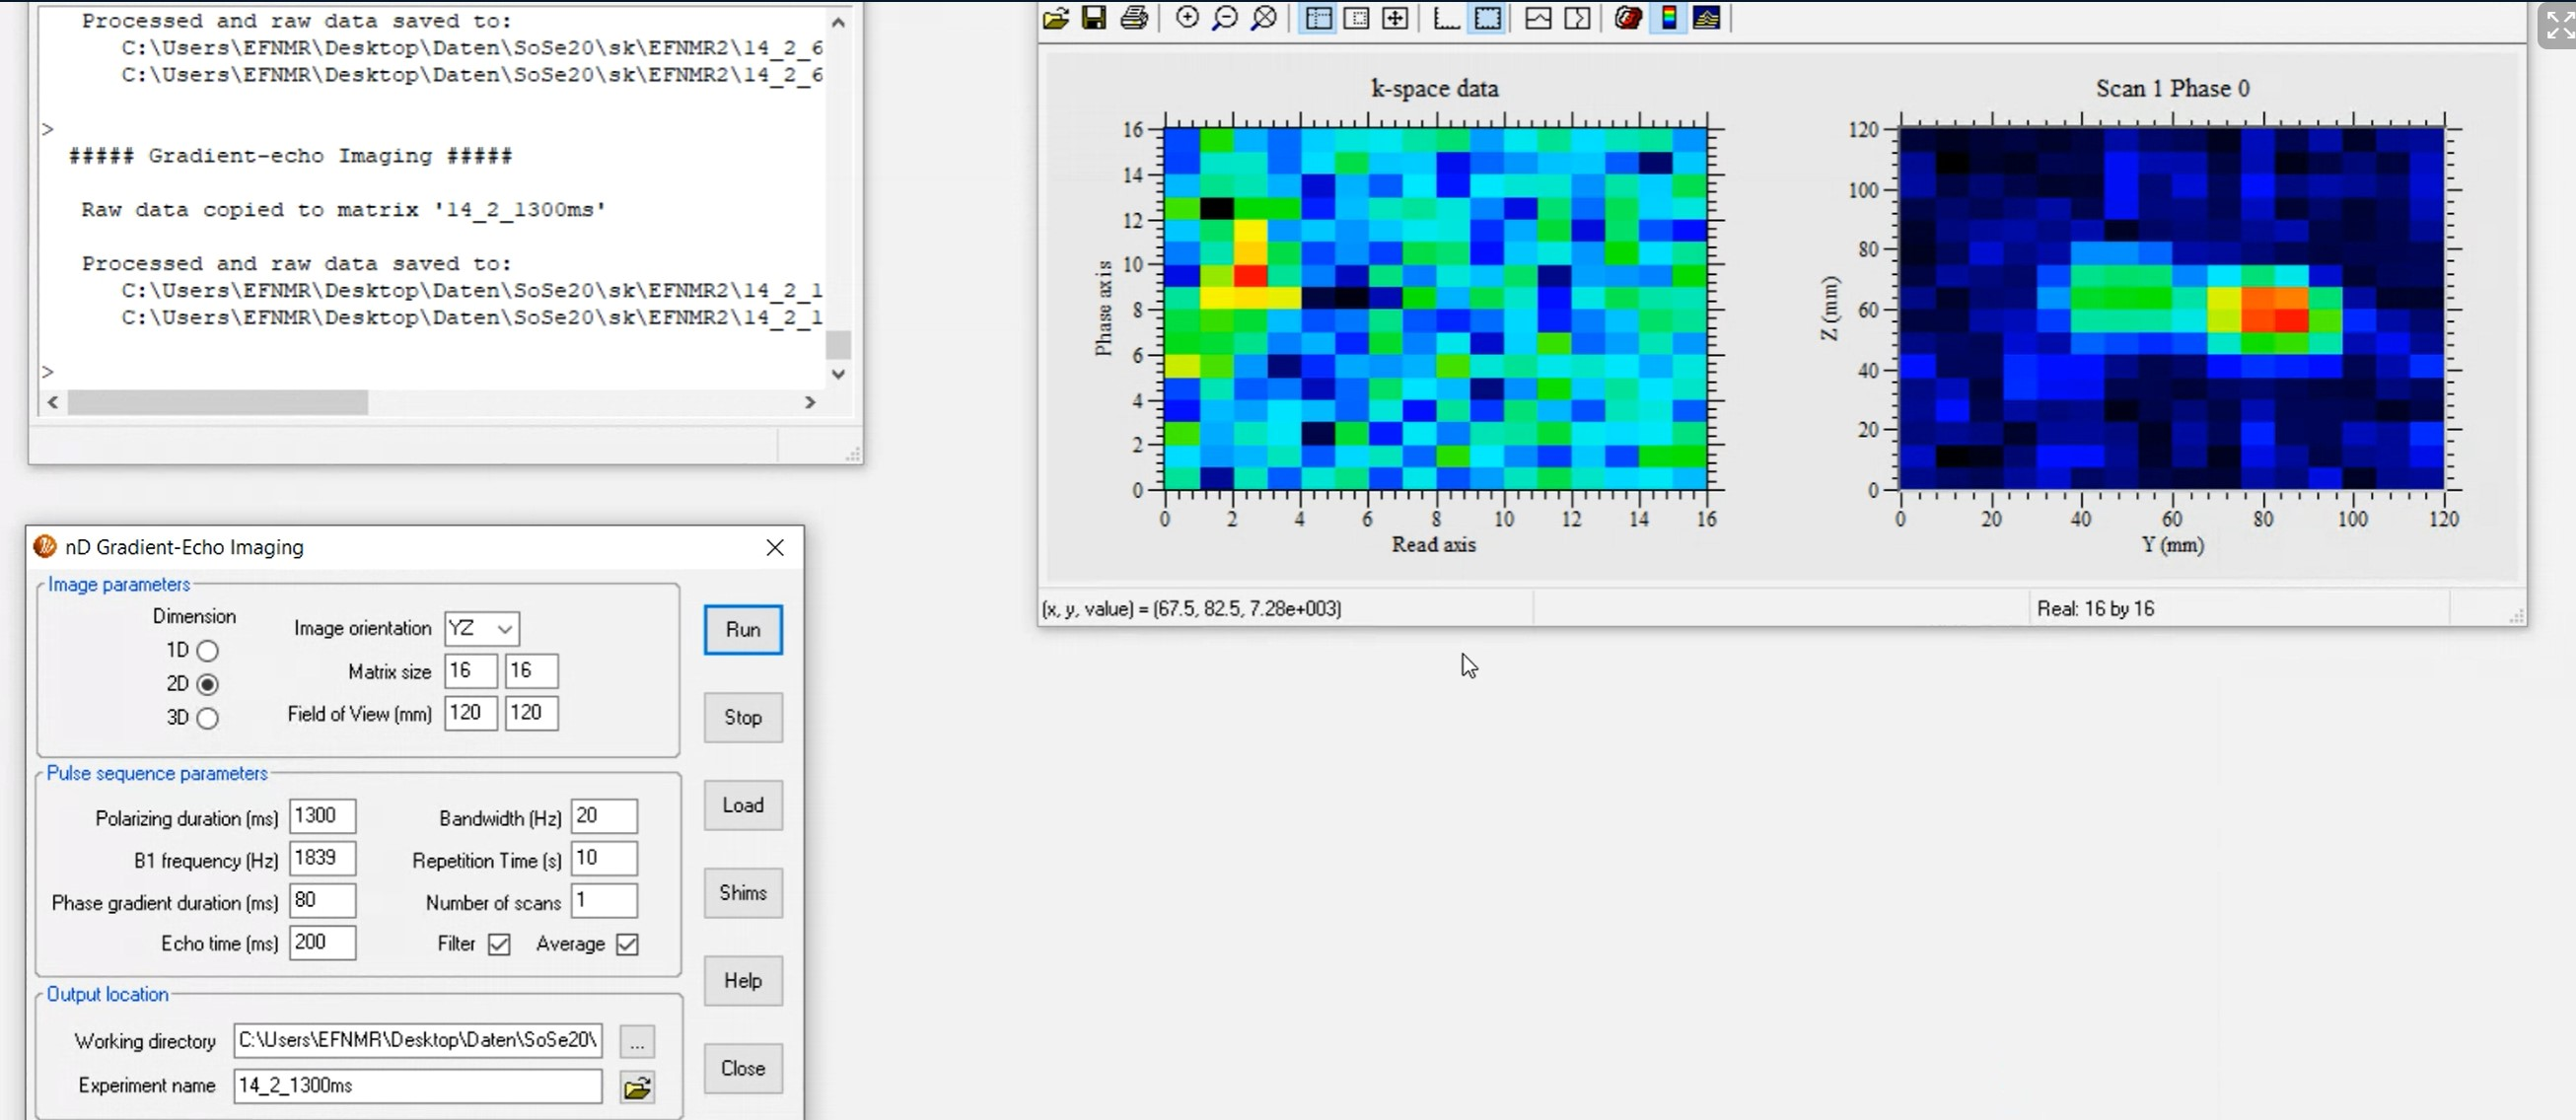
\includegraphics[width = 0.8\textwidth]{Screenshot2/14_2_1300ms.jpg}
\end{figure}


\begin{figure}[H]
    \centering
    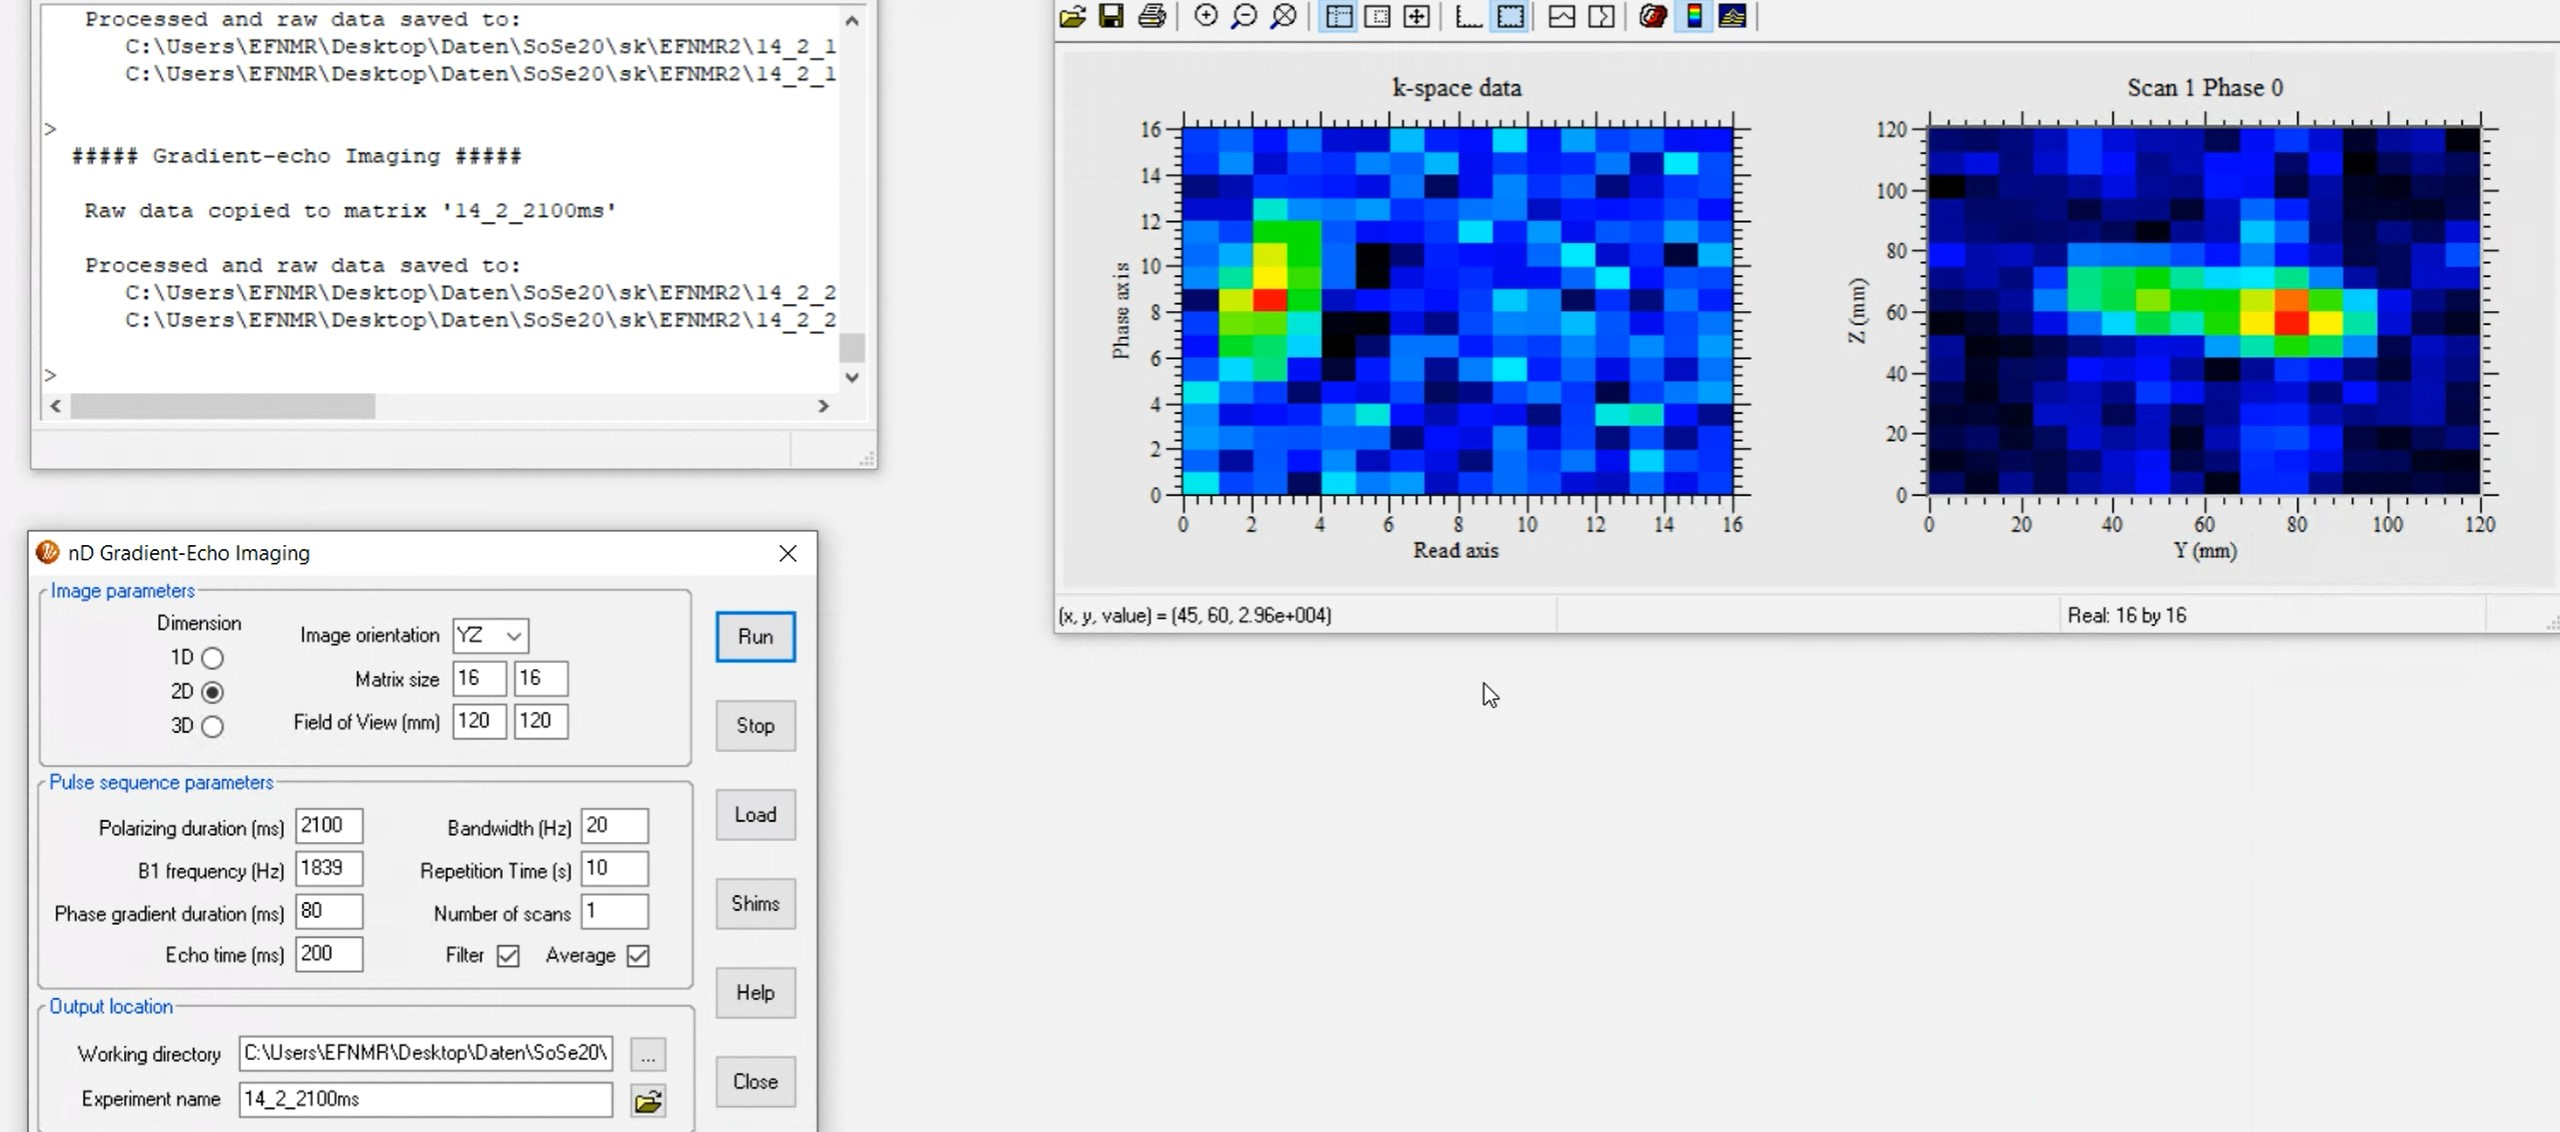
\includegraphics[width = 0.8\textwidth]{Screenshot2/14_2_2100ms.jpg}
\end{figure}


\begin{figure}[H]
    \centering
    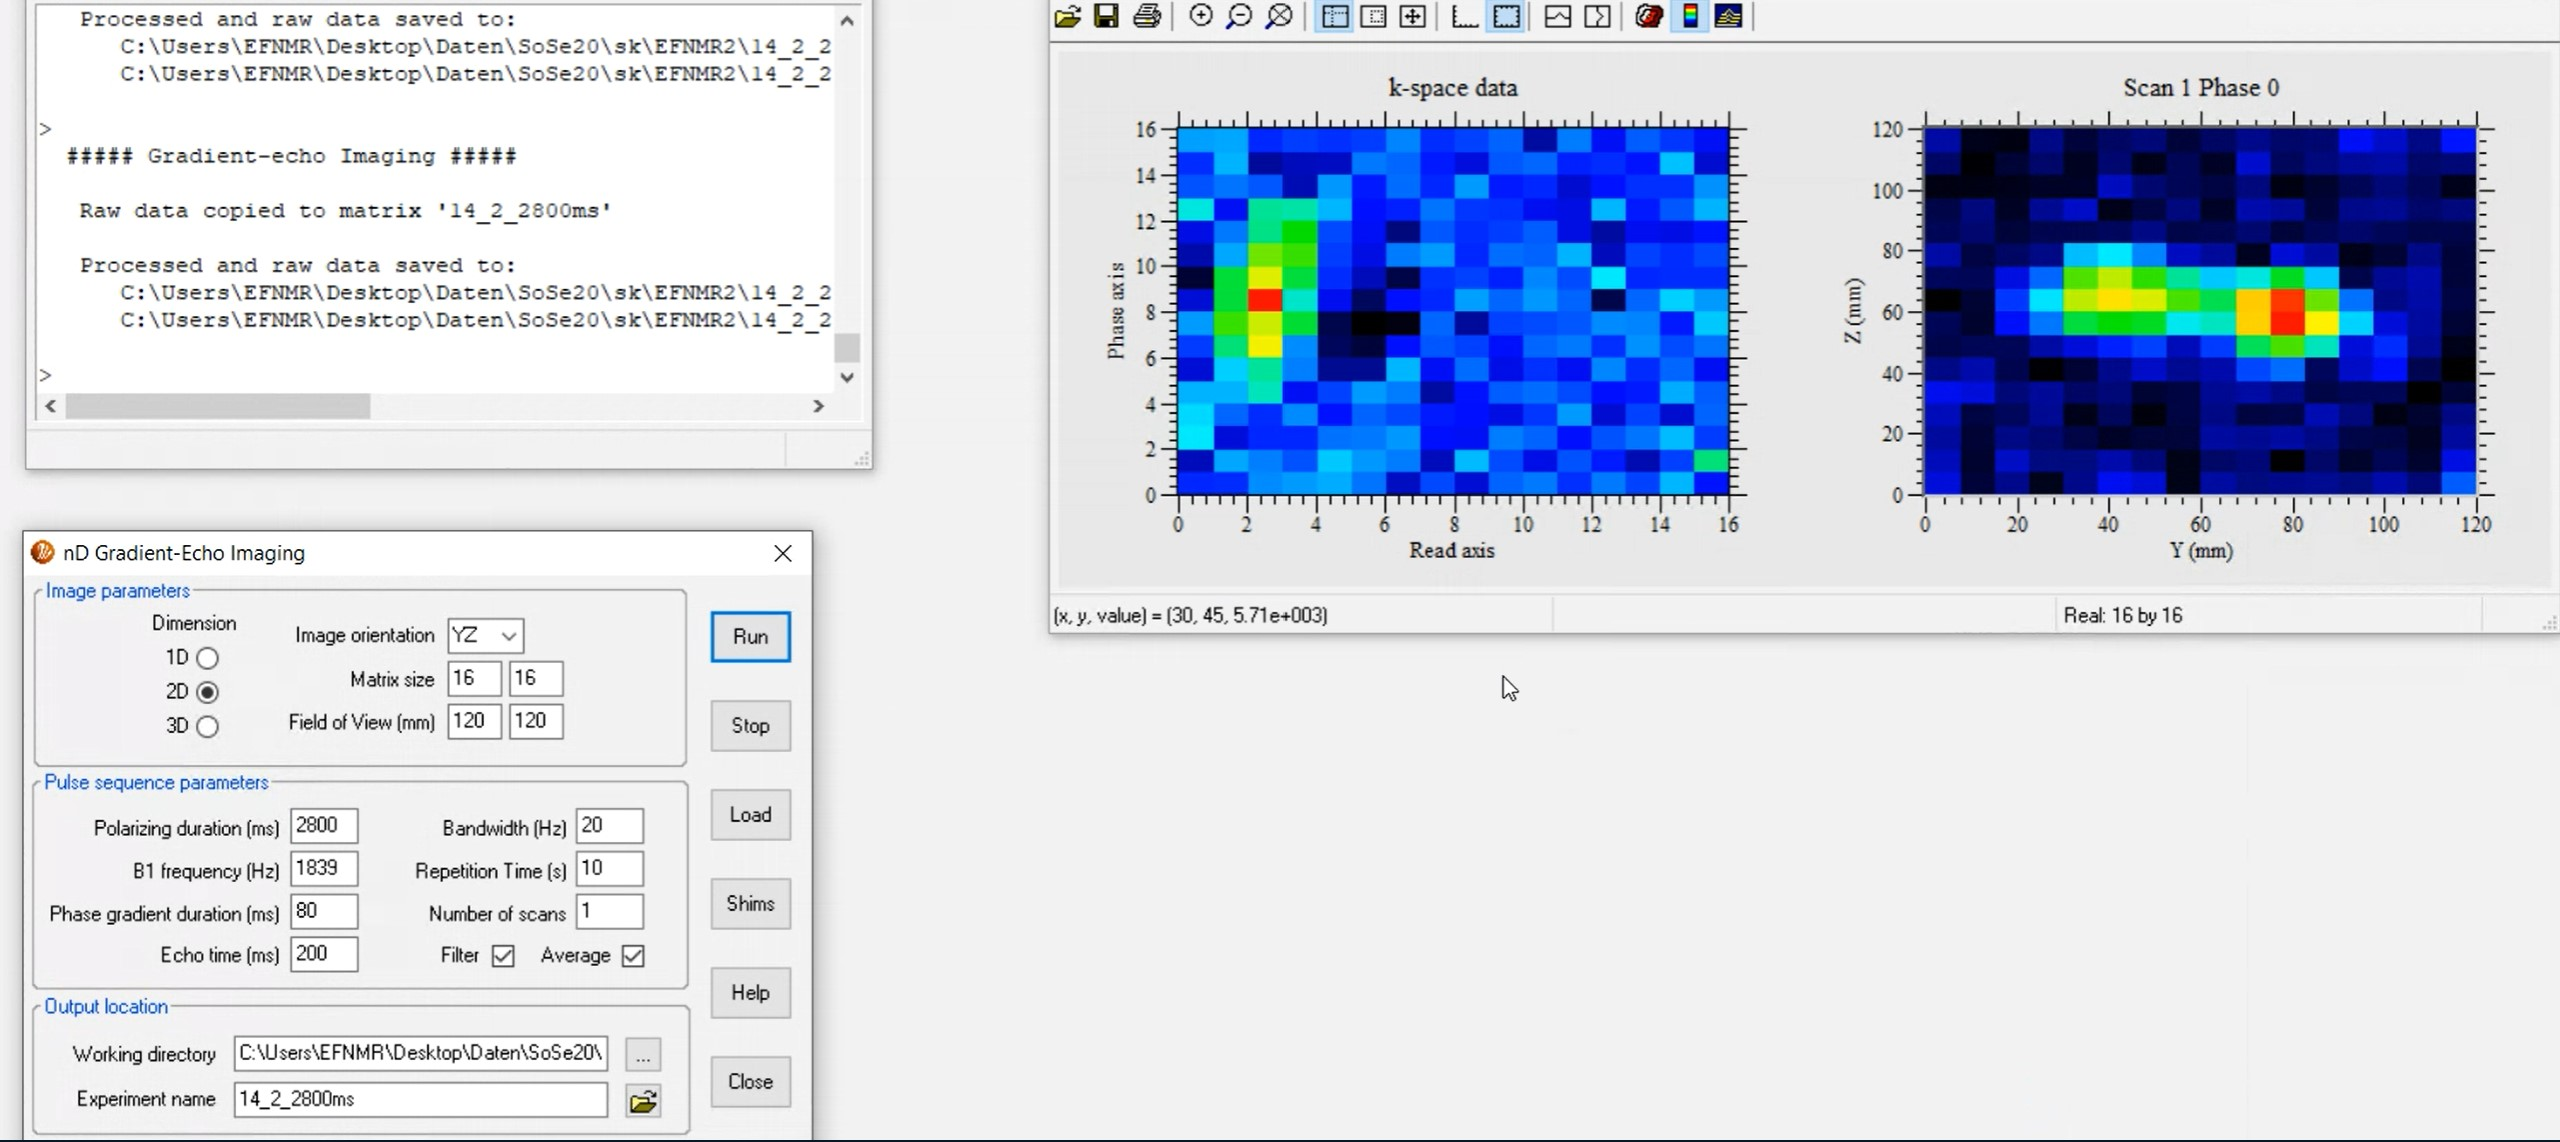
\includegraphics[width = 0.8\textwidth]{Screenshot2/14_2_2800ms.jpg}
\end{figure}

\textbf{15.2 ab hier}
\begin{figure}[H]
    \centering
    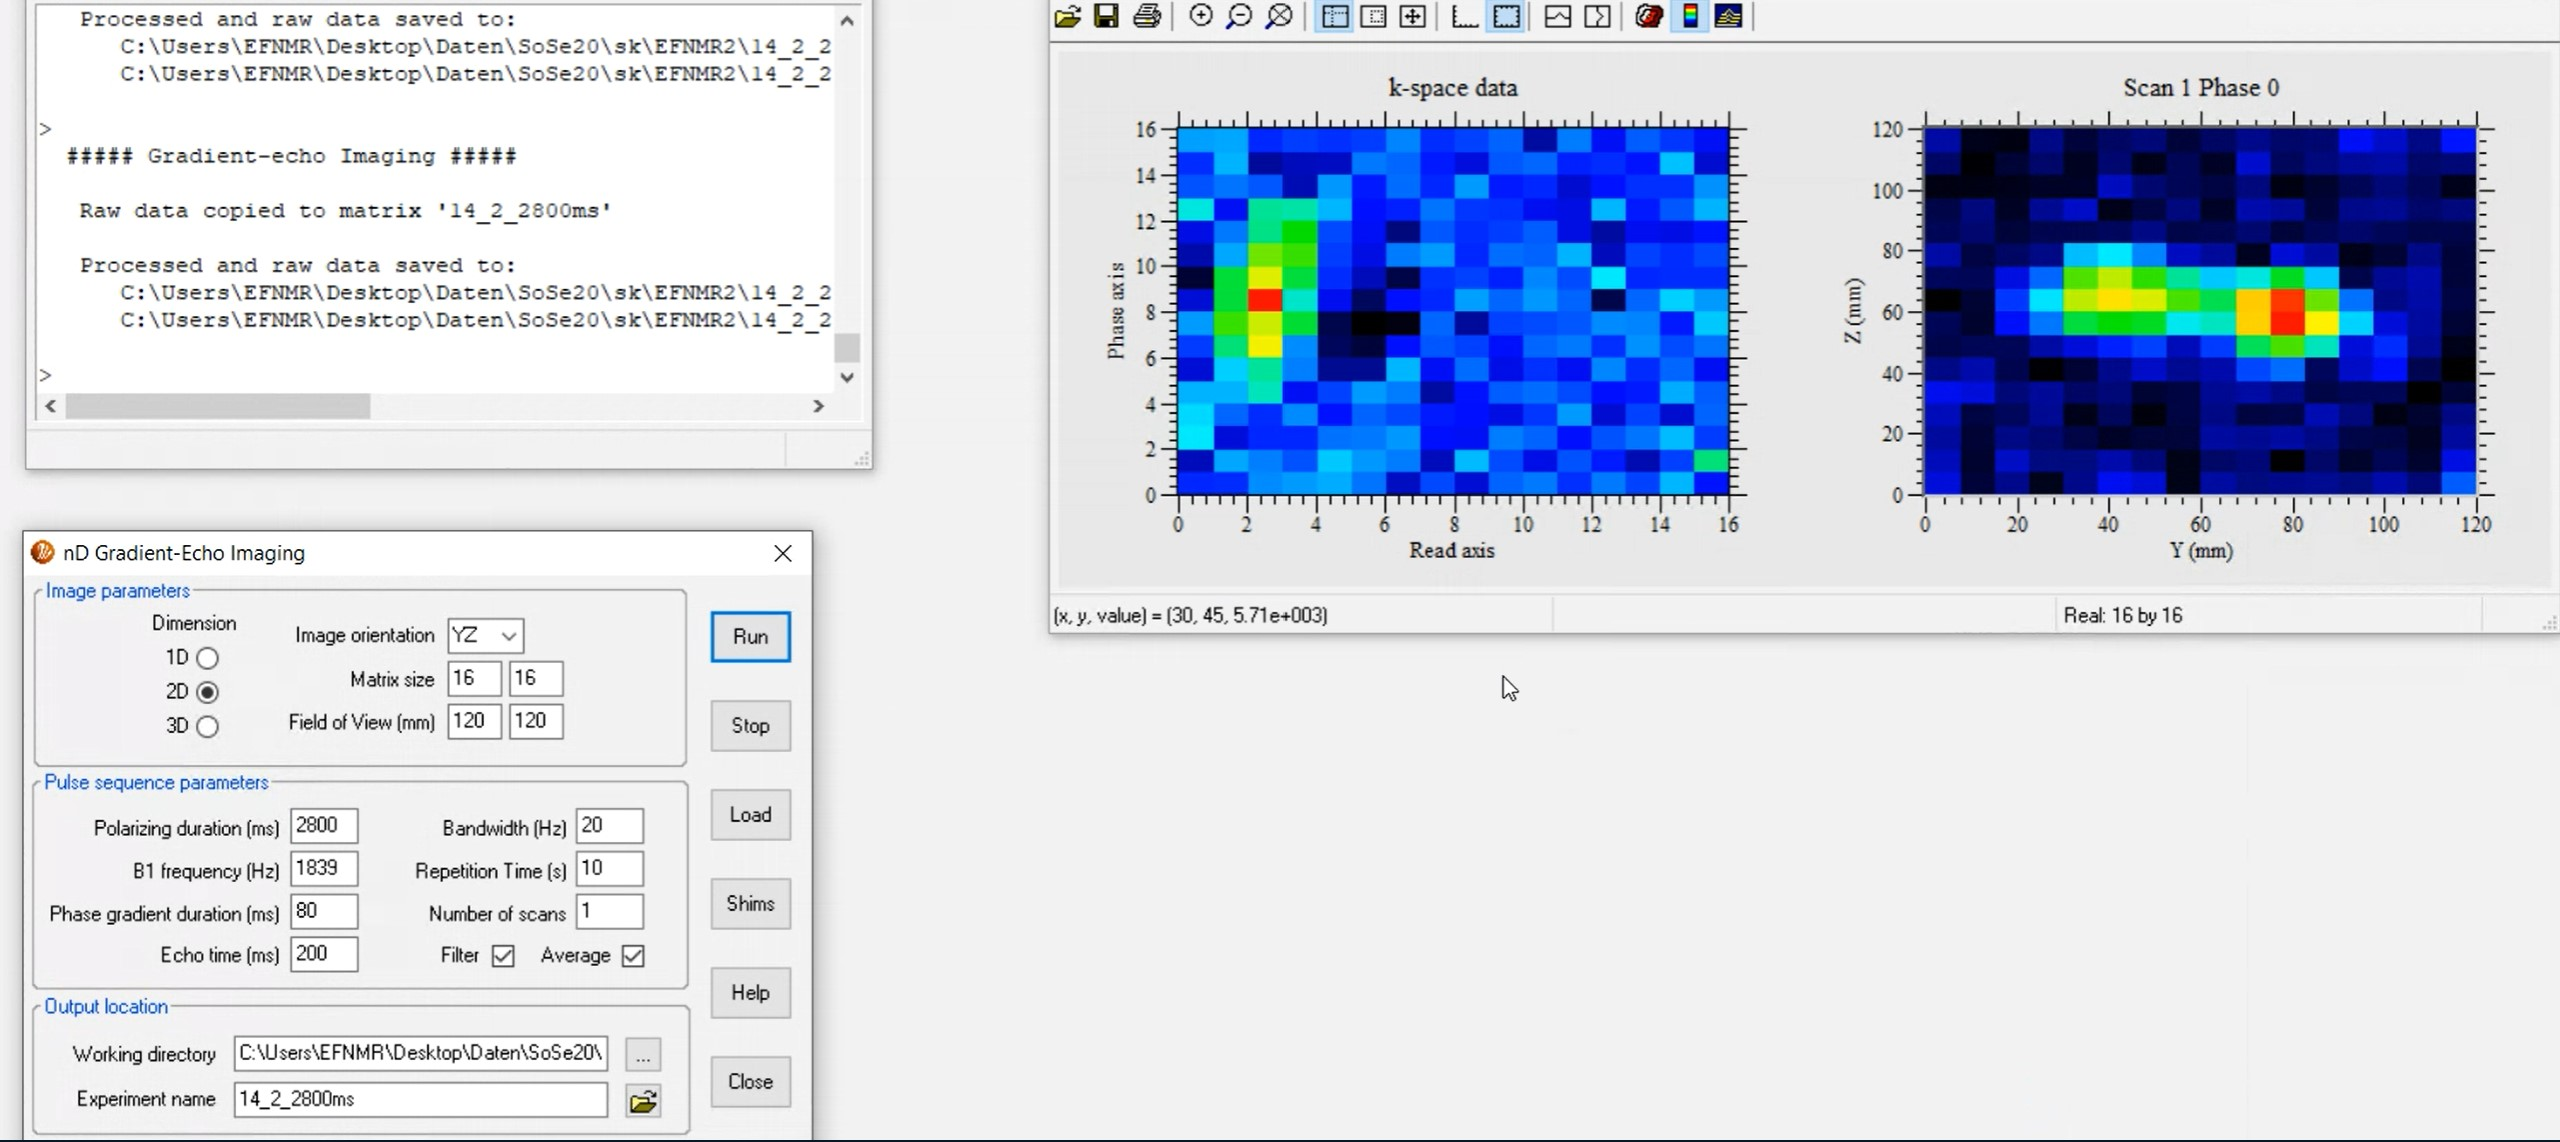
\includegraphics[width = 0.8\textwidth]{Screenshot2/14_2_2800ms.jpg}
\end{figure}

\begin{figure}[H]
    \centering
    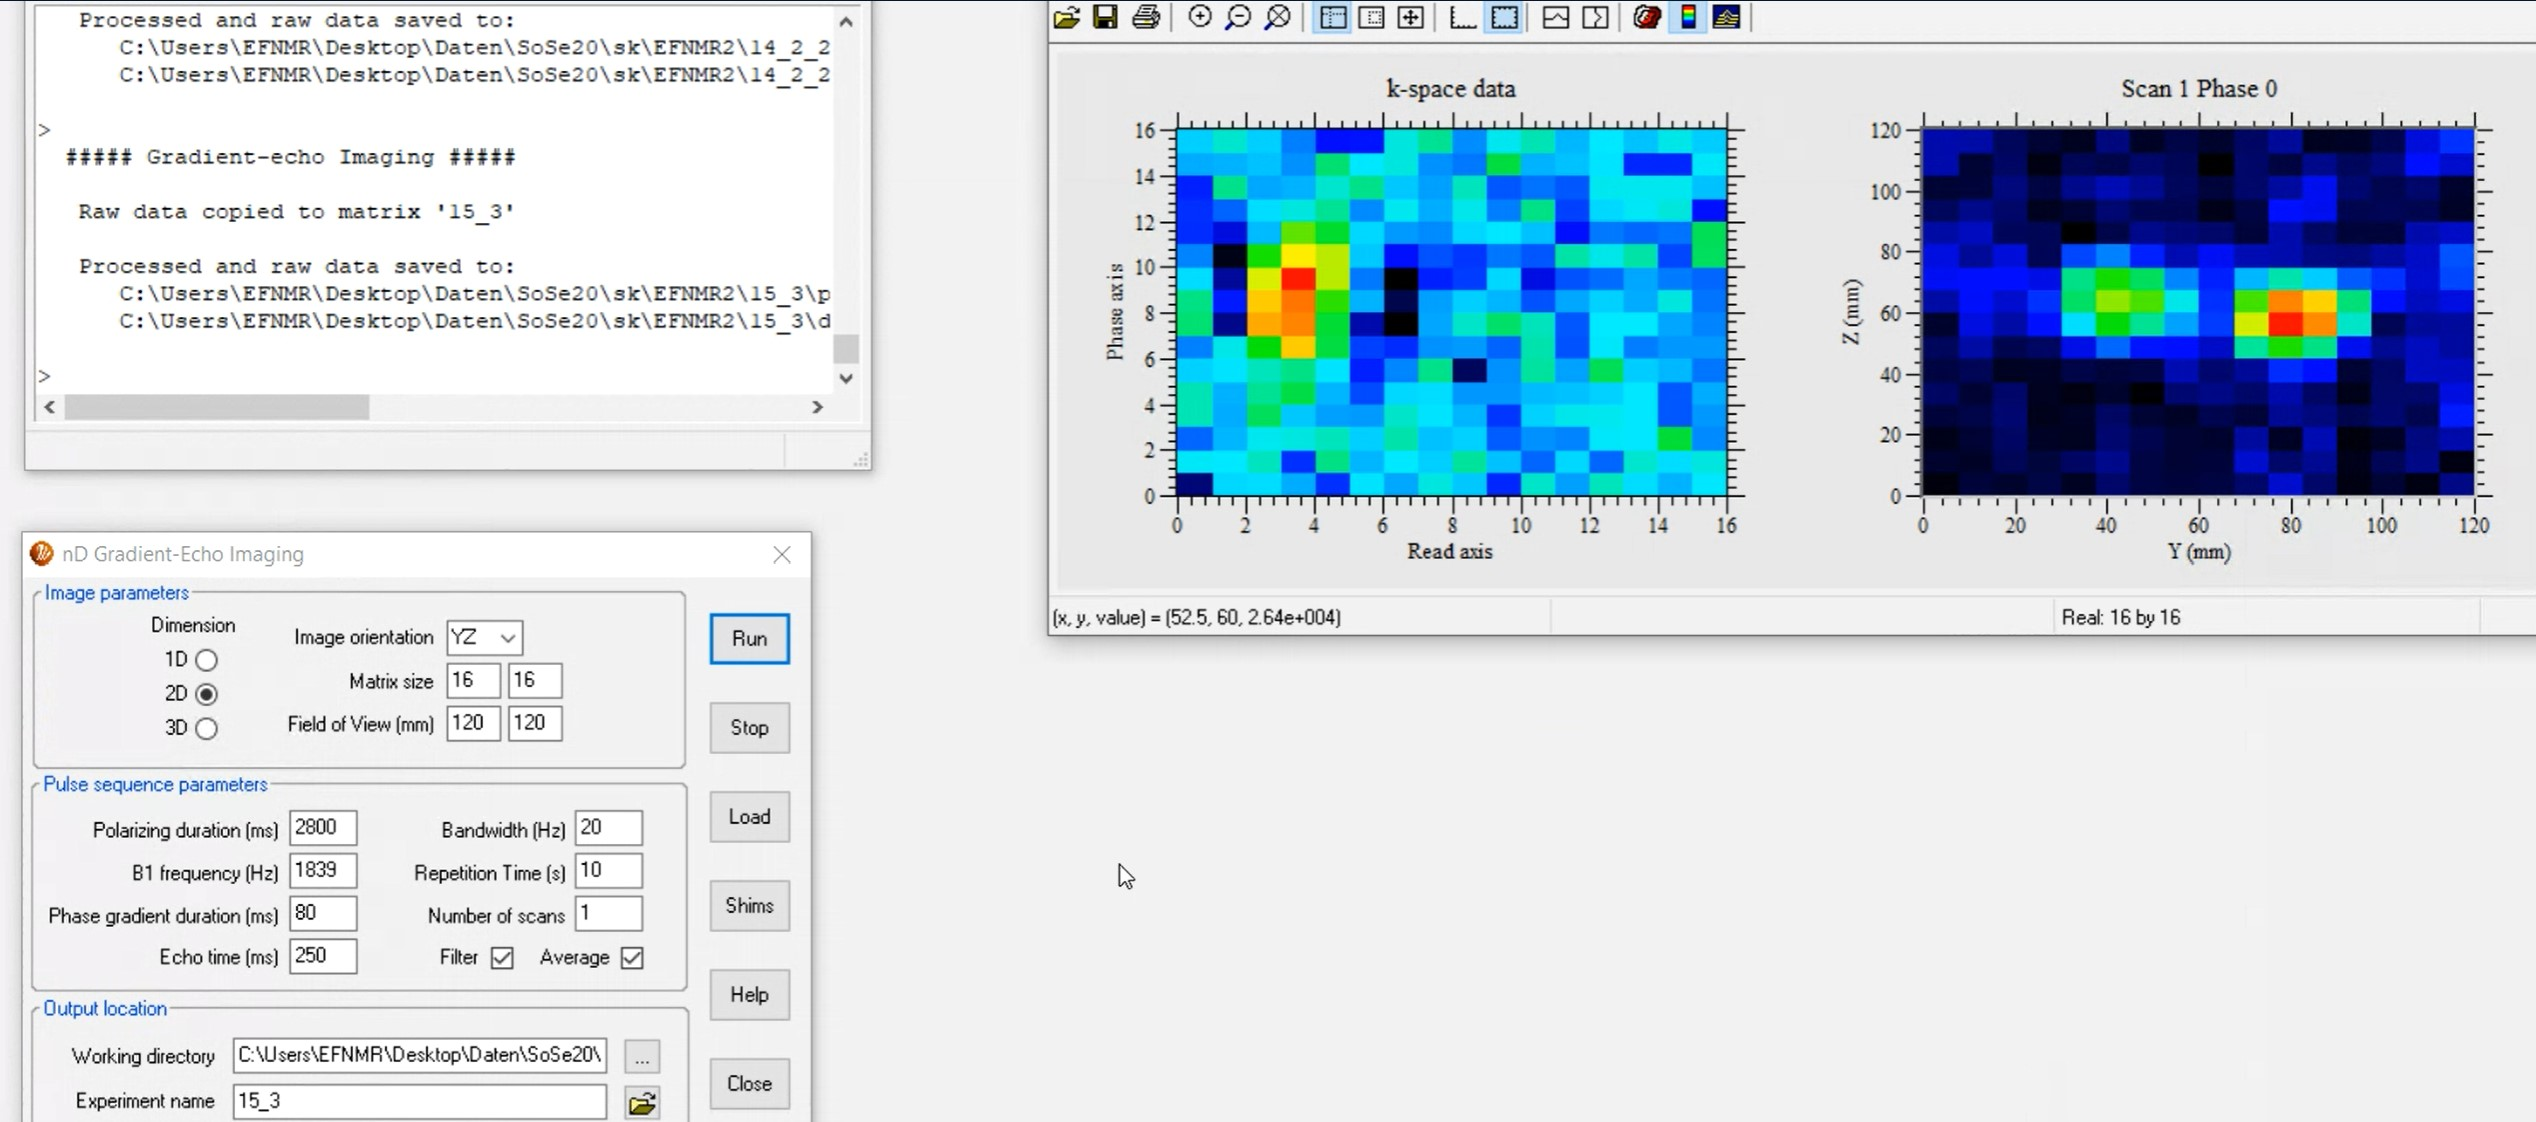
\includegraphics[width = 0.8\textwidth]{Screenshot2/15_3.jpg}
\end{figure}

\begin{figure}[H]
    \centering
    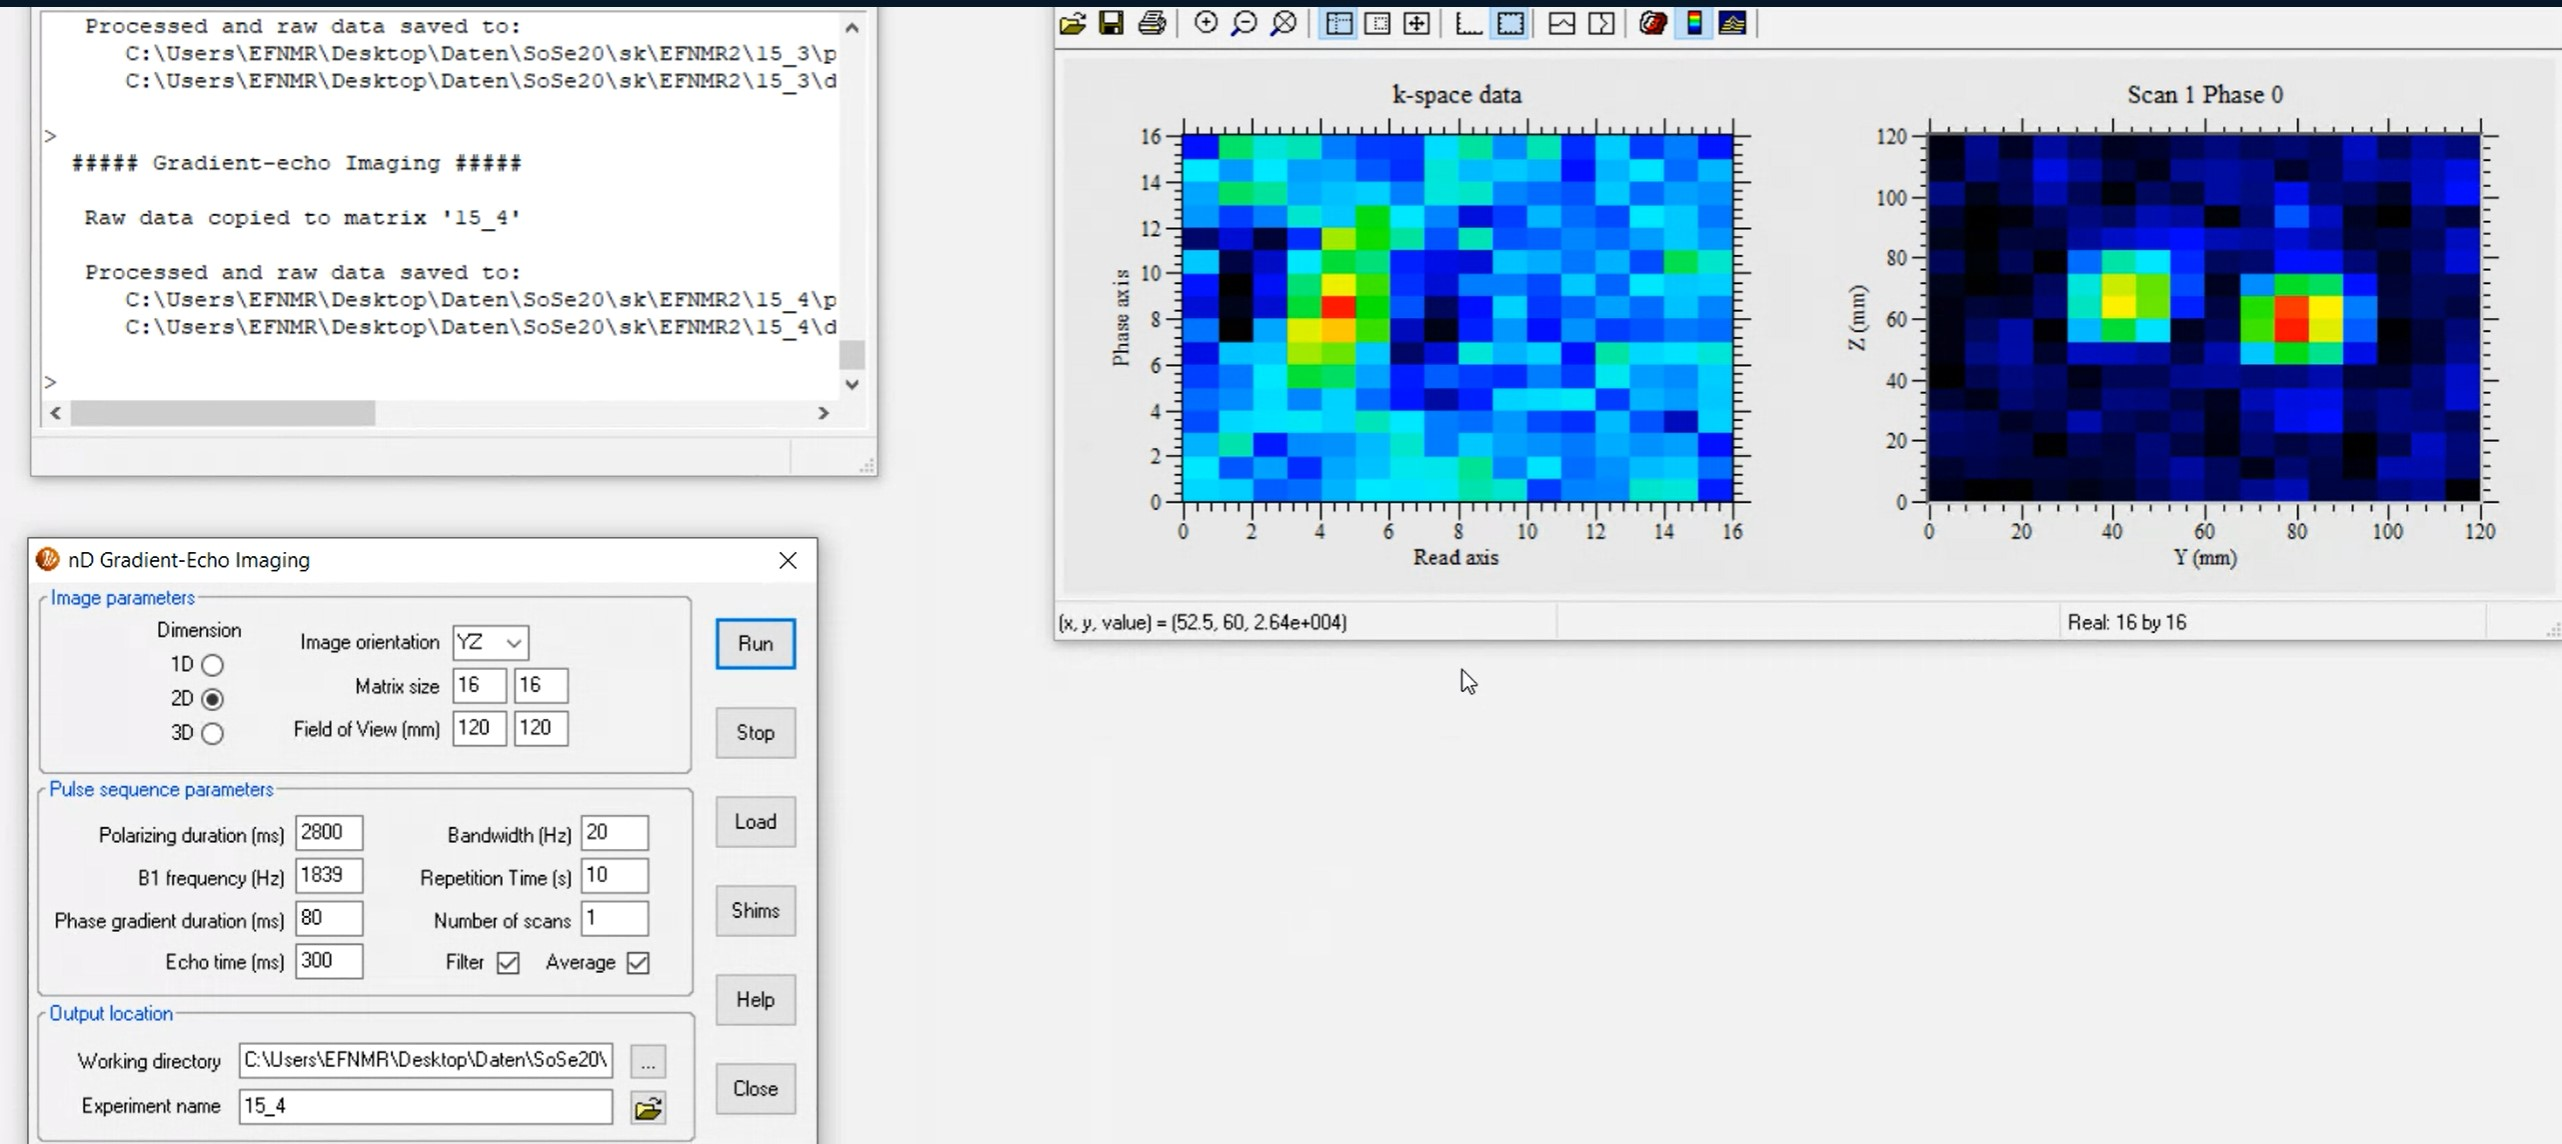
\includegraphics[width = 0.8\textwidth]{Screenshot2/15_4.jpg}
\end{figure}


\begin{figure}[H]
    \centering
    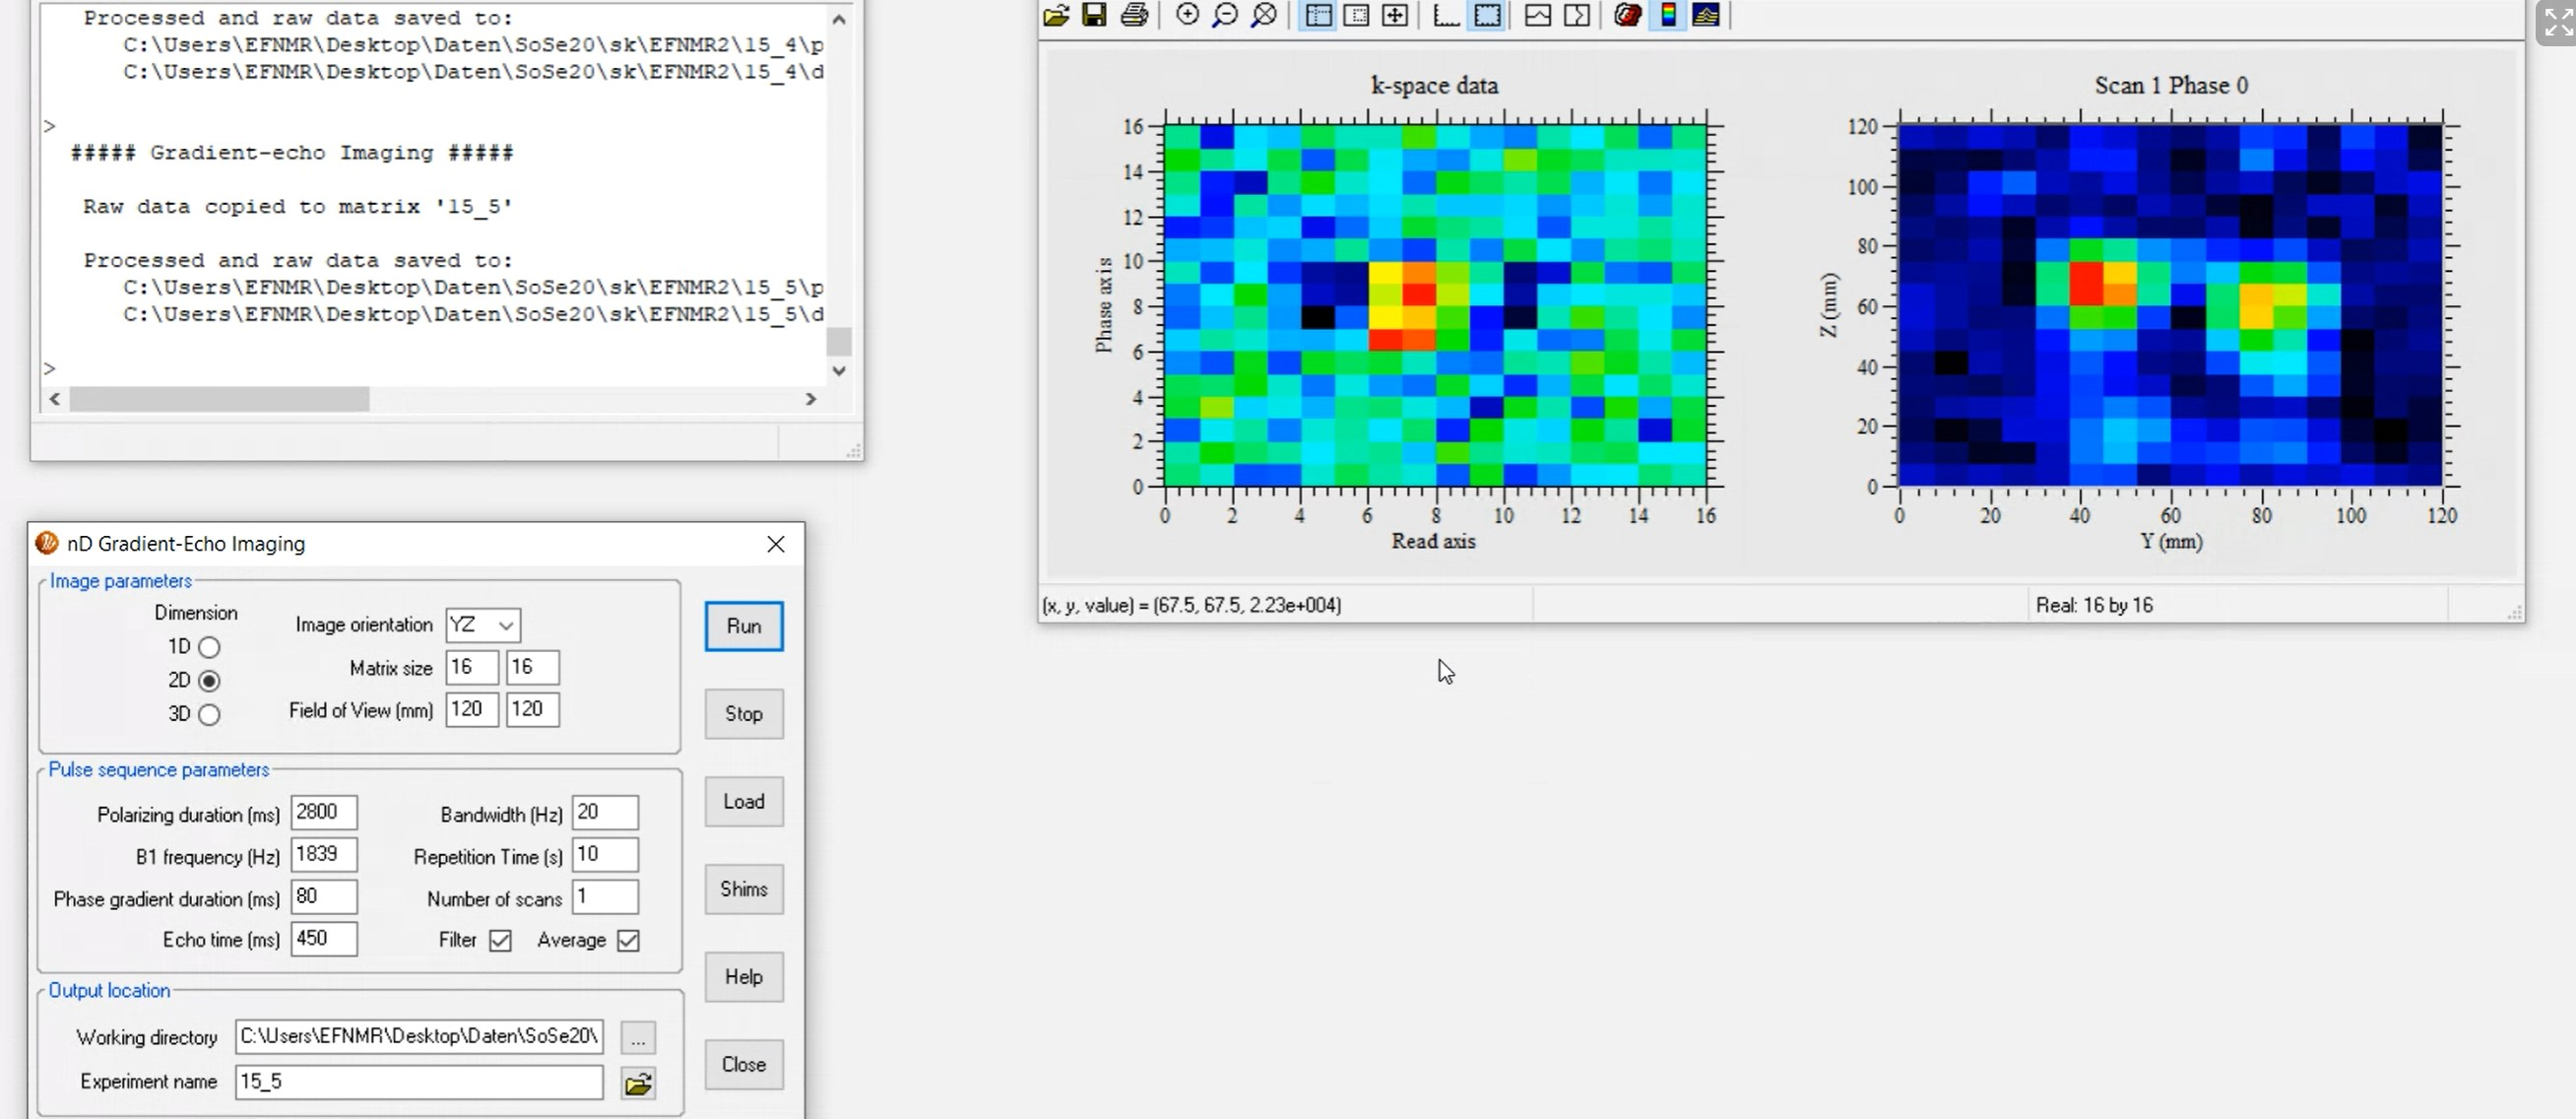
\includegraphics[width = 0.8\textwidth]{Screenshot2/15_5.jpg}
\end{figure}
\textbf{Polarisationduration wurde erhöht, damit diese für Wasser reicht und alles polarisiert ist}
\begin{figure}[H]
    \centering
    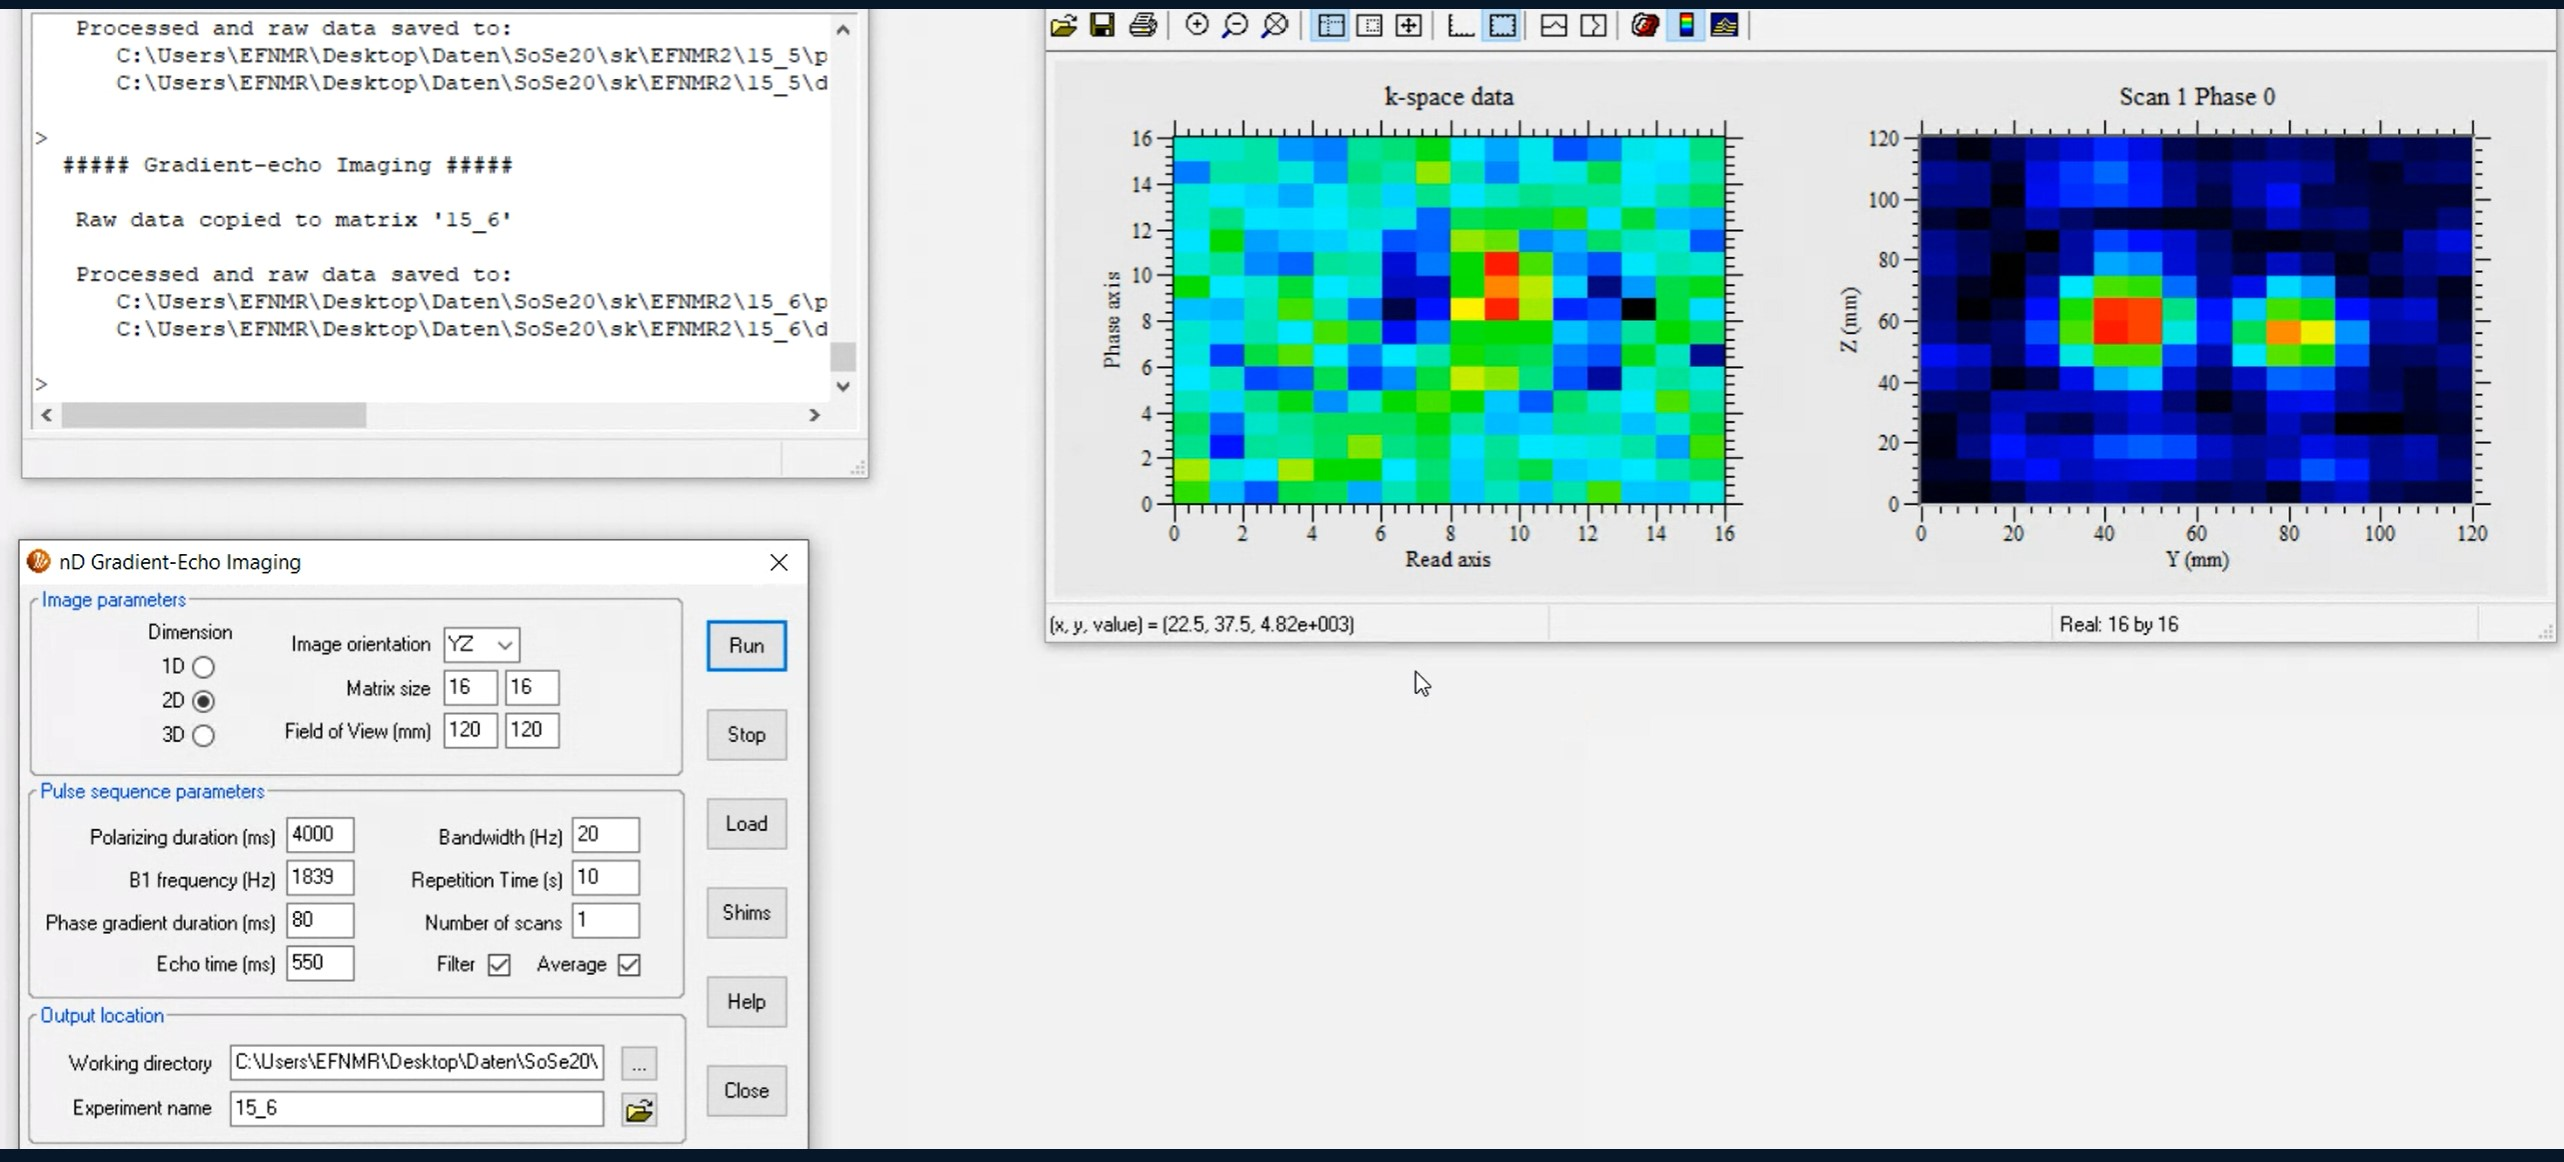
\includegraphics[width = 0.8\textwidth]{Screenshot2/15_6.jpg}
\end{figure}



\subsection{PGSE (0.75h)}


\begin{tabular}{ll}
    \textbf{Durchführung} & \\

    16.1 & Open PGSE dialog \\

    16.2 & Paramter einstellen wie auf Abb. 4.1 + pulse width  \\

         & step size 5 ms und Number of steps 8 siehe Abb. 4.2 \\
\end{tabular} 



Diffusionskoeffizient möglicherweise größer, da es heute wärmer war.\\
Bei der Repetitiontimer hat der PC teilweise einen Fehler ausgeworfen\\
Werte in ln waren negativ und somit Messung früher abgerbochen\\


\begin{figure}[H]
    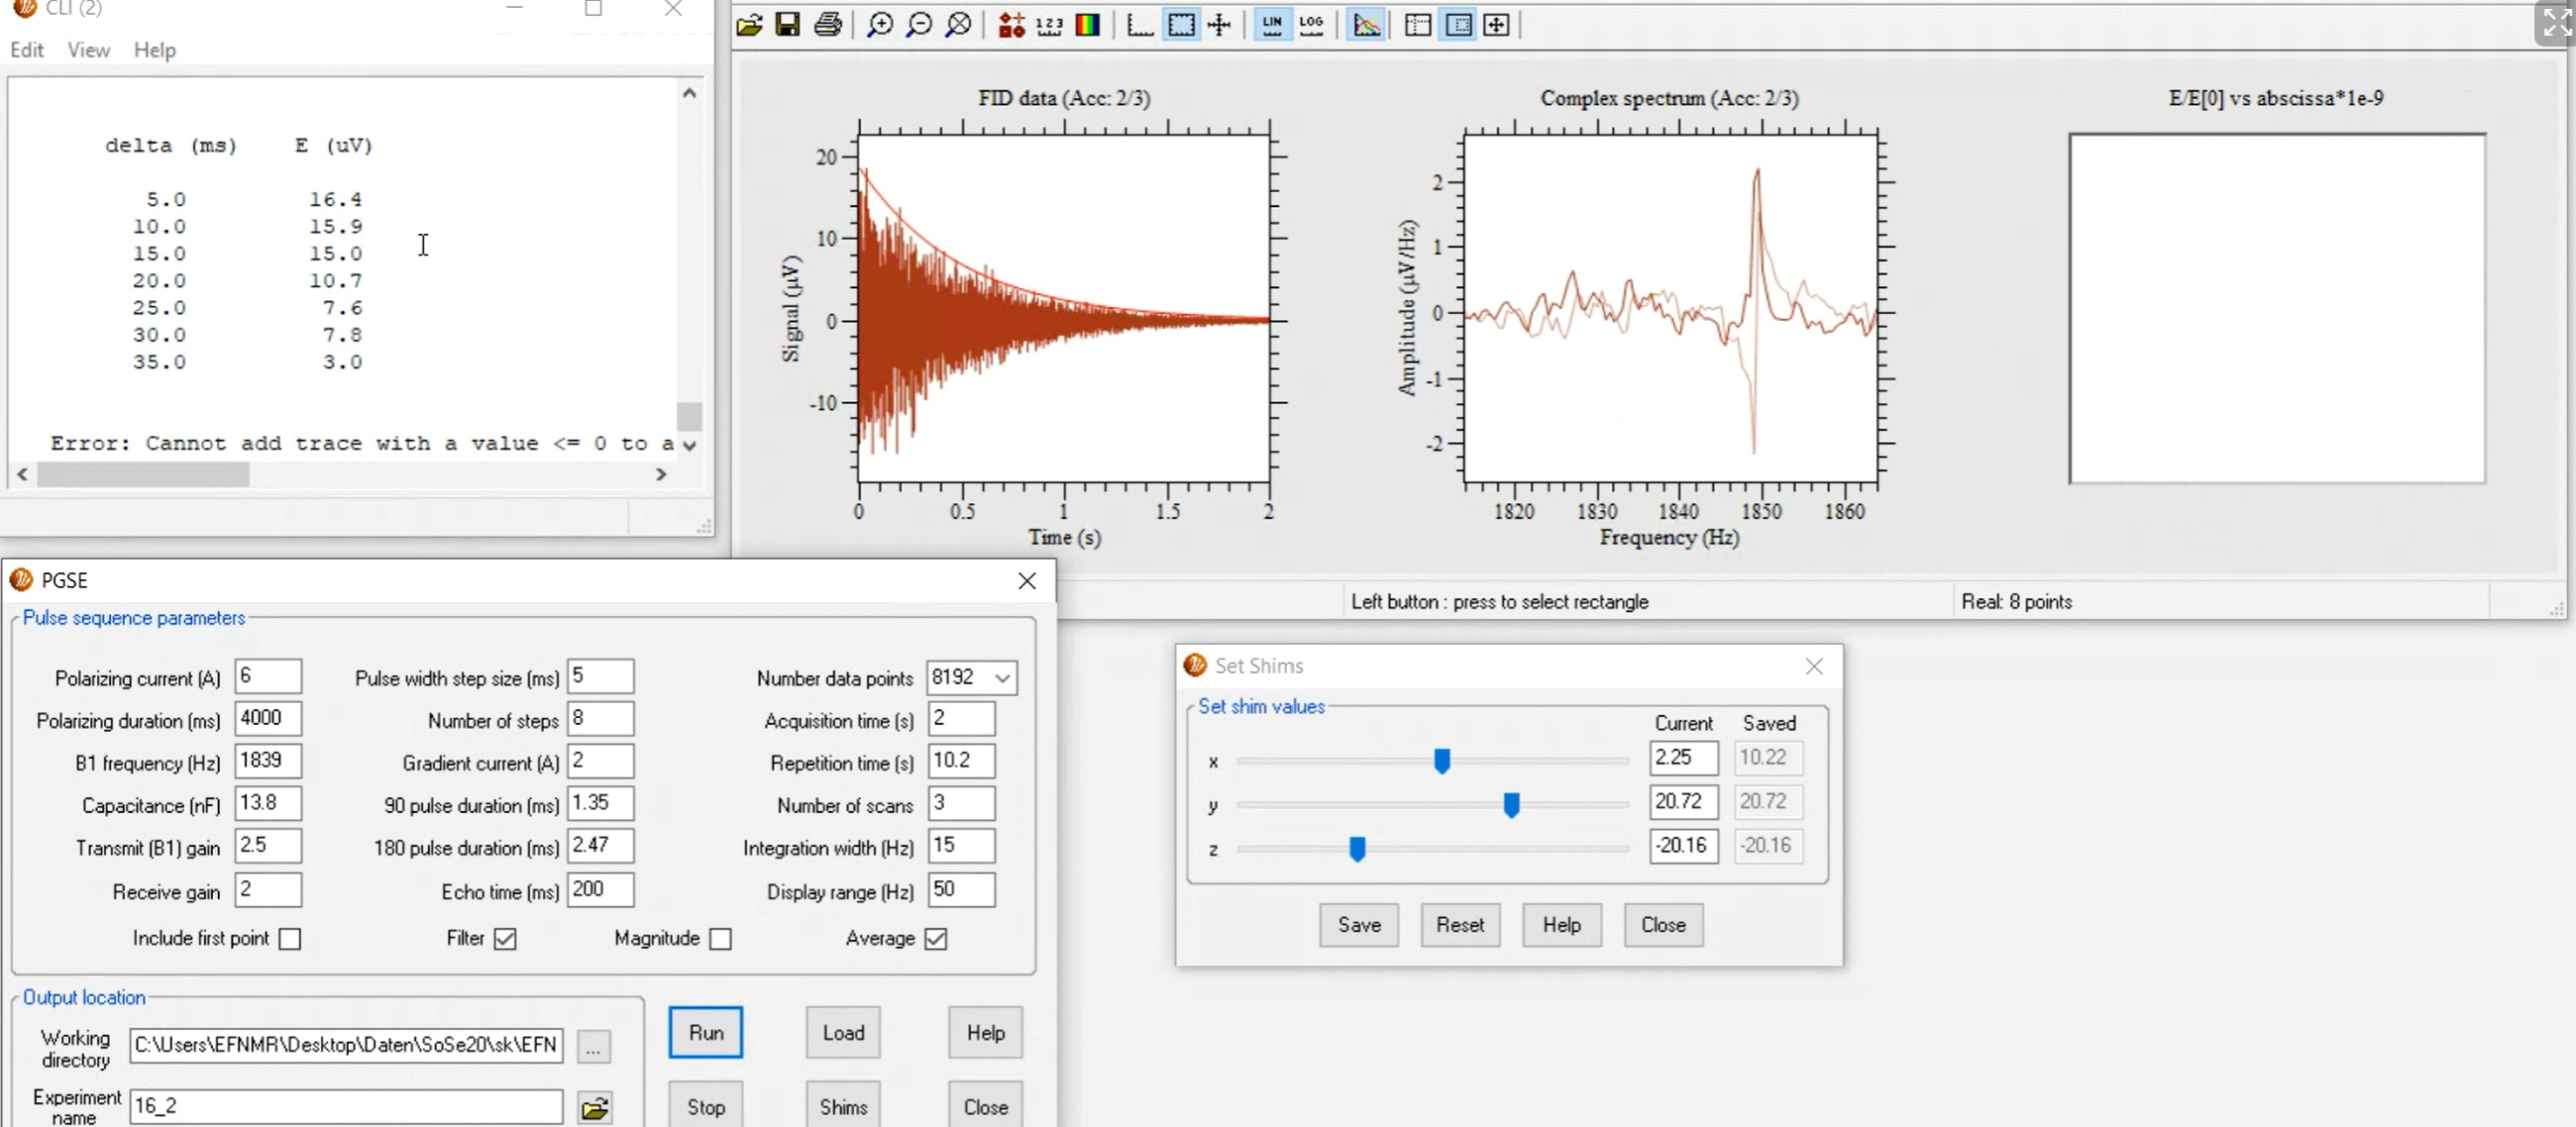
\includegraphics[width = 0.9 \textwidth]{Screenshot2/16_2.jpg}
    \caption{Konzentrationen der Verfügbaren Proben}
\end{figure}


\begin{figure}[H]
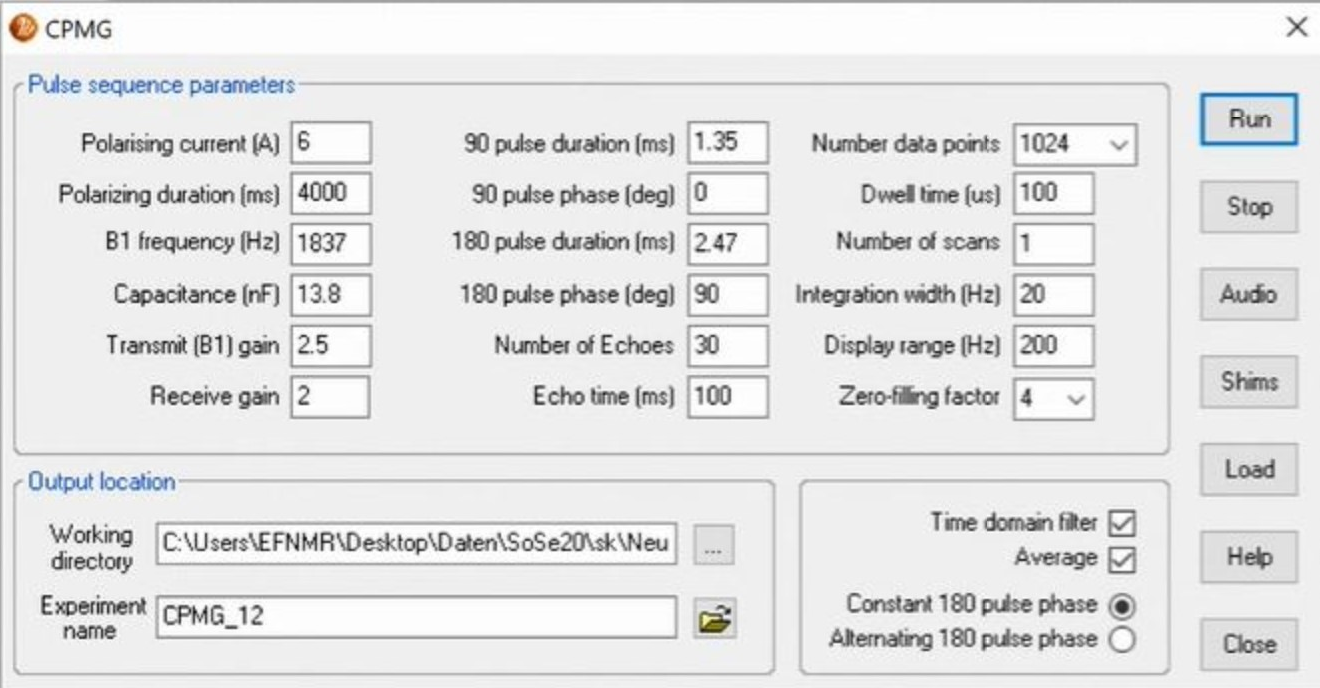
\includegraphics[width = \textwidth]{1.png}
\caption{1}
\label{1}
\end{figure}

\begin{figure}[H]
    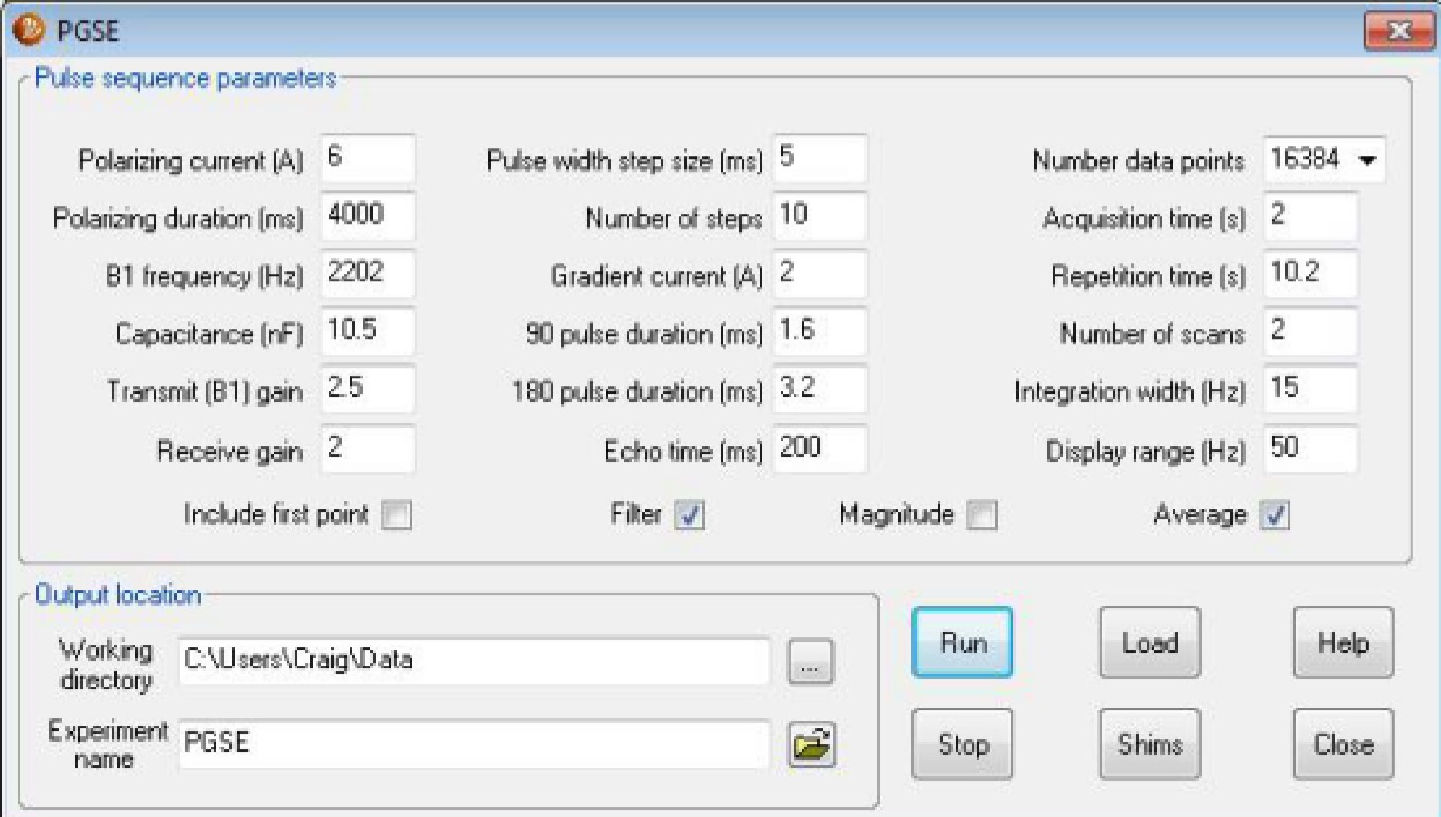
\includegraphics[width = \textwidth]{2.png}
    \caption{2}
    \label{2}
    \end{figure}
    % \begin{enumerate}

    %     \item Einloggen und einrichten des Dateipfades (18:20)
    %     \item EFNMR Werte von dem ersten Versuchstag wiederholen oder als gelich angenommen werden(Teil 6.4.1 im Usermanual)(Am ersten Versuchstag ca. 3 Stunden eingeplant)
    %     \item $T_1$ und $T_2$ werden jeweils in Abhängigkeit von der Konzentration der Lösung bestimmt(Welche Auswirkung das $CUSO_4$ (paramagnetisches Salz?) auf das $H^1$ Spektrum vom Wasser hat; Proben enthalten  Konzentratrionen zwischen $\SI{250}{$\mu$ \textsc{M}}$ bis $\SI{5000}{$\mu$ \textsc{M}}$ $\Longrightarrow$ Auftragen der Relaxationszeiten über die Konzentration um Relaxitivität $r_1$ bzw. $r_2$ erhalten; (2 Stunden)
    %     \item 1-D Bild erstellen mit Gradient echo imaging;(30 min)
    %     \item Untersuchung der Kopplungskonstante (J-Kopplung) von 2,2,2 Flurethanol; Signalaufnahme mit veränderten anregungsfrequenzen und veränderter Resonanzbedingung im Schwingkreis (1 Stunde)
    %     \item 2-D nD Gradient-Echo; veränderung des Gradientens entlang der x,y-Achse und zusätzlich die Gewichtung der Relaxationszeit, sodass man die Röhren einzelnd sehen kann (30 min)
    %     \item PGSE-Experiment; nach dem $90^{\degree}$ und $180^{\degree}$ Puls werden jeweils kurze Gradientenfelder angelegt um auf die Selbstdiffusion im Wasser zu untersuchen (30 min)
    %     \end{enumerate}
\end{document}